%!TEX encoding = UTF-8 Unicode
\documentclass[a4paper]{compendium}
\usepackage[swedish]{babel}

%\usepackage{xr} %to crossreference ???
\externaldocument{compendium} %to crossreference to compendium.tex

\addto\captionsswedish{%
  \renewcommand{\appendixname}{Appendix}%
}
%TODO: Glossary
%http://tex.stackexchange.com/questions/5821/creating-a-standalone-glossary/5837#5837

\setlength{\columnsep}{16mm}

\newcommand{\LibVersion}{1.3.1} % latest version of introlib at https://github.com/lunduniversity/introprog-scalalib
\newcommand{\LibJar}{\texttt{introprog\_3-\LibVersion.jar}}
\newcommand{\JDKApiUrl}{\url{https://docs.oracle.com/en/java/javase/17/docs/api/}}
\newcommand{\CurrentYear}{2024}
\newcommand{\VMName}{vm2020} %TODO: update vm
\newcommand{\VMPassword}{pgkBytMig2020}
\newcommand{\VirtualBoxVersion}{7.0} %https://www.virtualbox.org/wiki/Downloads
\newcommand{\UbuntuVersion}{22.04}
\newcommand{\ScalaVersion}{3.4.2} %https://www.scala-lang.org/
\newcommand{\SbtVersion}{1.10.0} %https://eed3si9n.com/category/tags/sbt
\newcommand{\JDKVersion}{17} %https://adoptium.net/temurin/releases/?version=17
\newcommand{\KojoVersion}{2.9.28} %https://www.kogics.net/kojo-download
\newcommand{\VSCodeVersion}{1.90} %https://code.visualstudio.com/updates
\newcommand{\MetalsVersion}{v1.35} %https://marketplace.visualstudio.com/items?itemName=scalameta.metals
\newcommand{\WindowsVersion}{10}
\newcommand{\ScalaIDEVersion}{4.7.0} %%DEPRECATED
\newcommand{\OmkontrollDatum}{Torsd. 14/11 kl 13:00-18:00, E:1147}%Tors W09; används i lect-w08 och lect-w09
\newcommand{\LastLectureDate}{onsdagen den 6:e december i E:A kl 10-12}





\title{
{\vspace{-3.0cm}\bf\sffamily\Huge\selectfont  Introduktion till programmering med Scala}
\\ \vspace{1em}%\hspace*{1.5cm}\inputgraphics[width=0.6\textwidth]{../img/gurka} \\
{\sffamily  Föreläsningar}\\\vspace{2cm}
%\includegraphics[height=4cm]{../img/scala-logo.png}
%\includegraphics[height=4cm]{../img/java-logo.png}
\includegraphics[height=12cm]{cover/gurka.jpg}
}

%\author{Redaktör: Björn Regnell}
\date{\raggedbottom%
\vspace{-2em}\begin{minipage}{1.0\textwidth}\centering
\CourseCode, Lp1-2, HT \CurrentYear\\
Datavetenskap, LTH\\
Lunds Universitet\\
~\\
Kompileringsdatum: \today \\
\url{https://lunduniversity.github.io/pgk}
\end{minipage}
}

\usepackage{multicol}

\usepackage{tikz}
\usetikzlibrary{shapes.geometric, shapes.symbols, arrows, matrix, shapes, positioning, calc}
\usepackage{tkz-euclide}
%\usetkzobj{all} %%% AAAARGH Version clash, broken api :(
  % Work-around: dont't use \tkzLabel \tkzMarkAngle, 
  %  prev. used in w05-classes and lect-w05 but now replaced by a hack 
%https://tex.stackexchange.com/questions/529550/latex-cant-find-file-tkz-obj-angles-tex


\usepackage{pgffor}  %% http://stackoverflow.com/questions/2561791/iteration-in-latex
                     %  allows:  \foreach \n in {1,...,4}{ do something with \n }

\usepackage{framed}  %  allows:   \begin{framed}\end{framed}
%\newenvironment{Slide}[2][]
%  {\begin{framed}\setlist{noitemsep}\section*{#2}}
%  {\end{framed}}


\newcommand{\SlideHeading}[1]{\section*{#1}}

\usepackage[most]{tcolorbox}
\newenvironment{Slide}[2][]
  {\vspace{0.5em}\begin{tcolorbox}[left=1.5em,%width=1.05\textwidth,
  grow to right by=0.05\textwidth,grow to left by=0.05\textwidth,%
  %breakable,
  %frame hidden,
  colframe=gray!20,
  enhanced]\setlist{noitemsep}\SlideHeading{#2}}
  {\end{tcolorbox}\vspace{0.5em}}

\newcommand{\Subsection}[1]{} %ignore slide sections
\newcommand{\SlideOnly}[1]{} %ignore slide font size

\usepackage[framemethod=tikz]{mdframed}

\newif\ifkompendium  % to allow conditional text in slides only showing up in compendium
\kompendiumtrue      % in slides: \kompendiumfalse

\newif\ifPreSolution  % to allow tasks and solutions in same file
\PreSolutiontrue      % in solutions: \PreSolutionfalse

%!TEX encoding = UTF-8 Unicode

\newcommand{\ModWeekONE}{Introduktion}
\newcommand{\ExeWeekONE}{expressions}
\newcommand{\LabWeekONE}{kojo}


\newcommand{\ModWeekTWO}{Program och kontrollstrukturer}
\newcommand{\ExeWeekTWO}{programs}
\newcommand{\LabWeekTWO}{--}


\newcommand{\ModWeekTHREE}{Funktioner och abstraktion}
\newcommand{\ExeWeekTHREE}{functions}
\newcommand{\LabWeekTHREE}{irritext}


\newcommand{\ModWeekFOUR}{Objekt och inkapsling}
\newcommand{\ExeWeekFOUR}{objects}
\newcommand{\LabWeekFOUR}{blockmole}


\newcommand{\ModWeekFIVE}{Klasser och datamodellering}
\newcommand{\ExeWeekFIVE}{classes}
\newcommand{\LabWeekFIVE}{blockbattle0}


\newcommand{\ModWeekSIX}{Mönster och felhantering}
\newcommand{\ExeWeekSIX}{patterns}
\newcommand{\LabWeekSIX}{blockbattle1}


\newcommand{\ModWeekSEVEN}{Sekvenser och enumerationer}
\newcommand{\ExeWeekSEVEN}{sequences}
\newcommand{\LabWeekSEVEN}{shuffle}


\newcommand{\ModWeekEIGHT}{Nästlade och generiska strukturer}
\newcommand{\ExeWeekEIGHT}{matrices}
\newcommand{\LabWeekEIGHT}{life}


\newcommand{\ModWeekNINE}{Mängder och tabeller}
\newcommand{\ExeWeekNINE}{lookup}
\newcommand{\LabWeekNINE}{words}


\newcommand{\ModWeekTEN}{Arv och komposition}
\newcommand{\ExeWeekTEN}{inheritance}
\newcommand{\LabWeekTEN}{snake0}


\newcommand{\ModWeekELEVEN}{Varians och kontextparametrar}
\newcommand{\ExeWeekELEVEN}{context}
\newcommand{\LabWeekELEVEN}{snake1}


\newcommand{\ModWeekTWELVE}{Valfri fördjupning, Projekt}
\newcommand{\ExeWeekTWELVE}{extra}
\newcommand{\LabWeekTWELVE}{Projekt0}


\newcommand{\ModWeekTHIRTEEN}{Repetition}
\newcommand{\ExeWeekTHIRTEEN}{examprep}
\newcommand{\LabWeekTHIRTEEN}{Projekt1}


\newcommand{\ModWeekFOURTEEN}{MUNTLIGT PROV}
\newcommand{\ExeWeekFOURTEEN}{Munta}
\newcommand{\LabWeekFOURTEEN}{Munta}


\begin{document}

\pagenumbering{roman}

\frontmatter
\maketitle
%!TEX encoding = UTF-8 Unicode
%!TEX root = ../compendium.tex

\clearpage\null\thispagestyle{empty}
\vfill

{
\setlength{\parindent}{0pt}
\emph{Editor}: Björn Regnell \\

%  LIST OF CONTRIBUTORS to https://github.com/lunduniversity/introprog
%    Please contact bjorn.regnell@cs.lth.se if you think you should be
%    on this list, or make a pull request with an update of file briefly
%    describing your contribution in the commit text.
%    This work is licenced under CC-BY-SA-4.0.
%!TEX encoding = UTF-8 Unicode
%!TEX root = compendium/compendium.tex
\hyphenation{Borg-lund Da-ne-bjer Grampp Palm-qvist Ravn-borg Ro-sen-qvist Schrei-ter Wih-lan-der}
\emph{Contributors} in alphabetical order:
Anders Buhl,
André Philipsson Eriksson,
Anna Axelsson,
Anna Palmqvist Sjövall,
Annie Predel,
Anton Andersson,
Benjamin Lindberg,
Björn Regnell,
Casper Schreiter,
Cecilia Lindskog,
Dag Hemberg,
Elias Åradsson,
Elliot Bräck,
Elsa Cervetti Ogestad,
Emelie Engström,
Emil Wihlander,
Erik Bjäreholt,
Erik Grampp,
Evelyn Beck,
Felix Ohrgren,
Fredrik Danebjer,
Fritjof Bengtsson,
Gustav Cedersjö,
Henrik Olsson,
Hjalmar Rutberg,
Hussein Taher,
Jakob Hök,
Jakob Sinclair,
Johan Ravnborg,
Jonas Danebjer,
Jos Rosenqvist,
Maj Stenmark,
Maria Kulesh,
Måns Magnusson,
Nicholas Boyd Isacsson,
Niklas Sandén,
Oliver Levay,
Oliver Persson,
Oscar Sigurdsson,
Oskar Berg,
Oskar Widmark,
Patrik Persson,
Per Holm,
Philip Sadrian,
Sandra Nilsson,
Sebastian Hegardt,
Simon Persson,
Stefan Jonsson,
Theodor Lundqvist,
Tim Borglund,
Tom Postema,
Valthor Halldorsson,
Viktor Claesson,
Wilhelm Wanecek,
William Karlsson.
\\ \newline

\emph{Home}: \url{https://cs.lth.se/pgk} \newline

\emph{Repo}: \url{https://github.com/lunduniversity/introprog} \\ \newline

This compendium is on-going work. \\ \textbf{Contributions are welcome!} \\
\emph{Contact}: \url{bjorn.regnell@cs.lth.se}
\\ \newline

%\emph{Cover art}: Björn Regnell (inspired by Poul Ströyer's illustration of Lennart Hellsing's lyrics to  the childrens song ''Herr Gurka'' with music by Knut Brodin)\\ \newline

\emph{Versions:} \\
Scala \ScalaVersion \\
JDK \JDKVersion\\
\href{https://github.com/lunduniversity/introprog-scalalib/}{introprog-scalalib} \LibVersion \\ 

\vfill

You can use this work if you respect this \textbf{LICENSE}: CC BY-SA 4.0 \\
\url{http://creativecommons.org/licenses/by-sa/4.0/} \\
\textbf{Do \emph{not} distribute solutions to lab assignments and projects.}
\\ \newline
Copyright \copyright~ 2015-\CurrentYear. \\
Björn Regnell, Dept. of Computer Science, LTH, Lund University.\\
}

%!TEX encoding = UTF-8 Unicode
%!TEX root = ../compendium.tex

\ChapterUnnum{Framstegsprotokoll}\label{progress-protocoll}


\section*{Genomförda övningar}

\vspace{1em}\noindent
{Till varje laboration hör en övning med uppgifter som utgör förberedelse inför labben. Du behöver minst behärska grunduppgifterna för att klara labben inom rimlig tid. Om du känner att du behöver öva mer på grunderna, gör då även extrauppgifterna. Om du vill fördjupa dig, gör fördjupningsuppgifterna som är på mer avancerad nivå. Kryssa för nedan vilka övningar du har gjort, så blir det lättare för din handledare att anpassa dialogen till de kunskaper du förvärvat hittills.}

%% COMPATIBILITY PROBLEM In latex --version 2022 \bottomrule \addlinespace \midrule \toprule etc gives error ! Misplaced \noalign.
%% Here they are replaced by \hline and \\[1.2em]  etc
%% The commands from the booktab chapter are thus cancelled here; can the booktab package be removed?

\newcommand{\TickBox}{\raisebox{-.50ex}{\Large$\square$}}
\newcommand{\ExeRow}[1]{\hyperref[section:exe:#1]{\texttt{#1}} & \TickBox  &  \TickBox &  \TickBox  \\ } %\addlinespace }

\begin{table}[h]
%\centering
\vspace{2em}
\begin{tabular}{lccc}
\hline \\ %\toprule 
%\addlinespace
{\sffamily Övning} &
{\sffamily Grund} &
{\sffamily Extra} &
{\sffamily Fördjupning} \\[1em] \hline  %\addlinespace \midrule \\[-0.7em]  
\\

\input{../compendium/generated/exercises-generated.tex}
\\\hline%\bottomrule 
\end{tabular}
\end{table}

\newpage

\section*{Godkända obligatoriska moment}

\vspace{1em}\noindent
För att bli godkänd på laborationsuppgifterna och projektuppgiften måste du lösa deluppgifterna och diskutera dina lösningar med en handledare. Denna diskussion är din möjlighet att få feedback på dina lösningar. Ta vara på den!
Se till att handledaren noterar nedan när du har blivit godkänd på respektive obligatoriska moment. Spara detta blad tills du fått slutbetyg i kursen.


\vspace{2.2em}\noindent Namn: \dotfill\\

\vspace{1em}\noindent Namnteckning: \dotfill\\

\newcommand{\LabRow}[1]{\\[-1.1em] \hyperref[section:lab:#1]{\texttt{#1}} & \dotfill &  \dotfill  \\[0.7em]}  %\addlinespace }

\begin{table}[h]
%\centering
\vspace{1em}
\begin{tabular}{lcc}
\hline%\toprule\addlinespace
\\
{\sffamily\bfseries\small Lab} & {\sffamily\small kompl+datum,gk+datum } &	
{\sffamily\small Handl. underskr. + namnförtydl.}\\ %\addlinespace 
%\midrule 
\\[-0.5em]
%!TEX encoding = UTF-8 Unicode
%!TEX root = ../compendium.tex
\LabRow{kojo}
\LabRow{irritext}
\LabRow{blockmole}
\LabRow{blockbattle0}
\LabRow{blockbattle1}
\LabRow{shuffle}
\LabRow{life}
\LabRow{words}
\LabRow{snake0}
\LabRow{snake1}
%\toprule
%\addlinespace
\\ 
%\midrule 
%\addlinespace\addlinespace
{\sffamily\small {\bfseries Projektuppgift}} & \dotfill &  \dotfill  \\
%\addlinespace\addlinespace %\midrule
\\
{\Large$\square$}\texttt{~~~\hyperref[section:proj:bank]{bank}} &
\multicolumn{2}{c}{\textit{Om egendef., ge kort beskrivning här:}}  \\[0.6em] %\addlinespace
%{\Large$\square$}\texttt{~~~\hyperref[section:proj:tabular]{tabular}} \\[0.6em] %\addlinespace
{\Large$\square$}\texttt{~~~\hyperref[section:proj:music]{music}} \\[0.6em] %\addlinespace
{\Large$\square$}\texttt{~~~\hyperref[section:proj:photo]{photo}}  \\[0.6em] %\addlinespace
{\Large$\square$}\texttt{~~~}\textit{egendefinerad}  \\
%\dotfill  \\
%\addlinespace\addlinespace
\\
%\midrule
% \addlinespace
\\
{\sffamily\small {\bfseries Muntligt prov}} &  & \\
%\addlinespace\addlinespace{}
\\
{\Large$\square$}\texttt{~~~} godkänd & \dotfill &  \dotfill \\
%\addlinespace\addlinespace
\\\hline%\bottomrule
\end{tabular}
\end{table}

\input{prechapters/preface.tex}

\setcounter{tocdepth}{2} % set headings level in table of contents
\tableofcontents
\mainmatter

\pagenumbering{arabic}

\part{Om kursen}
\setcounter{chapter}{-3}
\input{prechapters/course-architecture.tex}
%!TEX encoding = UTF-8 Unicode
%!TEX root = ../compendium.tex

\hyphenation{för-kun-skaps-en-kät}
\hyphenation{grupp-lä-ran-de}

\chapter{Anvisningar}

Detta kapitel innehåller anvisningar och riktlinjer för kursens olika delar. Läs noga så att du inte missar viktig information om syftet bakom kursmomenten och vad som förväntas av dig.

\section{Samarbetsgrupper}

Ditt lärande i allmänhet, och ditt programmeringslärande i synnerhet, fördjupas om det sker i dialog med andra. Dessutom är din samarbetsförmåga och din pedagogiska förmåga avgörande för din framgång som professionell systemutvecklare. Därför är kursdeltagarna indelade i \emph{samarbetsgrupper} om 4-6 personer där medlemmarna samverkar för att alla i gruppen ska nå så långt som möjligt i sina studier.

För att hantera och dra nytta av skillnader i förkunskaper är samarbetsgrupperna indelade så att deltagarna har \emph{varierande förkunskaper} baserat på en förkunskapsenkät. De som redan har provat på att programmera får då chansen att träna på sin pedagogiska förmåga som är så viktig för systemutvecklare, medan de som ännu inte kommit lika långt kan dra nytta av gruppmedlemmarnas samlade kompetens i sitt lärande. Kompetensvariationen i gruppen kommer att förändras under kursens gång, då olika individer lär sig olika snabbt i olika skeden av sitt lärande; de som till att börja med har ett försprång kanske senare får kämpa för att komma över en viss lärandetröskel.

Samarbetsgrupperna organiserar själva sitt arbete och varje grupp får finna de samarbetsformer som passar medlemmarna bäst. Här följer några erfarenhetsbaserade tips:

\begin{enumerate}
\item Träffas så fort som möjligt i hela gruppen och lär känna varandra. Ju snabbare ni kommer samman som grupp och får den sociala interaktionen att fungera desto bättre. Ni kommer att ha nytta av denna investering under hela terminen och kanske under resten av er studietid.
\item Kom överens om stående mötestider och mötesplatser. Det är viktigt med kontinuiteten i arbetet för att samarbetet i gruppen ska utvecklas och fördjupas. Träffas minst en gång i veckan. Ha en stående agenda, t.ex. en runda runt bordet där var och en berättar hur långt hen kommit och listar de begreppen som hen för tillfället behöver fokusera på.
\item Hjälps åt att tillsammans identifiera och diskutera era olika individuella studiebehov och studieambitioner. När man ska lära sig att programmera stöter man på olika lärandetrösklar som man kan få hjälp att ta sig över av någon som redan är förbi tröskeln. Men det gäller då för den som hjälper att först förstå exakt vad det är som är svårt, eller vilka specifika pusselbitar som saknas, för att på bästa sätt kunna underlätta för en medstudent att ta sig över tröskeln. Det gäller att hjälpa \emph{lagom} mycket så att var och en självständigt får chansen att skriva sin egen kod.
\item Var en schysst kamrat och agera professionellt, speciellt i situationer där gruppdeltagarna vill olika. Kommunicera på ett respektfullt sätt och sök konstruktiva kompromisser. Att utvecklas socialt är viktigt för din framtida yrkesutövning som systemutvecklare och i samarbetsgruppen kan du träna och utveckla din samarbetsförmåga.
\end{enumerate}

\subsection{Samarbetskontrakt}

Ni ska upprätta ett samarbetskontrakt redan under första veckan och visa för en handledare. Alla gruppmedlemmarna ska skriva under kontraktet. Handledaren ska också skriva under som bekräftelse på att ni visat kontraktet.

Syftet med kontraktet är att ni ska diskutera igenom i gruppen hur ni vill arbeta och vilka regler ni tycker är rimliga. Ni bestämmer själva vad kontraktet ska innehålla. Nedan finns förslag på punkter som kan ingå i ert kontrakt. En kontraktsmall finns här: \url{https://github.com/lunduniversity/introprog/blob/master/study-groups/collaboration-contract.tex}

\begin{oframed}
\noindent\textbf{Samarbetskontrakt}\\
Vi som skrivit under detta kontrakt lovar att göra vårt bästa för att följa samarbetsreglerna nedan, så att alla ska lära sig så mycket som möjligt.
\begin{enumerate}
\item Komma i tid till gruppmöten.
\item Vara väl förberedda genom självstudier inför gruppmöten.
\item Hjälpa varandra att förstå, men inte lösa uppgifter åt någon annan.
\item Ha ett respektfullt bemötande även om vi har olika åsikter.
\item Inkludera alla i gemenskapen.
\item ...
\end{enumerate}
\end{oframed}
\subsection{Grupplaboration}\label{subsection:grouplabs}
Laboration \texttt{\LabWeekTEN} i läsvecka W10 är en grupplaboration.
Följande anvisningar gäller speciellt för grupplaborationen. (Allmänna anvisningar som gäller för både de individuella laborationerna och grupplaborationer finns i avsnitt \ref{section:labs}.)

\begin{enumerate}
\input{team-lab-prep-items.tex}
\end{enumerate}

\subsection{Samarbetsbonus}\label{section:bonus}

Alla tjänar på att samarbeta och hjälpa varandra i lärandet. Som extra incitament för grupplärande utdelas \emph{samarbetsbonus} baserat på resultatet från den diagnostiska kontrollskrivningen efter halva kursen (se avsnitt \ref{section:diagnostic-test}). Bonus ges till varje student enligt gruppmedelvärdet av kontrollskrivningspoängen och räknas ut med funktionen \code{collaborationBonus} nedan, där \code{points} är en sekvens med heltal som utgör gruppmedlemmars individuella poäng från kontrollskrivningen.

\begin{Code}
  def collaborationBonus(points: Seq[Int]): Int =
    (points.sum / points.size.toDouble).round.toInt
\end{Code}

Samarbetsbonusen viktas så att den högsta möjliga bonusen maximalt utgör $5\%$ av maxpoängen på tentan och adderas till det individuella tentaresultatet om du är godkänd på kursens sluttentamen. Samarbetsbonusen kan alltså påverka om du når högre betyg, men den påverkar \emph{inte} om du får godkänt eller ej. Detta gör att alla i gruppen gynnas av att så många som möjligt lär sig på djupet inför kontrollskrivningen. Din eventuella samarbetsbonus räknas dig tillgodo endast vid det första, ordinarie tentamenstillfället.

\section{Föreläsningar}

En normal läsperiodsvecka börjar med två föreläsningspass om $2$ timmar vardera. Föreläsningarna ger en översikt av kursens teoretiska innehåll och går igenom innebörden av de begrepp du ska lära dig. Föreläsningarna innehåller många programmeringsexempel och föreläsaren ''lajvkodar'' då och då för att illustrera den kreativa problemlösningsprocess som ingår i all programmering. Föreläsningarna berör även kursens organisation och olika praktiska detaljer.

På föreläsningarna ges goda möjligheter att ställa allmänna frågor om teorin och att i plenum diskutera specifika svårigheter (individuell lärarhjälp ges på resurstider, se avsnitt \ref{section:tutorials}, och på laborationer, se avsnitt \ref{section:labs}). Även om det är många i föreläsningssalen, \emph{tveka inte att ställa frågor} -- det är säkert fler som undrar samma sak som du!

Föreläsningarna är inte obligatoriska, men det är mycket viktigt att du går dit, även om du i perioder känner att du har bra koll på all teori. På föreläsningarna får du en övergripande ämnesstruktur och en konkret programmeringsupplevelse, som du delar med dina kursare och kan diskutera i samarbetsgrupperna. Föreläsningarna ger också en prioritering av materialet och förbereder dig inför examinationen med praktiska råd och tips om hur du bör fokusera dina studier.

\section{Övningar}

I en normal läsperiodsvecka ingår en övning med flera uppgifter och deluppgifter.
Övningarna utgör grunden för dina programmeringsstudier och erbjuder en systematisk genomgång av kursteorins alla delar genom praktiska kodexempel som du genomför steg för steg vid datorn med hjälp av ett interaktivt verktyg som kallas Read-Evaluate-Print-Loop (REPL). Om du gör övningarna i REPL säkerställer du att du skaffar dig tillräcklig förståelse för alla begrepp som ingår i kursen och att du inte missar någon viktig pusselbit.

Övningarna fungerar också som förberedelse inför laborationerna. Om du inte gör veckans övning är det inte troligt att du kommer att klara veckans laboration inom rimlig tid.

Två saker är särskilt viktiga när du lär dig att programmera:
\begin{itemize}
\item \textbf{Programmera!} Det räcker inte med att bara passivt läsa om programmering; du måste \emph{aktivt} själv skriva mycket kod och genomföra egna programmeringsexperiment. Det underlättar stort om du bejakar din nyfikenhet och experimentlusta. Alla programmeringsfel som du gör och alla dina misstag, som i efterhand verkar enkla, är i själva verket oumbärliga steg på vägen och ger avgörande \emph{''Aha!''}-upplevelser. Kursens övningar är grunden för denna form av lärande.

\item \textbf{Ha tålamod!} Det är först när du har förmågan att aktivt kombinera \emph{många} olika programmeringskoncept som du själv kan lösa lite större programmeringsuppgifter. Det kan vara frustrerande i början innan du når så långt att din verktygslåda med begrepp är tillräckligt stor för att du ska kunna skapa den kod du vill. Ibland krävs det extra tålamod innan allt plötsligt lossnar. Många programmeringslärare och -studenter vittnar om att ''polletten plötsligt trillar ner'' och allt faller på plats. Övningarna syftar till att, steg för steg, bygga din verktygslåda så att den till slut blir tillräckligt kraftfull för mer avancerad problemlösning.
\end{itemize}

Olika studenter har olika ambitionsnivå, skilda förkunskaper, varierande arbetskapacitet, mer eller mindre välutvecklad studieteknik och olika lätt för att lära sig att programmera. För att hantera denna variation erbjuds övningsuppgifter av tre olika typer:

\begin{itemize}
\item \textbf{Grunduppgifter}. Varje veckas grunduppgifter täcker basteorin och hjälper dig att säkerställa att du kan gå vidare utan kunskapsluckor. Grunduppgifterna utgör även basen för laborationerna. Alla studenter bör göra alla grunduppgifter. En bra förståelse för innehållet i grunduppgifterna ger goda förutsättningar att klara godkänt betyg på sluttentamen.

\item \textbf{Extrauppgifter}. Om du upplever att grunduppgifterna är svåra och du vill öva mer, eller om du vill vara säker på att du verkligen befäster dina grundkunskaper, då ska du göra extrauppgifterna. Dessa är på samma nivå som grunduppgifterna och ger extra träning.

\item \textbf{Fördjupningsuppgifter}. Om du vill gå djupare och har kapacitet att lära dig ännu mer, gör då fördjupningsuppgifterna. Dessa kompletterar grunduppgifterna med mer avancerade exempel och går utöver vad som krävs för godkänt på kursen. Om du satsar på något av de högre betygen ska du göra fördjupningsuppgifterna.
\Uberkurs Vissa fördjupningsuppgifter har en stjärna i marginalen. Denna symbol visar att uppgiften är allmänbildande, men överkurs och kommer ej på tentamen.

\end{itemize}


Till varje övning finns lösningar som du hittar längst bak i detta kompendium. Titta \emph{inte} på lösningen innan du själv först försökt lösa uppgiften. Ofta innehåller lösningarna kommentarer och tips så glöm inte att kolla igenom veckans lösningar innan du börjar förbereda dig inför veckans  laboration.

Tänk på att det ofta finns \emph{många olika lösningar} på samma programmeringsproblem, som kan vara likvärdiga eller ha olika fördelar och nackdelar beroende på sammanhanget. Diskutera gärna olika lösningsvarianter med dina kursare och handledare -- att prova många olika sätt att lösa en uppgift fördjupar ditt lärande avsevärt!

Många uppgifter lyder ''testa detta i REPL och förklara vad som händer'' och svårigheten ligger ofta inte i att skapa själva koden utan att förstå hur den fungerar och \emph{varför}. På detta sätt tränar du ditt programmeringstänkande med hjälp av en växande begreppsapparat. Syftet är ofta att illustrera ett allmängiltigt koncept och det är därför extra bra om du skapar egna övningsuppgifter på samma tema och experimenterar med nya varianter som ger dig ytterligare förståelse.

Övningsuppgifterna innehåller ofta färdiga kodsnuttar som du ska skriva in i REPL medan den kör i ett terminalfönster. REPL-kod visas i övningsuppgifterna med ljus text på mörk bakgrund, så här:
%\begin{mdframed}[backgroundcolor=black!80,leftmargin=0.1cm,rightmargin=0.1cm,skipabove=0.2cm,hidealllines=true,  innerleftmargin=0.1cm,innerrightmargin=0.1cm,innertopmargin=-0.3cm,innerbottommargin=-0.3cm]
\begin{REPL}
scala> val msg = "Hello world!"
scala> println(msg)
\end{REPL}
%\end{mdframed}
Prompten \code{scala>} indikerar att REPL är igång och väntar på indata. Du ska skriva den kod som står \emph{efter} prompten. Mer information om hur du använder REPL hittar du i appendix \ref{appendix:compile:REPL}.

Även om kompendiet finns tillgängligt för nedladdning, frestas \emph{inte} att klippa ut och klistra in alla kodsnuttar i REPL. Ta dig istället den ringa tiden det tar att skriva in koden rad för rad. Medan du själv skriver hinner du tänka efter, och det egna, aktiva skrivandet främjar ditt lärande och gör det lättare att komma ihåg och förstå.


\section{Resurstider}\label{section:tutorials}

Under varje läsperiodsvecka finns ett flertal resurstider i schemat. Det finns minst en tid som passar din schemagrupp, men du får gärna gå på andra och/eller flera tider i mån av plats. Resurstiderna är schemalagda i datorsal med Linuxdatorer och i varje sal finns en handledare som är redo att svara på dina frågor.

Följande riktlinjer gäller för resurstiderna:

\begin{enumerate}
\item \textbf{Syfte}. Resurstiderna är primärt till för att hjälpa dig vidare om du kör fast med övningarna eller laborationsförberedelserna, men du får fråga om vad som helst som rör kursen i den mån handledaren kan svara och hinner med.

\item \textbf{Samarbete}. Hjälp gärna varandra under resurstiderna! Om någon kursare kör fast är det utvecklande och lärorikt att hjälpa till. Om schema och plats tillåter kan du gärna gå på samma resurstidstillfälle som någon medlem i din samarbetsgrupp, men ni kan också lika gärna hjälpas åt tvärs över gruppgränserna.

\item \textbf{Hänsyn}. När du hjälper andra, tänk på att prata riktigt tyst så att du inte stör andras koncentration. Tänk också på att alla behöver träna mycket själv utan att bli alltför styrda av en ''baksätesförare''. Ta inte över tangentbordet från någon annan; ge hellre välgenomtänkta tips på vägen och låt din kursare behålla kontrollen över uppgiftslösningen.


\item \textbf{Fokus}. Du ska \emph{inte} göra och redovisa laborationen på resurstiderna; dessa ska göras och redovisas på laborationstid. Men om du varit sjuk eller ej blivit godkänd på någon enstaka laboration kan du, om handledaren så hinner, be att få redovisa din restlaboration på en resurstid.

\item \textbf{Framstegsprotokoll}. På sidan \pageref{progress-protocoll} finns ett framstegsprotokoll för övningarna. Håll detta uppdaterat allteftersom du genomför övningarna och visa protokollet när du frågar om hjälp av handledare. Då blir det lättare för handledaren att se vilka kunskaper du förvärvat hittills och anpassa dialogen därefter.


\end{enumerate}
\section{Laborationer}\label{section:labs}

En normal läsperiodsvecka avslutas med en lärarhandledd laboration. Medan övningar tränar teorins olika delar i många mindre uppgifter, syftar laborationerna till träning i att kombinera flera begrepp och applicera dessa tillsammans i ett större program med flera samverkande delar.


En laboration varar i  $2$ timmar och är schemalagd i salar med datorer som kör Linux. Följande anvisningar gäller för laborationerna:

\begin{enumerate}

\item \textbf{Obligatorium}. Laborationerna är obligatoriska och en viktig del av kursens examination. Godkända laborationer visar att du kan tillämpa den teori som ingår i kursen och att du har tillgodogjort dig en grundläggande förmåga att självständigt, och i grupp, utveckla större program med många delar.  \emph{Observera att samtliga laborationer måste vara godkända innan du får göra det muntliga provet och den valfria tentan!}

\item  \textbf{Individuellt arbete och fusk.} Du ska lösa de individuella laborationerna \emph{självständigt} genom eget, enskilt arbete. Du får hjälpa andra med att förstå men inte ge eller ta emot färdiga lösningar. Läs \emph{noga} nedan om vad som är tillåtet och inte. Fusk kan medföra avstängning från universitetet och indraget studiemedel. Urkundsförfalskning kan medföra åtal i domstol. 
\begin{enumerate}
  \item  Det är tillåtet att under förberedelserna diskutera övergripande principer för laborationernas lösningar med andra, men var och en ska självständigt skapa en egen lösning. 
  \item Under redovisningen ska du för handledare på begäran ingående förklara din individuella lösning och de begrepp som ingår i lärandemålen. 
  \item Speciella anvisningar för grupplaborationer finns i avsnitt \ref{subsection:grouplabs}.
  \item Det är \emph{inte} tillåtet att lägga ut lösningar på nätet; det är medhjälp till fusk.
  \item Det är \emph{inte} tillåtet att använda artificiell intelligens för att generera lösningar. Det är viktigt att du i denna kurs lär dig att självständigt utveckla grundläggande lösningar så att du i framtiden ska kunna granska och värdera kvaliteten på AI-genererad kod. Du ska därför stänga av tillägget Copilot i VS Code \Eng{disable extension copilot}\footnote{\url{https://stackoverflow.com/questions/75377406}} -- fråga gärna en handledare om hjälp om hur detta går till.
  \item Läs noga på denna webbsida om var gränsen går mellan samarbete och fusk: \url{https://cs.lth.se/utbildning/samarbete-eller-fusk/}
  \item Fusk är inte bara riskabelt och oetiskt, det undergräver dessutom dina fortsatta studier. Begreppen som du lär dig i denna kurs är en grundförutsättning för att du ska ha glädje av efterföljande kurser och ett djupinriktat lärande i denna kurs är grundläggande för hela din utbildning.
\end{enumerate}

\item \textbf{Förberedelser}. Till varje laboration finns förberedelser som du ska göra \emph{före} laborationen. Detta är helt avgörande för att du ska hinna göra laborationen inom $2$ timmar. Ta hjälp av en kamrat eller en handledare under resurstiderna om det dyker upp några frågor under ditt förberedelsearbete. Innan varje laboration skall du ha:

\begin{enumerate}
\item studerat relevanta delar av kompendiet;
\item gjort grunduppgifterna som ingår i veckans övning, och gärna även (några) extraövningar och/eller fördjupningsövningar;
\item läst igenom \emph{hela} laborationen noggrant;
\item löst förberedelseuppgifterna. I labbförberedelserna ska du i förekommande fall skriva delar av den kod som ingår i laborationen. Det krävs inte att allt du skrivit är helt korrekt, men du ska ha gjort ett rimligt försök. Ta hjälp om du får problem med uppgifterna, men låt inte någon annan lösa uppgiften åt dig.
\end{enumerate}

Om du inte hinner med alla obligatoriska labbuppgifter, får du göra de återstående uppgifterna på egen hand och redovisa dem vid påföljande labbtillfälle eller resurstid, och förbereda dig \emph{ännu} bättre till nästa laboration...

\item \textbf{Sjukanmälan}. Om du är sjuk vid något laborationstillfälle måste du anmäla detta till \emph{kursansvarig} via mejl \emph{före} laborationen. Om du varit sjuk ska du försöka göra uppgiften på egen hand och sedan redovisa den vid nästa labbtillfälle eller resurstid. Om du behöver hjälp att komma ikapp efter sjukdom, kom till en eller flera resurstider och prata med en handledare. Om du uteblir utan att ha anmält sjukdom kan kursansvarig besluta att du får vänta till nästa läsår med redovisningen, och då får du inte något slutbetyg i kursen under innevarande läsår.

\item\Pen \textbf{Skriftliga svar}. Vid några laborationsuppgifter finns en penna i marginalen. Denna symbol indikerar att du ska skriva ner och spara ett resultat som du behöver senare, och/eller som du ska visa upp för labbhandledaren vid en efterföljande kontrollpunkt eller vid den avslutande redovisningen.

\item\Checkpoint \textbf{Kontrollpunkter}. Vid några laborationsuppgifter finns en ögonsymbol med en bock i marginalen. Detta innebär att du nått en kontrollpunkt där du ska diskutera dina resultat med en handledare. Räck upp handen och visa vad du gjort innan du fortsätter. Om det är lång väntan innan  handledaren kan komma så är det ok att ändå gå vidare, men glöm inte att senare diskutera med handledaren så att ni gemensamt säkerställer att du förstått alla delresultat. Dialogen med din handledare är en viktig chans till återkoppling på din kod -- ta vara på den!

\end{enumerate}

\section{Kontrollskrivning}\label{section:diagnostic-test}

Efter första halvan av kursen ska du göra en \emph{obligatorisk kontrollskrivning}, som genomförs individuellt med papper och penna, och till formen liknar den ordinarie tentan. Kontrollskrivningen är \emph{diagnostisk} och syftar till att hjälpa dig att avgöra ditt kunskapsläge när halva kursen återstår. Ett annat syfte är att ge träning i att lösa skrivningsuppgifter med papper och penna, utan datorhjälpmedel.

Kontrollskrivningen rättas med \emph{kamratbedömning} under själva skrivningstillfället. Du och en kurskamrat får efter att skrivningstiden är ute två andra skrivningar att poängbedöma i enlighet med en bedömningsmall. Syftet med detta är att du ska få träning i att bedöma kod som andra skrivit och att resonera kring kodkvalitet. När rättningen är klar får du se poängsättningen av din skrivning och kan i händelse av avgörande felaktigheter överklaga bedömningen till kursansvarig.

Den diagnostiska kontrollskrivningen påverkar inte om du blir godkänd eller ej på kursen, men det samlade poängresultatet för din samarbetsgrupp ger möjlighet till \emph{samarbetsbonus} som kan påverka ditt betyg på kursen (se avsnitt \ref{section:bonus}).

\section{Projektuppgift}\label{section:lab:Projekt}

Efter avslutad labbserie följer en \emph{obligatorisk projektuppgift} där du på egen hand ska skapa ett stort program med många olika samverkande delar. Det är först när mängden kod blir riktigt stor som du verkligen har nytta av de olika abstraktionsmekanismer du lärt dig under kursens gång och din felsökningsförmåga sätts på prov. Följande anvisningar gäller för projektuppgiften:

\begin{enumerate}
\item \textbf{Val av projektuppgift}.
Du väljer själv projektuppgift. I kapitel \ref{chapter:W12} finns flera förslag att välja bland. Läs igenom alla uppgiftsalternativ innan du väljer vilken du vill göra. Du kan också i samråd med en handledare definiera en egen projektuppgift, men innan du börjar på en egendefinierad projektuppgift ska en skriftlig beskrivning av uppgiften godkännas av handledare i god tid innan redovisningstillfället. Välj uppgift efter vad du tror du klarar av och undvik både en för simpel uppgift och att ta dig vatten över huvudet.

\item
Anvisningarna 1 och 2 för laborationer (se avsnitt \ref{section:labs}) gäller också för projektuppgiften: den är \textbf{obligatorisk} och arbetet ska ske \textbf{individuellt}.
Du får diskutera din projektuppgift på ett övergripande plan med andra och du kan be om hjälp av handledare på resurstid med enskilda detaljer om du kör fast, men lösningen ska vara \emph{din} och du ska ha skrivit hela programmet själv.


\item \textbf{Omfattning}.
Skillnaden mellan projektuppgiften och labbarna är att den ska vara \emph{väsentligt} mer omfattande än de största laborationerna och att du färdigställer den kompletta lösningen  \emph{innan} redovisningstillfället. Du behöver därför börja i god tid, förslagsvis två veckor innan redovisningstillfället, för att säkert hinna klart. Det är viktigt att du tänker igenom omfattningen noga, i förhållande till ditt val av projektuppgift, gärna utifrån din självinsikt om vad du behöver träna på. Diskutera gärna med en handledare hur du använder projektuppgiften på bästa sätt för ditt lärande.

\item \textbf{Dokumentation}. Inför redovisningen ska du skapa automatiskt genererad dokumentation utifrån relevanta dokumentationskommentarer för minst hälften av dina publika metoder, enligt instruktioner i Appendix \ref{appendix:doc}.

\item \textbf{Kodlagring och versionshantering.} Projektuppgiften kan vara ett lämpligt tillfälle att träna på versionshantering med git. Det är, precis som för laborationer, \emph{inte} tillåtet att lagra dina lösningar öppet på nätet. Om du vill träna på att använda en kodlagringsplats, t.ex. GitHub eller GitLab, var då noga med att kontrollera att repositoriet är stängt \Eng{closed repository}, så att du inte riskerar medhjälp till fusk. Användning av git och kodlagringsplats är valfritt. 

\item \textbf{Redovisning}.
Vid redovisningen använder du tiden med handledaren till att gå igenom din lösning, redogöra för hur din kod fungerar samt diskutera för- och nackdelar med ditt angreppssätt. Du ska också beskriva hur ditt framväxten av ditt program och hur du stegvis har avlusat och förbättrat implementationen. På redovisningen ska du även gå igenom dokumentationen av din kod.

\end{enumerate}

\section{Muntligt prov}

På schemalagd tid senast sista läsveckan i december ska du avlägga ett obligatoriskt muntligt prov för handledare. Du måste vara godkänt på alla laborationer för att få göra det muntliga provet. Syftet med provet är att kontrollera att du har godkänd förståelse för de begrepp som ingår i kursen. Du rekommenderas att förbereda dig noga inför provet, t.ex. genom att gå igenom grundläggande begrepp för varje kursmodul och repetera grundövningar och laborationer.

Provet sker som ett stickprov ur kursens innehåll. Du kommer att få några slumpvis valda frågor där du ombeds förklara några av de begrepp som ingår i kursen. Du får även uppdrag att skriva kod som liknar kursens övningar och förklara hur koden fungerar. Du kan träna på typiska frågor här: \url{https://fileadmin.cs.lth.se/pgk/muntabot/}

Om det visar sig oklart huruvida du uppnått godkänd förståelse kan du behöva komplettera ditt muntliga prov. Kontakta kursansvarig för information om omprov.  


\section{Valfri tentamen}

Kursen avslutas med en \emph{valfri skriftlig tentamen} med snabbreferensen\footnote{\url{https://cs.lth.se/pgk/quickref}} som enda tillåtna hjälpmedel. Du måste vara godkänd på obligatoriska moment för att få tentera. Tentamensuppgifterna är uppdelade i två delar, del A och del B, med följande preliminära betygsgränser:

\begin{itemize}

\item Del A omfattar $20\%$ av den maximala poängsumman.
\item  Om du på del A erhåller färre poäng än vad som krävs för att nå upp till en bestämd ''rättningströskel'', kan din tentamen komma att underkännas utan att del B bedöms.
\item Preliminära betygsgränser:
\begin{itemize}
%\item Du måste ha totalt minst $50\%$ av maxpoängen, exklusive eventuell samarbetsbonus, för att bli godkänd.
\item  För betyg 4 krävs minst $67\%$ av maxpoängen, inklusive eventuell samarbetsbonus.
\item  För betyg 5 krävs minst $83\%$ av maxpoängen, inklusive eventuell samarbetsbonus.
\end{itemize}
\end{itemize}

\input{prechapters/how-to-contribute.tex}

%\renewcommand{\SlideHeading}[1]{\subsection{#1}}  %numbering sections in compendium slides

\part{Moduler}

\input{modules/w01-intro-chapter.tex}
\input{modules/w02-programs-chapter.tex}
\input{modules/w03-functions-chapter.tex}
\input{modules/w04-objects-chapter.tex}
\input{modules/w05-classes-chapter.tex}
\input{modules/w06-patterns-chapter.tex}
\input{modules/w07-sequences-chapter.tex}

%!TEX encoding = UTF-8 Unicode

%!TEX root = ../compendium2.tex

\input{generated/w08-chaphead-generated.tex}
\clearpage\section{Teori}
%!TEX encoding = UTF-8 Unicode
%!TEX root = ../lect-w08.tex

%%%

\Subsection{Veckans labb: \texttt{life}}

\begin{Slide}{Veckans labb: \texttt{life}}
\begin{minipage}{0.52\textwidth}
  \setlength{\leftmargini}{0pt}

\begin{itemize}
  \SlideFontSmall
\item Universum är en binär matris av \Emph{celler} där \Emph{levande} celler representeras med \code{true} och \Alert{döda} med \code{false}.
\item Följande regler gäller för \Emph{nästa generation} celler i universum:
\begin{itemize}\SlideFontTiny
  \item \textbf{Fortlevnad}: en levande cell med 2 eller 3 grannar \Emph{lever vidare}
  \item \textbf{Död}: en levande cell med färre än 2 eller fler än 3 grannar \Alert{dör}
  \item \textbf{Födelse}: en död cell med exakt tre grannar föds
\end{itemize}
\item Övning \code{matrices} uppgift 5: skapa en generisk \code{case class Matrix[T]}
\item På labben: använd \code{Matrix[Boolean]}
\end{itemize}

\end{minipage}%
\begin{minipage}{0.5\textwidth}
  \includegraphics[width=1.0\textwidth]{../img/glider-blinker-block}

  \begin{itemize}\SlideFontTiny
  \item Du ska simulera \emph{Game of Life} i ett \code{introprog.PixelWindow}
  \item Fördjupning:\\{\SlideFontTiny\url{https://en.wikipedia.org/wiki/Conway%27s_Game_of_Life}}
  \end{itemize}
\end{minipage}%

\end{Slide}






\Subsection{Matriser}

\begin{Slide}{Vad är en matris?}\SlideFontSmall
\begin{itemize}

\item En \Emph{matris} inom \Alert{matematiken} innehåller \Emph{rader} och \Emph{kolumner}\footnote{även kallade \emph{kolonner}} med tal.

\item I en \Alert{matematisk} matris har alla rader \Emph{lika många} element och

\item även alla kolumner har \Emph{lika många} element.

\item En matris av dimension $2\times{}5$ har $2 \cdot 5 = 10$ stycken element.

\item Exempel på en matematisk matris av dimension $2\times{}5$:
\[
M_{2,5}=
  \begin{pmatrix}
    5 & 2 & 42 & 4 & 5 \\
    3 & 4 & 18 & 6 & 7
  \end{pmatrix}
\]
\end{itemize}
\end{Slide}

\begin{Slide}{Indexering i en matris}\SlideFontSmall
\begin{itemize}

  \item En matris av dimension $m\times{}n$ har $m \cdot n$ stycken element.

  \item En matris $A_{m,n}$ av dimension $m\times{}n$ ritas inom matematiken ofta så här:

  \[
  A_{m,n} =
   \begin{pmatrix}
    a_{1,1} & a_{1,2} & \cdots & a_{1,n} \\
    a_{2,1} & a_{2,2} & \cdots & a_{2,n} \\
    \vdots  & \vdots  & \ddots & \vdots  \\
    a_{m,1} & a_{m,2} & \cdots & a_{m,n}
   \end{pmatrix}
  \]


\item Matrisindexering inom matematiken sker ofta från $1$, men ofta från $0$ i datorprogram.

\item Vad har talet $42$ för index i matrisen $M_{2,5}$ nedan?
\begin{itemize}\SlideFontTiny
  \item[--] Inom matematiken?
  \item[--] I Scala och Java och många andra språk?

  \[
  M_{2,5}=
    \begin{pmatrix}
      5 & 2 & 42 & 4 & 5 \\
      3 & 4 & 18 & 6 & 7
    \end{pmatrix}
  \]
\end{itemize}
\end{itemize}
\end{Slide}

\begin{Slide}{Hur skapa matriser?}
  \setlength{\leftmargini}{0pt}

  \begin{itemize}
  \item Inom programmering används ordet \Emph{matris} ofta för att beteckna en \Alert{nästlad struktur} i två dimensioner. Exempel:
  \begin{itemize}
   \item \Emph{Oföränderliga} sekvenser, t.ex. \code{Vector[Vector[Int]]} \\
   \code{val xss = Vector(Vector(0, 0, 0), Vector(0, 0, 0))} eller enklare: \\
      \code{val xss = Vector.fill(2,3)(0)}

    \item \Alert{Föränderliga} sekvens, t.ex. \code{Array[Array[Int]]} \\
    \code{val yss = Array(Array(0, 0, 0), Array(0, 0, 0))} eller enklare: \\
       \code{val yss = Array.fill(2,3)(0)}

  \end{itemize}

\end{itemize}
\end{Slide}

\begin{Slide}{Hur indexera i matriser?}
En matris med array av arrayer:
\begin{REPL}
scala> val xss = Array(Array(5,2,42,4,5),Array(3,4,18,6,7))
xss: Array[Array[Int]] = Array(Array(5, 2, 42, 4, 5), Array(3, 4, 18, 6, 7))
\end{REPL}
\pause
Man indexerar i en nästlad sekvens med upprepad \code{apply}:
\begin{REPL}
scala> xss(0)(2)
res0: ???

scala> xss.apply(0).apply(2)
res1: ???

scala> xss(0)
res2: ???
\end{REPL}
Övning: Vad är typ och värde vid \code{???} ovan?
\end{Slide}

\begin{Slide}{Hur indexera i matriser?}
En matris med array av arrayer:
\begin{REPL}
scala> val xss = Array(Array(5,2,42,4,5),Array(3,4,18,6,7))
xss: Array[Array[Int]] = Array(Array(5, 2, 42, 4, 5), Array(3, 4, 18, 6, 7))
\end{REPL}

Man indexerar i en nästlad sekvens med upprepad \code{apply}:
\begin{REPL}
scala> xss(0)(2)
res0: Int = 42

scala> xss.apply(0).apply(2)
res1: Int = 42

scala> xss(0)
res2: Array[Int] = Array(5, 2, 42, 4, 5)
\end{REPL}
Övning: Rita en bild av minnet som referensen \code{xss} refererar till.

\end{Slide}

\begin{Slide}{Uppdatering av en förändringsbar nästlad struktur}
Man kan förändra en array av arrayer ''på plats'' med tilldelning:
\begin{REPL}
scala> val xss = Array(Array(5,2,42,4,5),Array(3,4,18,6,7))

scala> xss(0)(0) = 100

scala> xss
res0: ???

scala> xss(0)(2) = xss(0)(2) - 1

scala> xss
res1: ???

scala> xss(1) = Array.fill(5)(-1)

scala> xss
res2: ???
\end{REPL}
\end{Slide}

\begin{Slide}{Uppdatering av en förändringsbar nästlad struktur}
Man kan förändra en array av arrayer ''på plats'' med tilldelning:
\begin{REPL}
scala> val xss = Array(Array(5,2,42,4,5),Array(3,4,18,6,7))

scala> xss(0)(0) = 100

scala> xss
res0: Array[Array[Int]]=Array(Array(100, 2, 42, 4, 5), Array(3, 4, 18, 6, 7))

scala> xss(0)(2) = xss(0)(2) - 1

scala> xss
res1: Array[Array[Int]]=Array(Array(100, 2, 41, 4, 5), Array(3, 4, 18, 6, 7))

scala> xss(1) = Array.fill(5)(-1)

scala> xss
res2: Array[Array[Int]]=Array(Array(100, 2, 41, 4, 5), Array(-1,-1,-1,-1,-1))
\end{REPL}
\end{Slide}

\begin{Slide}{Några olika sätt att skapa förändringsbara matriser}\SlideFontSmall
Det jobbiga, primitiva sättet:
\begin{REPL}
scala> val xss = new Array[Array[Int]](2)
xss: Array[Array[Int]] = Array(null, null)

scala> for (i <- xss.indices) {xss(i) = new Array[Int](5)}

scala> xss
res0: Array[Array[Int]] = Array(Array(0, 0, 0, 0, 0), Array(0, 0, 0, 0, 0))

scala> println(xss)
[[I@196a99d0
\end{REPL}
Enklare sätt:
\begin{REPL}
scala> val xss = Array.ofDim[Int](2,5)
xss: Array[Array[Int]] = Array(Array(0, 0, 0, 0, 0), Array(0, 0, 0, 0, 0))
\end{REPL}
Enklare och tydligare sätt, där initialvärdet anges explicit:
\begin{REPL}
scala> val xss = Array.fill(2,5)(0)
xss: Array[Array[Int]] = Array(Array(0, 0, 0, 0, 0), Array(0, 0, 0, 0, 0))
\end{REPL}

\end{Slide}

\begin{Slide}{Exempel på skapande av oföränderlig nästlad struktur}\SlideFontSmall
Om du kan beräkna initialvärde direkt, använd \code{Vector.fill}:\\
{\SlideFontTiny\code{def fill[A](n1: Int, n2: Int)(elem: => A): Vector[Vector[A]]}}
\begin{REPL}
scala> Vector.fill(2,5)(scala.util.Random.nextInt(6) + 1)
res0:
  typ???
  värde???

\end{REPL}
Om du kan beräkna initialvärde ur index, använd \code{Vector.tabulate}:\\
{\SlideFontTiny\code{def tabulate[A](n1: Int, n2: Int)(f: (Int, Int) => A): Vector[Vector[A]]}}
\begin{REPL}
scala> Vector.tabulate(5,2)((x,y) => x + y + 1)
res1:
  typ???
  värde???

\end{REPL}
\end{Slide}

\begin{Slide}{Exempel på skapande av oföränderlig nästlad struktur}\SlideFontSmall
Om du kan beräkna initialvärde direkt, använd \code{Vector.fill}:\\
{\SlideFontTiny\code{def fill[A](n1: Int, n2: Int)(elem: => A): Vector[Vector[A]]}}
\begin{REPL}
scala> Vector.fill(2,5)(scala.util.Random.nextInt(6) + 1)
res0: Vector[Vector[Int]] =
  Vector(Vector(1, 2, 6, 2, 1), Vector(1, 4, 3, 3, 2))

\end{REPL}
Om du kan beräkna initialvärde ur index, använd \code{Vector.tabulate}:\\
{\SlideFontTiny\code{def tabulate[A](n1: Int, n2: Int)(f: (Int, Int) => A): Vector[Vector[A]]}}
\begin{REPL}
scala> Vector.tabulate(5,2)((x,y) => x + y + 1)
res1: Vector[Vector[Int]] =
  Vector(Vector(1,2), Vector(2,3), Vector(3,4), Vector(4,5), Vector(5,	6))

\end{REPL}
\end{Slide}



\begin{Slide}{Uppdatering av en oföränderlig nästlad struktur}\SlideFontSmall
Uppdatering av endimensionell struktur med \code{xs.updated}:\\
{\SlideFontTiny\code{def updated[A](index: Int, elem: A): Vector[A]} }
\begin{REPL}
scala> var xs = Vector.tabulate(5)(x => x + 1)
xs: typ??? = värde???

scala> xs = xs.updated(1, 42)
xs: typ??? = värde???
\end{REPL}

Uppdatering av nästlad struktur i två dimensioner:
\begin{REPL}
scala> var xss = Vector.tabulate(2, 5)((x,y) => x + y + 1)
xss:
  typ??? =
  värde???

scala> xss = xss.updated(0, xss(0).updated(1, 42))
xss:
  typ??? =
  värde???
\end{REPL}

\end{Slide}



\begin{Slide}{Uppdatering av en oföränderlig nästlad struktur}\SlideFontSmall
Uppdatering av endimensionell struktur med \code{xs.updated}:\\
{\SlideFontTiny\code{def updated[A](index: Int, elem: A): Vector[A]} }
\begin{REPL}
scala> var xs = Vector.tabulate(5)(x => x + 1)
xs: Vector[Int] = Vector(1, 2, 3, 4, 5)

scala> xs = xs.updated(1, 42)
xs: Vector[Int] = Vector(1, 42, 3, 4, 5)
\end{REPL}

Uppdatering av nästlad struktur i två dimensioner:
\begin{REPL}
scala> var xss = Vector.tabulate(2, 5)((x,y) => x + y + 1)
xss: Vector[Vector[Int]] =
  Vector(Vector(1, 2, 3, 4, 5), Vector(2, 3, 4, 5, 6))

scala> xss = xss.updated(0, xss(0).updated(1, 42))
xss:
  Vector[Vector[Int]] =
  Vector(Vector(1, 42, 3, 4, 5), Vector(2, 3, 4, 5, 6))
\end{REPL}

\end{Slide}


\begin{Slide}{Iterera över nästlad struktur}\SlideFontSmall
Behandling av nästlade strukturer kräver ofta algoritmer med nästlad iterering. \\
Exempel: iterera med nästlad \code{for}-sats för utskrift av denna matris\\
\code{val xss = Vector.tabulate(2,5)((x,y) => x + y + 1)}
\pause
\begin{REPL}
scala> for ??? do
         for ??? do 
           print(xss(i)(j))
           print(" ")
         println

1 2 3 4 5
2 3 4 5 6
\end{REPL}
Övning: \\Vad ska det stå vid \code{???} för att alla element ska skrivas ut?
\end{Slide}

\begin{Slide}{Iterera över nästlad struktur}\SlideFontSmall
  \vspace{1em}
  Behandling av nästlade strukturer kräver ofta algoritmer med nästlad iterering. \\
  Exempel: iterera med nästlad \code{for}-sats för utskrift av denna matris \\
  \code{val xss = Vector.tabulate(2,5)((x,y) => x + y + 1)}

  \begin{REPL}
scala> for xs <- xss do
         for x <- xs do 
           print(x)
           print(" ")
         end for
         println()
       end for

1 2 3 4 5
2 3 4 5 6
\end{REPL}
Övning: skriv ut matrisen med nästlad \code{foreach}\\
\pause
\begin{Code}
xss.foreach { xs => 
  xs.foreach { x => print(x); print(" ") }
  println()
}
\end{Code}
\end{Slide}


\begin{Slide}{Övningsexempel: Yatzy}\SlideFontSmall
Skapa en funktion \code{roll} som ger utfallet av n st tärningskast:
\begin{REPL}
scala> import scala.util.Random

scala> def roll(n: Int): Vector[Int] = ???
\end{REPL}

Skapa en funktion \code{isYatzy} som ger \code{true} om alla utfall är lika:
\begin{REPL}
scala> def isYatzy(xs: Vector[Int]): Boolean = ???
\end{REPL}
Du kan anta att xs.length > 0\\
Tips: använd metoden xs.forall: \\
\code{def forall[A](p: A => Boolean): Boolean }
\end{Slide}


\begin{Slide}{Övningsexempel: Yatzy}\SlideFontSmall
Skapa en funktion \code{roll} som ger utfallet av n st tärningskast:
\begin{REPL}
scala> import scala.util.Random

scala> def roll(n: Int): Vector[Int] = Vector.fill(n)(Random.nextInt(6) + 1)
\end{REPL}

Skapa en funktion \code{isYatzy} som ger \code{true} om alla utfall är lika:
\begin{REPL}
scala> def isYatzy(xs: Vector[Int]): Boolean = xs.forall(x => x == xs(0))
\end{REPL}
Du kan anta att xs.length > 0\\
Tips: använd metoden xs.forall: \\
\code{def forall[A](p: A => Boolean): Boolean }
\end{Slide}

\begin{Slide}{Iterera över nästlad struktur: for-sats}\SlideFontSmall
Iterera med nästlad for-sats: (vad har xss för typ?)
\begin{REPL}
scala> val xss = Vector.fill(100)(roll(5))

scala> for i <- ??? do 
         for j <- ??? do
           print(s"($i)($j): ${xss(i)(j)} ")
         println(s" YATZY: ${isYatzy(xss(i))}")

(0)(0): 3 (0)(1): 6 (0)(2): 4 (0)(3): 4 (0)(4): 6  YATZY: false
(1)(0): 4 (1)(1): 1 (1)(2): 5 (1)(3): 2 (1)(4): 6  YATZY: false
(2)(0): 1 (2)(1): 3 (2)(2): 5 (2)(3): 6 (2)(4): 2  YATZY: false
(3)(0): 2 (3)(1): 1 (3)(2): 1 (3)(3): 5 (3)(4): 4  YATZY: false
(4)(0): 4 (4)(1): 4 (4)(2): 1 (4)(3): 6 (4)(4): 5  YATZY: false
(5)(0): 3 (5)(1): 3 (5)(2): 2 (5)(3): 3 (5)(4): 6  YATZY: false
(6)(0): 3 (6)(1): 6 (6)(2): 1 (6)(3): 1 (6)(4): 4  YATZY: false
(7)(0): 6 (7)(1): 2 (7)(2): 4 (7)(3): 4 (7)(4): 3  YATZY: false
(8)(0): 1 (8)(1): 5 (8)(2): 4 (8)(3): 2 (8)(4): 4  YATZY: false
(9)(0): 1 (9)(1): 1 (9)(2): 3 (9)(3): 6 (9)(4): 6  YATZY: false
(10)(0): 2 (10)(1): 5 (10)(2): 2 (10)(3): 4 (10)(4): 5  YATZY: false
(11)(0): 3 (11)(1): 4 (11)(2): 2 (11)(3): 5 (11)(4): 6  YATZY: false
...
\end{REPL}
\end{Slide}

\begin{Slide}{Iterera över nästlad struktur: for-sats}\SlideFontSmall
Iterera med nästlad for-sats: (xss är en \code{Vector[Vector[Int]]})
\begin{REPL}
scala> val xss = Vector.fill(100)(roll(5))

scala> for i <- xss.indices do 
         for j <- xss(i).indices do
           print(s"($i)($j): ${xss(i)(j)} ")
         println(s" YATZY: ${isYatzy(xss(i))}")

(0)(0): 3 (0)(1): 6 (0)(2): 4 (0)(3): 4 (0)(4): 6  YATZY: false
(1)(0): 4 (1)(1): 1 (1)(2): 5 (1)(3): 2 (1)(4): 6  YATZY: false
(2)(0): 1 (2)(1): 3 (2)(2): 5 (2)(3): 6 (2)(4): 2  YATZY: false
(3)(0): 2 (3)(1): 1 (3)(2): 1 (3)(3): 5 (3)(4): 4  YATZY: false
(4)(0): 4 (4)(1): 4 (4)(2): 1 (4)(3): 6 (4)(4): 5  YATZY: false
(5)(0): 3 (5)(1): 3 (5)(2): 2 (5)(3): 3 (5)(4): 6  YATZY: false
(6)(0): 3 (6)(1): 6 (6)(2): 1 (6)(3): 1 (6)(4): 4  YATZY: false
(7)(0): 6 (7)(1): 2 (7)(2): 4 (7)(3): 4 (7)(4): 3  YATZY: false
(8)(0): 1 (8)(1): 5 (8)(2): 4 (8)(3): 2 (8)(4): 4  YATZY: false
(9)(0): 1 (9)(1): 1 (9)(2): 3 (9)(3): 6 (9)(4): 6  YATZY: false
(10)(0): 2 (10)(1): 5 (10)(2): 2 (10)(3): 4 (10)(4): 5  YATZY: false
(11)(0): 3 (11)(1): 4 (11)(2): 2 (11)(3): 5 (11)(4): 6  YATZY: false
...
\end{REPL}
\end{Slide}


% \begin{Slide}{Iterera över nästlad struktur med nästlad foreach}\SlideFontSmall
% Iterera med nästlad foreach-sats:
% \begin{REPL}
% scala> val xss = Vector.tabulate(2,5)((x,y) => x + y + 1)

% xss.foreach{ xs => ??? ; println }

% 1 2 3 4 5
% 2 3 4 5 6
% \end{REPL}
% \end{Slide}


% \begin{Slide}{Iterera över nästlad struktur med nästlad foreach}\SlideFontSmall
% Iterera med nästlad foreach-sats:
% \begin{REPL}
% scala> val xss = Vector.tabulate(2,5)((x,y) => x + y + 1)

% xss.foreach{ xs => xs.foreach{ x => print(x + " ") }; println }

% 1 2 3 4 5
% 2 3 4 5 6
% \end{REPL}
% \end{Slide}


\begin{Slide}{Nästlade for-uttryck}\SlideFontSmall
Iterera med \Emph{nästlad for-yield}:\\
%Statisk typ: \code{IndexedSeq[IndexedSeq[[Int]]} \\
%Dynamisk typ: \code{Vector[Vector[[Int]]}

\begin{REPL}
scala> val xss = for i <- 1 to 2 yield 
                   for j <- 1 to 5 yield i + j + 1
                 
val xss: IndexedSeq[IndexedSeq[Int]] =
      ???

\end{REPL}
\pause Om man skriver så här får man en endimensionell struktur:
\begin{REPL}
scala> val xs = for { i <- 1 to 2; j <- 1 to 5 } yield i + j + 1
val xs: IndexedSeq[Int] =
    ???

\end{REPL}
\end{Slide}

\begin{Slide}{Nästlade for-uttryck}\SlideFontSmall
Iterera med \Emph{nästlad for-yield}:\\
\begin{REPL}
scala> val xss = for i <- 1 to 2 yield 
                   for j <- 1 to 5 yield i + j + 1

val xss: IndexedSeq[IndexedSeq[Int]] =
    Vector(Vector(3, 4, 5, 6, 7), Vector(4, 5, 6, 7, 8))

\end{REPL}
\pause Om man skriver så här får man en endimensionell struktur:
\begin{REPL}
scala> val xs = for { i <- 1 to 2; j <- 1 to 5 } yield i + j + 1
val xs: IndexedSeq[Int] =
    Vector(3, 4, 5, 6, 7, 4, 5, 6, 7, 8)

\end{REPL}
\end{Slide}



\begin{Slide}{Nästlade map-uttryck}\SlideFontSmall
Iterera med \Emph{nästlade map-uttryck}:\\
\begin{REPL}
scala> val xss = (1 to 2).map(i => (1 to 5).map(j => i + j + 1))
xss: IndexedSeq[IndexedSeq[Int]] =
      ???
\end{REPL}
\end{Slide}

\begin{Slide}{Nästlade map-uttryck}\SlideFontSmall
Iterera med \Emph{nästlade map-uttryck}:\\
\begin{REPL}
scala> val xss = (1 to 2).map(i => (1 to 5).map(j => i + j + 1))
xss: IndexedSeq[IndexedSeq[Int]] =
      Vector(Vector(3, 4, 5, 6, 7), Vector(4, 5, 6, 7, 8))
\end{REPL}
\end{Slide}



\ifkompendium\else
\begin{Slide}{Fallgrop: likhet av array}
\begin{REPL}
scala> Vector.fill(5, 2)(42) == Vector.fill(5, 2)(42)
val res0: ???

scala> Array.fill(5, 2)(42) == Array.fill(5, 2)(42)
val res1: ???
\end{REPL}
\end{Slide}
\fi

\begin{Slide}{Fallgrop: likhet av array}
\begin{REPL}
scala> Vector.fill(5, 2)(42) == Vector.fill(5, 2)(42)
val res0: Boolean = true

scala> Array.fill(5, 2)(42) == Array.fill(5, 2)(42)
val res1: Boolean = false  // AAAARRGH!!! :(
\end{REPL}
Primitiva arrayer har en equals-metod som ger referenslikhet, \Alert{inte} innehållslikhet. Och det fungerar följaktligen ej heller på nästlade strukturer. 
\end{Slide}

\ifkompendium\else
\begin{Slide}{Kolla likhet mellan två heltalsmatriser (uppfinner hjulet)}
\begin{CodeSmall}
def isEqual(xss: Array[Array[Int]], yss: Array[Array[Int]]) = 
  if xss.length != yss.length then false else
    var i = 0
    var foundUnequal = false
    while ??? do
      if xss(i).length != yss(i).length then 
        ???
      else 
        var j = 0
        while ??? do
          if xss(i)(j) != yss(i)(j) then ???
          j += 1
        end while
      end if
      i += 1
    end while
    !foundUnequal
  end if
end isEqual
\end{CodeSmall}
\end{Slide}
\fi


\begin{Slide}{Kolla likhet mellan två heltalsmatriser (uppfinner hjulet)}
\begin{CodeSmall}
def isEqual(xss: Array[Array[Int]], yss: Array[Array[Int]]) = 
  if xss.length != yss.length then false else
    var i = 0
    var foundUnequal = false
    while i < xss.length && !foundUnequal do
      if xss(i).length != yss(i).length then 
        foundUnequal = true
      else 
        var j = 0
        while j < xss(i).length && !foundUnequal do
          if xss(i)(j) != yss(i)(j) then foundUnequal = true
          j += 1
        end while
      end if
      i += 1
    end while
    !foundUnequal
  end if
end isEqual
\end{CodeSmall}
\end{Slide}

\begin{Slide}{Använd INTE \texttt{sameElements} på nästlade arrayer}
\SlideFontSmall
I Scala kan du använda metoden \code{sameElements} för att kolla innehållslikhet mellan två arrayer, men det funkar \Alert{INTE} på djupet i nästlade strukturer.

\begin{REPL}
scala> val xs = Array(1,2,3)
xs: Array[Int] = Array(1, 2, 3)

scala> val ys = Array(1,2,3)
ys: Array[Int] = Array(1, 2, 3)

scala> xs.sameElements(ys)                            // xs, ys ej nästlade
res0: Boolean = true                                  // innehåll lika!

scala> Array(Array(1)) sameElements Array(Array(1))  
res1: Boolean = false                                 //AAAARGH!

\end{REPL}
Använd i stället: \\\code{java.util.Objects.deepEquals} eller \code{java.util.Arrays.deepEquals} \\Den senare kräver typkonvertering av argumenten med: \code{asInstanceOf[Array[Object]]}
\end{Slide}

\begin{Slide}{Kontroll av innehållslikhet mellan nästlade arrayer}\SlideFontTiny
\code{java.util.Objects.deepEquals} fungerar \Emph{på djupet} för godtyckliga referenstyper:
\begin{REPLsmall}
scala> java.util.Objects.deepEquals(
          Array(Array("a", Array("b"), 42)),
          Array(Array("a", Array("b"), 42)))
val res0: Boolean = true

scala> java.util.Objects.deepEquals(
          Array(Array("a", Array("b"), 42)),
          Array(Array("a", Array("b"), 43)))
val res1: Boolean = false
\end{REPLsmall}
\code{java.util.Objects.deepEquals} kontrollerar om argumenten är arrayer och anropar då i sin tur \code{java.util.Arrays.deepEquals} efter typkonvertering:
\begin{REPLsmall}
scala> java.util.Arrays.deepEquals(
          Array(Array("a", Array("b"), 42)).asInstanceOf[Array[Object]],
          Array(Array("a", Array("b"), 42)).asInstanceOf[Array[Object]])
val res3: Boolean = true

\end{REPLsmall}
\url{https://stackoverflow.com/questions/63686721/best-replacement-of-deep-method-in-scala-2-13}
\end{Slide}

% \begin{Slide}{Matris som Array med Array med heltal i Java}\SlideFontTiny
% \begin{CodeSmall}[language=Java]
% public class ArrayMatrix {

%     public static void showMatrix(int[][] m){
%         System.out.println("\n--- showMatrix ---");
%         for (int row = 0; row < m.length; row++){
%             for (int col = 0; col < m[row].length; col++) {
%                 System.out.print("[" + row + "]");
%                 System.out.print("[" + col + "] = ");
%                 System.out.print(m[row][col] + "; ");
%             }
%             System.out.println();
%         }
%     }

%     public static void main(String[] args) {
%         int[][] xss = new int[10][5];
%         showMatrix(xss);
%     }
% }
% \end{CodeSmall}
% \pause
% Övning: skriv en metod \code{fillRnd} som fyller en heltalsmatris med slumptal 1 till n:\\
% \pause
% \jcode|public static void fillRnd(int[][] m, int n){ /* ??? */ }| \\
% \pause
% Tips: använd en nästlad for-sats och detta uttryck: \\
% \jcode{(int) (Math.random() * n + 1) // (int) motsvarar Scalas asInstanceOf[Int]}

% \end{Slide}

\begin{Slide}{Om veckans övningar}\SlideFontSmall
\begin{itemize}
\item Träna på att iterera över nästlade strukurer

\item Fortsätt jobba med Yatzy-exemplet

\item träna på att skapa \Emph{imperativa} algoritmer: \\
lös \code{isYatzy} med \code{while}-sats 

\item Extrauppgift där du ska bygga ett enkelt yatzy-spel i terminalen (kunde varit en tentauppgift...)

\end{itemize}
\end{Slide}

% \begin{Slide}{Övning extrauppgift, utgör början på labb \code{survey}}\SlideFontSmall
%
% \begin{ScalaSpec}{Table}
% object Table {
%   /** Creates a new Table from fileName with columns split by sep */
%   def fromFile(fileName: String, separator: Char = ';'): Table = ???
% }
% case class Table(
%   data: Vector[Vector[String]],
%   headings: Vector[String],
%   sep: String){
%   /** A 2-tuple with (number of rows, number of columns) in data */
%   val dim: (Int, Int) = ???
%
%   /** The element in row r an column c of data, counting from 0 */
%   def apply(r: Int, c: Int): String = ???
%
%   /** The row-vector r in data, counting from 0 */
%   def row(r: Int): Vector[String]= ???
%
%   /** The column-vector c in data, counting from 0 */
%   def col(c: Int): Vector[String] = ???
%
%   /** A map from heading to index counting from 0 */
%   lazy val indexOfHeading: Map[String, Int] = ???
%
%   /** The column-vector with heading h in data */
%   def col(h: String): Vector[String] = ???
%
%   /** A vector with the distinct, sorted values of col with heading h */
%   def values(h: String): Vector[String] = ???
%
%   /** Headings and data with columns separated by sep */
%   override lazy val toString: String = ???
% }
% \end{ScalaSpec}
% \end{Slide}


% \begin{Slide}{Övn. fördjupn. uppg.: skapa en generisk matris-klass}\SlideFontSmall
% \vspace{-0.7em}
% \begin{Code}[basicstyle=\SlideFontSize{6}{6.8}\ttfamily\selectfont]
% case class Matrix[T](data: Vector[Vector[T]]){
%
%   def foreachRowCol(f: (Int, Int, T) => Unit): Unit =
%     for (r <- data.indices) {
%       for (c <- data(r).indices) {
%         f(r, c, data(r)(c))
%       }
%     }
%
%   def map[U](f: T => U): Matrix[U] = Matrix(data.map(_.map(f)))
%
%   /** The element at row r and column c */
%   def apply(r: Int, c: Int): T = ???
%
%   /** Gives Some[T](element) at index (r, c) if within index bounds, else None */
%   def get(r: Int, c: Int): Option[T] = ???
%
%   /** The row vector of row r */
%   def row(r: Int): Vector[T] = ???
%
%   /** The column vector of column c */
%   def col(c: Int): Vector[T] = ???
%
%   /** A new Matrix with element at row r and col c updated */
%   def updated(r: Int, c: Int, value: T): Matrix[T] = ???
% }
% object Matrix {
%   def fill[T](rowSize: Int, colSize: Int)(init: T): Matrix[T] =
%     new Matrix(Vector.fill(rowSize)(Vector.fill(colSize)(init)))
% }
% \end{Code}
% \end{Slide}

%!TEX encoding = UTF-8 Unicode
%!TEX root = ../lect-w08.tex

\Subsection{Typparametrar}



\begin{Slide}{Exempel: Icke-generisk case-klass med heltalsmatris}
  En \emph{icke-generisk} datastruktur har inga obundna typparametrar; alla typer är \Emph{konkreta} (alltså specifika). \\~\\ En icke-generisk case-class med en \code{Vector[Vector[Int]]}:
  \begin{Code}
  case class Matrix(data: Vector[Vector[Int]]):
    def apply(x: Int, y: Int): Int = data(x)(y)
  \end{Code}

  \begin{REPL}
  scala> Matrix(Vector(Vector(5, 2, 42, 4, 5),Vector(3, 4, 18, 6, 7)))
  res0: Matrix =
    Matrix(Vector(Vector(5, 2, 42, 4, 5), Vector(3, 4, 18, 6, 7)))
  \end{REPL}

\end{Slide}





\begin{Slide}{Exempel: Generisk case-klass med generell matris}
  En \emph{generisk} datastruktur har minst en \Alert{obunden} \Emph{typparameter} som vid användning ska bindas till ett \Alert{konkret} \Emph{typargument}.
  
  \begin{Code}
  case class Matrix[T](data: Vector[Vector[T]]):
    def apply(x: Int, y: Int): T = data(x)(y)
  \end{Code}
  \code{Matrix} i exemplet ovan är en \Emph{generisk} case-class där \code{T} är obunden, eftersom \code{T} är en typparameter deklarerad inom \code{[]} \Alert{efter} klassens namn men \Alert{före} klassparameterlistan. \\

  \vspace{0.5em} Användning där \code{T} binds till \code{Int} via kompilatorns typhärledning:
  \begin{REPL}
  scala> Matrix(Vector(Vector(5, 2, 42, 4, 5),Vector(3, 4, 18, 6, 7)))
  res1: Matrix[Int] =
    Matrix(Vector(Vector(5, 2, 42, 4, 5), Vector(3, 4, 18, 6, 7)))
  \end{REPL}

\end{Slide}




\begin{Slide}{Vad är en typparameter?}\SlideFontSmall
  \setlength{\leftmargini}{0pt}

\begin{itemize}
\item En \Emph{typparameter} gör det möjligt att ge ett \Emph{typargument}.
\item Detta kallas \Emph{parametrisk polymorfism} \Eng{paramteric polymorphism}.
\item Exempel: \Emph{generisk} \Alert{funktion}:
\begin{Code}
def tnirp[A](x: A):Unit = println(x.toString.reverse)
\end{Code}
\pause
\item En \Emph{fri} typparameter kan bindas till vilken typ som helst.
\item Bindingen av typargument till typparametrar sker vid \Alert{kompileringstid}.
\item En typparameter är \Emph{fri} om den \Alert{inte} fått något värde, annars \Emph{bunden}. 
\pause
\item Exempel: \Emph{generisk} \Alert{klass} med \Emph{generiska} \Alert{metoder}:
\begin{Code}
class Cell[A](   // [A] är fri (måste bindas vid användning) 
    var value: A):                              // A är bunden
  def update(a: A): Unit = value = a            // A är bunden
  def replaced[B](b: B): Cell[B] = new Cell(b)  // första [B] är fri
\end{Code}
\pause
\item \Alert{Skuggning kan förekomma}: Om \code{replaced} i \code{Cell} hade använt namnet A på sin typparameter hade den \Emph{skuggat} klassens typparameter och tolkats som en  fri typparameter, alltså en godtycklig typ och \Alert{inte} klassens typparameter. (jämför  namnöverskuggning vid \Emph{lokala} namn i nästlade block)
\end{itemize}

\end{Slide}

\ifkompendium\else
\begin{Slide}{Exempel: Generisk funktion}
Vad händer här?
\begin{REPL}

scala> def skrikBaklänges(x: T): String = x.toString.toUpperCase.reverse
???



scala> def skrikBaklänges[T](x: T): String = x.toString.toUpperCase.reverse

scala> skrikBaklänges("gurka är gott")
val res0: ???

\end{REPL}
\end{Slide}


\begin{Slide}{Exempel: Generisk funktion}
Vad händer här?
\begin{REPL}

scala> def skrikBaklänges(x: T): String = x.toString.toUpperCase.reverse
1 |def skrikBaklänges(x: T): String = x.toString.toUpperCase.reverse
  |                      ^
  |                      Not found: type T
                             ^

scala> def skrikBaklänges[T](x: T): String = x.toString.toUpperCase.reverse

scala> skrikBaklänges("gurka är gott")
val res0: ???
\end{REPL}
\end{Slide}
\fi

\begin{Slide}{Exempel: Generisk funktion}
Vad händer här?
\begin{REPL}

scala> def skrikBaklänges(x: T): String = x.toString.toUpperCase.reverse
1 |def skrikBaklänges(x: T): String = x.toString.toUpperCase.reverse
  |                      ^
  |                      Not found: type T
                             ^

scala> def skrikBaklänges[T](x: T): String = x.toString.toUpperCase.reverse

scala> skrikBaklänges("gurka är gott")
val res0: String = TTOG RÄ AKRUG
\end{REPL}
Om ingen typparameter deklareras inom hakparenteser efter funktionens namns så vet inte kompilatorn vad \code{T} är för en typ. Men med en typparameter \code{[T]} efter funktionsnamnet tolkar kompilatorn funktionen som \Emph{generisk} och typen \code{T} bestäms av argumentets typ \Alert{vid anrop} och \code{T} kan bindas till godtycklig typ.
\end{Slide}


\begin{Slide}{Exempel: Generisk case-klass}
\begin{itemize}\SlideFontTiny
\item En generisk klass har en eller flera typparametrar efter klassnamnet:
\begin{CodeSmall}
case class Box[A](value: A)  
\end{CodeSmall}
\item Kompilatorn härleder typparameterarnas typ utifrån givna värden. 
\begin{REPLsmall}
scala> Box("gurka")  
val res1: Box[String] = Box(gurka)
\end{REPLsmall}
\item Du kan också ge typpparametern en typ explicit:
\begin{REPLsmall}
scala> Box[Int](42) 
val res2: Box[Int] = Box(42)
\end{REPLsmall}
\item Om typen inte stämmer får du hjälp av kompilatorn att hitta felet:
\begin{REPLsmall}
scala> Box[String](42)
-- Error:
1 |Box[String](42)
  |            ^^ Found:    (42 : Int)  Required: String
\end{REPLsmall}
\item En generisk klass, här \code{Box}, kallas också \Emph{typkonstruktor} \Eng{type constructor} då den ''färdiga'' typen \code{Box[Int]} ''konstrueras'' på platsen där den används.
\end{itemize}
\end{Slide}




\begin{Slide}{Fallgrop: Typradering \Eng{type erasure}}\SlideFontSmall
Informationen om typerna i typparametrar raderas innan kodgenerering för JVM av prestandaskäl och \Alert{typparametrar saknas vid runtime} i bytekoden.
\vspace{-0.25em}\begin{REPL}
scala> def isIntVector[T](xs: Vector[T]) = xs.isInstanceOf[Vector[Int]]
-- Warning:
1 |def isIntVector[T](xs: Vector[T]) = xs.isInstanceOf[Vector[Int]]
  |                                    ^^^^^^^^^^^^^^^^^^^^^^^^^^^^
  |                the type test for Vector[Int] cannot be checked at runtime
def isIntVector[T](xs: Vector[T]): Boolean

scala> isIntVector(Vector("hej"))
res42: Boolean = true  // AAAARGHH!! :(
\end{REPL}
Måste ''packa upp'' samlingen och typtesta alla element:
\begin{REPL}
scala> def isIntVector[T](xs: Vector[T]) = xs.forall(_.isInstanceOf[Int])

scala> isIntVector(Vector("hej"))
res43: Boolean = false  // FUNKAR :)

\end{REPL}
Typkontroll vid körtid görs oftast hellre med \code{match}.

\end{Slide}

\Subsection{Upptäcka och åtgärda buggar}

\begin{Slide}{Testning och avlusning}
%\TODO 
\begin{itemize}
\item Läs om testning och avlusning \Eng{debugging} i Appendix D: ''Fixa buggar'' 
\item Träna på println-debugging
\item Prova debuggern i VS code
%\item Visa hur testramverket ska funka som du ska skapa på övning och använda på labb
%\item sbt testOnly och andra sätt att köra testfall
%\item Visa hur en fördröjning kan skapas med en s.k. thunk 
%\item Visa hur printlndebugging
%\item Visa hur debugga i vs code
\end{itemize}
\end{Slide}


% \ifkompendium\else


% \begin{Slide}{Typparametrar på tentan?}
% \begin{itemize}
% \item Det ingår att kunna använda färdiga generiska strukturer med specifika typer, t.ex. \code{Vector[Int]}

% \item Det ingår att kunna skapa abstraktioner med specifika typparametrar, t.ex. metoder eller klasser som tar en vektor med en specifik typ som parameter:\\
% \code{case class X(x: Vector[Int])}


% \item Det ingår \Alert{inte} på tentan att kunna skapa generiska metoder eller klasser, t.ex.: \\
% \code{def f[T](x: Vector[T]): Vector[T] = ???} \\
% Mer om generiska strukturer i fördjupningskursen!
% \end{itemize}
% \end{Slide}

% \fi


%!TEX encoding = UTF-8 Unicode

%!TEX root = ../compendium2.tex

\input{generated/w09-chaphead-generated.tex}
\clearpage\section{Teori}
%!TEX encoding = UTF-8 Unicode
%!TEX root = ../lect-w09.tex


\Subsection{\texttt{scala.collection}} %%%%%%%%%%%%%%%%%%%%%%%%%%%%%%%%%%%



% \begin{Slide}{Typparameter möjliggör generiska samlingar}\SlideFontSmall
%
% \begin{itemize}
%   \item Med \Emph{generisk} \Eng{generic} kod menar man att koden kan hantera data av \Alert{godtycklig} typ.
%   \item Funktioner och klasser kan, förutom vanliga parametrar, även ha \Emph{typparametrar} som skrivs i en \Alert{egen} parameterlista med \Alert{hakparenteser} i stället för vanliga parenteser.
%
%   \item En typparameter gör så att funktioner och datastrukturer blir \Emph{generiska}.
%
%   \item Exempel: Funktionerna \code{baklänges} 1--4 nedan är ordnade från specifik typ till mer generell typ.
%
% \begin{Code}
% def baklänges1(xs: Vector[Int]): Vector[Int] = xs.reverse
%
% def baklänges2[T](xs: Vector[T]): Vector[T] = xs.reverse
%
% def baklänges3(xs: Seq[T]): Vector[T] = xs.reverse.toVector
%
% def baklänges4(xs: Seq[T]): Seq[T] = xs.reverse  //reverse avgör samling
% \end{Code}
% \item Mer om typparametrar i w08.
% \end{itemize}
% \end{Slide}



\begin{Slide}{Hierarki av samlingstyper i \texttt{scala.collection} v2.13}

\begin{multicols}{2}
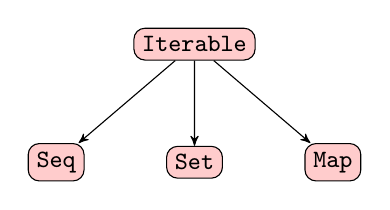
\begin{tikzpicture}[sibling distance=5.0em,->,>=stealth', inner sep=3pt, %scale=0.5,
  every node/.style = {shape=rectangle, draw, align=center,font=\small\ttfamily},
  class/.style = {fill=blue!20},
  trait/.style = {rounded corners, fill=red!20}]
  \node[trait] {Iterable}
      child { node[trait] {Seq} }
      child { node[trait] {Set} }
      child { node[trait] {Map} }
  ;
\end{tikzpicture}

\columnbreak

{\SlideFontTiny

\code{Iterable} har metoder som är implementerade med hjälp av: \\
\code{def foreach[U](f: Elem => U): Unit}\\
\code{def iterator: Iterator[A] }

}

\begin{itemize}\SlideFontTiny
\item[] \code{Seq}: ordnade i sekvens
\item[] \code{Set}: unika element
\item[] \code{Map}: par av (nyckel, värde)
\end{itemize}


\end{multicols}

{\SlideFontSmall Samlingen \Emph{\texttt{Vector}} är en \code{Seq} som är en \code{Iterable}. \\ \vspace{0.5em}%\pause
De konkreta samlingarna är uppdelade i dessa paket:\\
\code{scala.collection.immutable} \hfill där flera är \Emph{automatiskt} importerade\\
\code{scala.collection.mutable}  \hfill som \Alert{måste importeras} explicit\\%\pause
(undantag: primitiva förändringsbara \code{scala.Array} är automatiskt synlig)
}
\end{Slide}




\begin{Slide}{Metoden \texttt{iterator} ger en ''engångs-iterator''}\SlideFontSmall
Med \code{iterator} kan man iterera med \code{while}, men endast \Alert{en   gång}; sedan är iteratorn ''förbrukad''. (Men man kan be om en ny.) Används ''under huven'' i samlingsbiblioteket för att implementera andra metoder.
\begin{REPL}
scala> val xs = Vector(1,2,3,4)
val xs: Vector[Int] = Vector(1, 2, 3, 4)

scala> val it = xs.iterator
val it: Iterator[Int] = <iterator>

scala> while it.hasNext do print(it.next)
1234

scala> it.hasNext
val res0: Boolean = false

scala> it.next
java.util.NoSuchElementException: next on empty iterator
\end{REPL}
\Emph{Normalt} behöver man \Alert{inte} använda \code{iterator}: det finns oftast färdiga metoder som gör det man vill, till exempel \code{foreach}, \code{map}, \code{sum}, \code{min} etc.
\end{Slide}




% \ifkompendium
% \else
% \begin{Slide}{Hierarki av samlingar i scala.collection v2.12}\SlideFontTiny
% \includegraphics[width=0.6\textwidth]{../img/collection/collection-traits}\\
% %\noindent Läs mer om Scalas samlingar här: \\
% \url{https://docs.scala-lang.org/overviews/collections/overview.html}
% \end{Slide}
% \fi



\begin{Slide}{Mer specifika samlingstyper i \texttt{scala.collection}}
Det finns \Alert{mer specifika} \Emph{subtyper} av \code{Seq}, \code{Set} och \code{Map}:
\\ \vspace{1em}

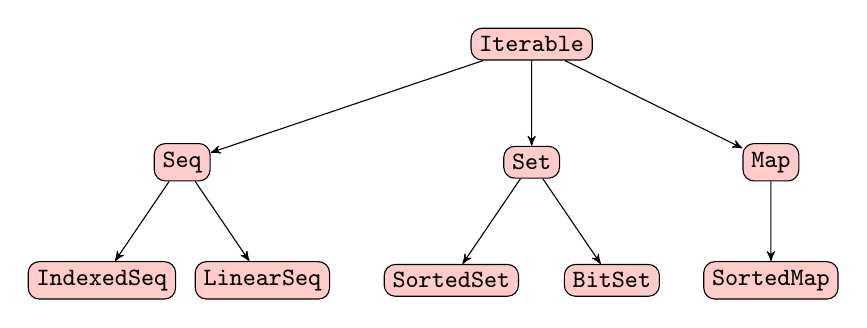
\begin{tikzpicture}[sibling distance=5.8em,->,>=stealth', inner sep=3pt, %scale=0.5,
  every node/.style = {shape=rectangle, draw, align=center,font=\small\ttfamily},
  class/.style = {fill=blue!20},
  trait/.style = {rounded corners, fill=red!20}]
  \node[trait] {Iterable}
      child { node[trait, xshift=-2.4cm] {Seq}
        child { node[trait] {IndexedSeq} }
        child { node[trait] {LinearSeq} }
       }
      child { node[trait, yshift=-0.0cm] {Set}
        child { node[trait] {SortedSet} }
        child { node[trait] {BitSet} }
      }
      child { node[trait, xshift=1.0cm] {Map}
        child { node[trait] {SortedMap} }
    };
\end{tikzpicture}

\pause\vspace{0.5em}
\Emph{\texttt{Vector}} är en \Alert{\texttt{IndexedSeq}} medan
\Emph{\texttt{List}} är en \Alert{\texttt{LinearSeq}}.

\vspace{1em}{\SlideFontSmall
\href
{https://docs.scala-lang.org/overviews/collections-2.13/overview.html}
{docs.scala-lang.org/overviews/collections-2.13/overview.html}
}
\end{Slide}

\begin{Slide}{Några oföränderliga och förändringsbara sekvenssamlingar}\SlideFontSmall
\begin{tabular}{r l l}
\texttt{scala.collection.\Emph{immutable}.Seq.} & & \\
 & \code|IndexedSeq.| & \\
 & & \Emph{\texttt{Vector}} \\
 & & \Emph{\texttt{Range}} \\
 & \code|LinearSeq.| & \\
 & & \Emph{\texttt{List}} \\
   & & \Emph{\texttt{Queue}} \\

\texttt{scala.collection.\Alert{mutable}.Seq.} & & \\
 & \code|IndexedSeq.| & \\
 & & \Alert{\texttt{ArrayBuffer}} \\
 & & \Alert{\texttt{StringBuilder}} \\
 & \code|LinearSeq.| & \\
 & & \Alert{\texttt{ListBuffer}} \\
   & & \Alert{\texttt{Queue}} \\
\end{tabular}

{\SlideFontTiny Fördjupning: Studera samlingars prestanda-egenskaper här:\\ \href{https://docs.scala-lang.org/overviews/collections-2.13/performance-characteristics.html}{docs.scala-lang.org/overviews/collections-2.13/performance-characteristics.html}}
\end{Slide}



\begin{Slide}{Några användbara metoder på samlingar}\SlideFontTiny
\begin{tabular}{r r l}\hline
\texttt{\Emph{Iterable}}
  & \code|xs.size| & antal elementet \\
  & \code|xs.head| & första elementet \\
  & \code|xs.last| & sista elementet \\
  & \code|xs.take(n)| & ny samling med de första n elementet \\
  & \code|xs.drop(n)| & ny samling utan de första n elementet \\
  & \code|xs.foreach(f)| & gör \code|f| på alla element, returtyp \code|Unit|\\
  & \code|xs.map(f)| & gör \code|f| på alla element, ger ny samling \\
  & \code|xs.filter(p)| & ny samling med bara de element där p är sant\\
  & \code|xs.groupBy(f)| & ger en \code|Map| som grupperar värdena enligt f\\
  & \code|xs.mkString(",")| & en kommaseparerad sträng med alla element\\ 
  & \code|xs.zip(ys)| & ny samling med par (x, y); ''zippa ihop'' xs och ys \\
  & \code|xs.zipWithIndex| & ger en \code|Map| med par (x, index för x) \\
  & \code|xs.sliding(n)| & ny samling av samlingar genom glidande ''fönster''\\ \hline

\texttt{\Emph{Seq}}
  & \code|xs.length| & samma som \code|xs.size| \\
  & \code|xs :+ x| & ny samling med x sist efter xs \\
  & \code|x +: xs| & ny samling med x före xs \\ \hline

\end{tabular}
Prova fler samlingsmetoder ur snabbreferensen: ~~\url{http://cs.lth.se/quickref}

\vspace{0.25em}\Emph{Minnesregel} för \code{+:} och \code{:+  } \Alert{Colon on the collection side}\\Digga denna: \url{https://youtu.be/Lm9JWlEMHjo?si=sNdn_ZDaORlGr3lt}

\end{Slide}



% \ifkompendium\else

% \begin{Slide}{scala.collection.immutable}
% \includegraphics[width=0.67\textwidth]{../img/collection/collection-immutable}~~%
% \includegraphics[width=0.3\textwidth]{../img/collection/collection-legend}
% \end{Slide}


% \begin{Slide}{scala.collection.mutable}
% \includegraphics[width=1.05\textwidth]{../img/collection/collection-mutable}
% \end{Slide}

% \fi



% \begin{Slide}{\texttt{Vector} eller \texttt{List}?}\SlideFontTiny
% {\href{http://stackoverflow.com/questions/6928327/when-should-i-choose-vector-in-scala}{stackoverflow.com/questions/6928327/when-should-i-choose-vector-in-scala}}
%
% \begin{enumerate}
% \item If we only need to transform sequences by operations like map, filter, fold etc: basically it does not matter, we should program our algorithm generically and might even benefit from accepting parallel sequences. For sequential operations List is probably a bit faster. But you should benchmark it if you have to optimize.
%
% \item If we need a lot of random access and different updates, so we should use vector, list will be prohibitively slow.
%
% \item If we operate on lists in a classical functional way, building them by prepending and iterating by recursive decomposition: use list, vector will be slower by a factor 10-100 or more.
%
% \item If we have an performance critical algorithm that is basically imperative and does a lot of random access on a list, something like in place quick-sort: use an imperative data structure, e.g. ArrayBuffer, locally and copy your data from and to it.
% \end{enumerate}
% {\href{http://stackoverflow.com/questions/20612729/how-does-scalas-vector-work}{stackoverflow.com/questions/20612729/how-does-scalas-vector-work}}\\
% Mer om tids- och minneskomplexitet i fördjupningskursen och senare kurser.
% \end{Slide}








\Subsection{Repetition: sekvens}

\begin{Slide}{Repetition: Vad är en sekvens?}
\begin{itemize}
\item En sekvens är en \Emph{följd av element} som
  \begin{itemize}
   \item är \Alert{numrerade} (t.ex. från noll), och
   \item är av en viss \Alert{typ} (t.ex. heltal).
  \end{itemize}
  \pause
\item En sekvens kan innehålla \Alert{dubbletter}.
\item En sekvens kan vara \Alert{tom} och ha längden noll.
\item Exempel på en icke-tom sekvens med dubbletter:
\begin{REPLnonum}
scala> val xs = Vector(42, 0, 42, -9, 0, 13, 7)
val xs: Vector[Int] = Vector(42, 0, 42, -9, 0, 13, 7)
\end{REPLnonum}
\pause
\item \Emph{Indexering} ger ett element via dess ordningsnummer:
\begin{REPL}
scala> xs(2)
val res0: Int = 42

scala> xs.apply(2)
val res1: Int = 42
\end{REPL}
\end{itemize}
\end{Slide}


\begin{Slide}{En sträng är också en \texttt{IndexedSeq[Char]}}\SlideFontSmall
Det sker vid behov \Emph{implicit konvertering} från \code{String} till \code{IndexedSeq[Char]}.
\begin{REPLnonum}
scala> val x: IndexedSeq[Char] = "hej"
val x: IndexedSeq[Char] = hej
\end{REPLnonum}

Detta gör att \Alert{alla samlingsmetoder på \texttt{Seq} även funkar på strängar} och även flera andra smidiga strängmetoder erbjuds \Alert{utöver} de som finns i \href{https://www.scala-lang.org/api/current/scala/collection/StringOps.html}{\code{java.lang.String}} genom klassen \href{http://www.scala-lang.org/api/current/scala/collection/immutable/StringOps.html}{\code{StringOps}}.

\vspace{0.5em}
\begin{REPLnonum}
scala> "hej".  //tryck på TAB och se alla strängmetoder
JLine: do you wish to see all 248 possibilities (42 lines)?
\end{REPLnonum}
Detta är en stor fördel med Scala jämfört med många andra språk, som har strängar som inte kan allt som andra sekvenssamlingar kan.
\end{Slide}
  

\begin{Slide}{Konvertera mellan olika samlingstyper}
\begin{itemize}
\item För vanligt förekommande konverteringar finns metoderna \code{toVector}, \code{toList},  \code{toArray}, \code{toBuffer}, \code{toMap}, \code{toSeq}, \code{toIndexedSeq}, \code{toSet},  \code{toString}
\item Metoden \texttt{to} (ny från Scala 2.13) tar ett \Emph{kompanjonsobjekt} ur samlingsbiblioteket som argument och kan användas för konvertering till godtycklig samlingstyp.
\item Detta kräver kopiering om underliggande representation är olika och samlingen är förändringsbar.
\item Kan användas för att t.ex. konvertera mellan oföränderlig och förändringsbar samling:
\end{itemize}
\begin{REPLnonum}
scala> val ms = Set(1,2,3).to(collection.mutable.Set)
val ms: scala.collection.mutable.Set[Int] = HashSet(1, 2, 3)
\end{REPLnonum}
\end{Slide}


\Subsection{Mängd} %%%%%%%%%%%%%%%%%%%%%%%%%%%%%%%%%%%%%%%%%%%%%%%%%%%%%%


\begin{Slide}{Vad är en mängd?}\SlideFontSmall
\begin{itemize}
\item En \Emph{mängd} är en samling \Alert{unika} element av en viss \Alert{typ}.
\item En mängd kan alltså inte innehålla dubbletter:
\begin{REPLnonum}
scala> Set(1,1,2,2,3,3,4,4,5,5)
val res0: Set[Int] = HashSet(5, 1, 2, 3, 4)
\end{REPLnonum}
\pause
\item En mängd är \Alert{inte}  en sekvens: du kan inte utgå från att elementen ligger i någon viss ordning, t.ex. den ordning som de ges vid konstruktion; en mängd har ej längd, men en \Emph{storlek}; metoden \code{size} ger antalet element men metoden \code{length} saknas.
\item En mängd kan vara \Alert{tom} och har då storleken \code{0}.
\pause
\item Man kan gå igenom element i \Emph{någon} ordning (exakt vilken är ej def.), med till exempel \code{xs.map(f)} eller \code{for (x <- xs) yield f(x)}
\pause
\item Det går \Alert{inte} att indexera i en mängd med \code{apply}, som i stället ger \Emph{innehållstest}: \code{Set(1,2,3).apply(3) == true}
\item En mängd \code{Set[T]} med element av typen \code{T} kan således ses som ett \Emph{predikat för innehållstest}: alltså en funktion \code{T => Boolean} som är \code{true} om elementet finns annars \code{false}
\end{itemize}
\end{Slide}


\begin{Slide}{Oföränderlig mängd}
\setlength{\leftmargini}{1em}
\begin{itemize}
\item \Emph{Skapa}:
\begin{REPLnonum}
scala> var xs = Set("gurka", "tomat", "banan", "pingvin")
\end{REPLnonum}

\item \Emph{Läsa}: avgöra medlemskap
\begin{REPLnonum}
scala> xs("gurka")
val res1: Boolean = true
\end{REPLnonum}

\item \Emph{Uppdatera}: lägg till element (händer inget om redan finns)
\begin{REPLnonum}
scala> xs = xs + "jordekorre" // en ny, delvis förändrad
\end{REPLnonum}

\item \Emph{Ta bort}: (om finns, annars händer inget)
\begin{REPLnonum}
scala> xs = xs - "gurka" // en ny, delvis förändrad
\end{REPLnonum}
\end{itemize}
{\SlideFontTiny\code{SLUT} = Skapa, Läsa, Uppdatera, Ta bort \hfill\code{CRUD} = Create, Read, Update, Delete}
\end{Slide}


\begin{Slide}{Mysteriet med de försvunna elementen}
Vad händer här?
\begin{REPLnonum}
scala> val xs1 = Vector(1,2,3,4,5,6)
scala> xs1.map(_ % 2).count(_ == 0)
val res0: Int = 3                          // antalet jämna tal
scala> val xs2 = Set(1,2,3,4,5,6)
scala> xs2.map(_ % 2).count(_ == 0)
val res1: Int = 1                          // varför?
\end{REPLnonum}
\pause
Mängdegenskaper ger att \code{xs2.map(_ % 2) == Set(0, 1)}\\
Fundera alltid noga på om du \Alert{riskerar att förlora duplikat} som du egentligen hade velat behålla!\\
\pause
Använd \code{toSeq} på mängd om du behöver sekvensegenskaper:
\begin{REPLnonum}
scala> xs2.toSeq.map(_ % 2).count(_ == 0)
val res1: Int = 3         // med toSeq blir det som vi ville
\end{REPLnonum}

\end{Slide}
  
  




\begin{Slide}{Förändringsbar mängd}\SlideFontSmall
Med en \Alert{förändringsbar} mängd kan man stegvis utöka på plats.
\begin{REPL}
scala> val mängd = scala.collection.mutable.Set.empty[Int]

scala> for i <- 1 to 1_000_000 do mängd.addOne(i)

scala> mängd.contains(-1)   // samma som mängd(-1) eller mängd.apply(-1)
\end{REPL}
En \Emph{mängd} är \Alert{snabb} på att avgöra om ett element \Alert{finns eller inte} i mängden. Ingen linjärsökning krävs eftersom den smarta implementationen av datastrukturen medger snabb uppslagning \Eng{lookup} av ett element.
\pause
\\\vspace{0.5em}Men i en sekvens krävs linjärsökning vid innehållstest:
\begin{REPL}
scala> val sekvens = (1 to 1_000_000).toVector

scala> sekvens.contains(-1)   // kräver linjärsökning ända till slutet
\end{REPL}
\pause\SlideFontTiny Övning: Testa själv att mäta tidsskillnaden med hjälp av:
\begin{Code}
def nanos(b: => Unit) = { val t0 = System.nanoTime; b; System.nanoTime - t0 }
\end{Code}

\end{Slide}


\begin{Slide}{Speciella metoder på förändringsbar mängd}\SlideFontSmall
Förändringsbara mängder har metoder som ändrar på plats:
\begin{REPLsmall}
scala> val s = scala.collection.mutable.Set.empty[Int]

scala> s.addOne(1)     // finns även under namnet += om du gillar operator-notion
val res0: scala.collection.mutable.Set[Int] = HashSet(1)

scala> s.addOne(2).addOne(3).addOne(3).addOne(42) // addOne returnerar this
val res1: scala.collection.mutable.Set[Int] = HashSet(1, 2, 3, 42)

scala> res0.eq(res1)  // samma instans av mutable.Set (ingen ny har skapats)
val res2: Boolean = true

scala> s.addAll(Vector(3, 4, 5))  // finns även ++= om du gillar operator-notion
val res3: scala.collection.mutable.Set[Int] = HashSet(1, 2, 3, 4, 5, 42)

scala> s.subtractOne(1).subtractAll(List(1,2,3))  // finns även -= och --=
val res4: scala.collection.mutable.Set[Int] = HashSet(4, 5, 42)

scala> s.filterInPlace(_ > 4)
val res5: scala.collection.mutable.Set[Int] = HashSet(5, 42)

\end{REPLsmall}
\code{addOne}, \code{addAll}, \code{subtractOne}, \code{subtractAll}, \code{filterInPlace} returnerar \code{this} så du kan ändra på plats med kedjade anrop med punktnotation.
\end{Slide}

  




\Subsection{Nyckel-värde-tabell} %%%%%%%%%%%%%%%%%%%%%%%%%%%%%%%%%%%%%%%%


\begin{Slide}{Vad är en nyckel-värde-tabell?}\SlideFontSmall
\begin{itemize}
\item En \Emph{nyckel-värde-tabell} är en samling element som är \Alert{par} med:\\
en \Emph{nyckel} av någon typ \code{K} och ett \Emph{värde} av någon typ \code{V}.
\item En sådan tabell kan skapas ur en sekvens av par \code{(k, v)}\\
där \code{k} är en nyckel och \code{v} är ett värde:
\begin{REPL}
scala> val ålder = Map("Björn" -> 42, "Sandra" -> 35, "Kim" -> 19)
val ålder: Map[String, Int] = Map(Björn -> 42, Sandra -> 35, Kim -> 19)
\end{REPL}
\item Tabellens nycklar utgör en mängd som ges av metoden \code{keySet};\\
nycklarna är \Alert{unika}.
\item Elementen utgör \Alert{inte en sekvens} och har ingen speciell ordning;
\\en nyckel-värde-tabell har ej längd, men en \Emph{storlek};\\metoden \code{size} ger antalet element.
\pause
\item En tabell kan ses som en uppslagsfunktion \Eng{dictionary}:\\alltså en funktion \code{K => V} som ger ett värde givet en nyckel.
\end{itemize}
\end{Slide}


\begin{Slide}{Den fantastiska nyckel-värde-tabellen \texttt{Map}}\SlideFontSmall
\begin{itemize}
\item En \Emph{nyckel-värde-tabell} \Eng{key-value table} är en slags generaliserad vektor där man kan ''indexera'' med godtycklig typ.

\item Kallas även \href{https://sv.wikipedia.org/wiki/Hashtabell}{\Emph{hashtabell}} \Eng{hash table}, \Emph{lexikon} \Eng{Dictionary} eller \Emph{mapp} \Eng{Map} (det blir lätt sammanblandning med metoden \code{map}).

\item Om man vet nyckeln kan man slå upp värdet \Alert{snabbt}, på liknande sätt som indexering sker snabbt i en vektor givet heltalsindex.

\item Denna datastruktur är \Alert{mycket användbar} och fungerar som en slags databas i kombination med filtrering, registrering, etc.
\end{itemize}
\end{Slide}


\begin{Slide}{Oföränderlig nyckel-värde-tabell}
\setlength{\leftmargini}{1em}
\begin{itemize}
\item \Emph{Skapa}: ge par till metoden \code{apply} 
\begin{REPLsmall}
scala> var födelse = Map("C" -> 1972,  "C++" -> 1983, "C#" -> 2000,
  "Scala" -> 2004, "Java" -> 1995, "Javascript" -> 1995, "Python" -> 1991)
\end{REPLsmall}

\item \Emph{Läsa}: slå upp ett värde med hjälp av en nyckel
\begin{REPLsmall}
scala> val year = födelse.apply("Scala")
val year: Int = 2004
\end{REPLsmall}

\item \Emph{Uppdatera}: lägga till ett par, ersätta ett par
\begin{REPLsmall}
scala> födelse = födelse + ("Kotlin" -> 2011)
födelse: Map[String, Int] = HashMap(Scala -> 2004, C# -> 2000, Python -> 1991, 
Javascript -> 1995, C -> 1972, C++ -> 1983, Kotlin -> 2011, Java -> 1995)
\end{REPLsmall}

\item \Emph{Ta bort} ett par via nyckeln (om finns, annars händer inget)
\begin{REPLsmall}
scala> födelse = födelse - "Python"
födelse: Map[String, Int] = HashMap(Scala -> 2004, C# -> 2000, 
Javascript -> 1995, C -> 1972, C++ -> 1983, Kotlin -> 2011, Java -> 1995)
\end{REPLsmall}
\end{itemize}
\end{Slide}


\begin{Slide}{Fler exempel nyckel-värde-tabell}\SlideFontSmall
Några ofta förekommande metoder på tabeller:
\begin{itemize}
\item \code{xs.keySet} ger en mängd av alla nycklar
\item \code{xs.map(f)} kör funktionen f på alla par (key, value) i \Alert{någon} ordning
\item \code{xs.map((k, v) => k -> f(v))} kör funktionen f på alla \Emph{värden}
\end{itemize}
\begin{REPLsmall}
scala> val färg = Map("gurka" -> "grön", "tomat"->"röd", "aubergine"->"lila")
val färg: Map[String, String] = 
  Map(gurka -> grön, tomat -> röd, aubergine -> lila)

scala> färg("gurka")
val res0: String = grön

scala> färg.keySet
val res1: Set[String] = Set(gurka, tomat, aubergine)

scala> val ärGrönSak = färg.map((k,v) => (k, v == "grön"))
val ärGrönSak: Map[String,Boolean] = 
  Map(gurka -> true, tomat -> false, aubergine -> false)

scala> val baklängesFärg = färg.map((k, v) => k -> v.reverse)
val baklängesFärg: Map[String,String] = 
  Map(gurka -> nörg, tomat -> dör, aubergine -> alil)
\end{REPLsmall}

\end{Slide}

\begin{Slide}{Från sekvens av par till tabell}
\begin{REPL}
scala> val xs = Vector(("Kim",42), ("Pam", 42), ("Kim", 50), ("Pam", 50))
val xs: Vector[(String, Int)] = 
  Vector((Kim,42), (Pam,42), (Kim,50), (Pam,50))

scala> xs.toMap
val res0: Map[String, Int] = 
  Map(Kim -> 50, Pam -> 50) // inga dublettnycklar

scala> val grupperaEfterNamn = xs.groupBy(_._1)
grupperaEfterNamn: Map[String,Vector[(String, Int)]] =
  Map(Kim -> Vector((Kim,42), (Kim,50)), Pam -> Vector((Pam,42), (Pam,50)))

scala> val grupperaEfterÅlder = xs.groupBy(_._2)
grupperaEfterÅlder: Map[Int,Vector[(String, Int)]] =
  Map(50 -> Vector((Kim,50), (Pam,50)), 42 -> Vector((Kim,42), (Pam,42)))
\end{REPL}
\end{Slide}
  
  
\begin{Slide}{Övning: Implementera en \texttt{Multimap}}
\begin{itemize}
\item Om du lägger till ett värde i en \emph{vanlig} \code{Map} så ersätts  värdet:
\begin{REPLsmall}
scala> val m = Map(1 -> 2, 1 -> 3, 2 -> 1, 2 -> 2) 
val m: Map[Int, Int] = Map(1 -> 3, 2 -> 2)   //senaste värdet gäller
\end{REPLsmall}
...men ibland vill vi i stället lagra alla tillagda värden.
\item En \Emph{multimap} är en speciell nyckel-värde-tabell där värdena utgör en samling (ofta en mängd).
\item En multimap samlar alla värden som har samma nyckel.
\begin{REPL}
  scala> val mm = Multimap(1 -> 2, 1 -> 3, 2 -> 1, 2 -> 2) 
  val mm: Multimap[Int, Int] = Multimap(1 -> Set(2, 3), 2 -> Set(1, 2))
\end{REPL}
\end{itemize}
Övning: Implementera en multimap som fungerar som ovan, med hjälp av en case-klass med attributet \code{toMap} som är en oföränderlig nyckel-värde-tabell där värdena är en mängd. \\Tips: Använd~\code{groupBy}
\end{Slide}

\begin{Slide}{Lösning: \texttt{Multimap}}
\begin{CodeSmall}
case class Multimap[K, V] private (toMap: Map[K,Set[V]]):
  def apply(k: K): Set[V] = toMap(k)
  
  def +(kv: (K, V)): Multimap[K, V] = kv match 
    case (k, v) if toMap.isDefinedAt(k) => Multimap(toMap.updated(k, toMap(k) + v))
    case (k, v) => Multimap(toMap + (k -> Set(v)))
  
  override def toString = toMap.mkString("Multimap(",", ",")")

object Multimap:
  def apply[K, V](kvs: (K,V)*): Multimap[K, V] = 
    new Multimap(kvs.groupBy(_._1).map((k,xs) => k -> xs.map(_._2).toSet))
\end{CodeSmall}
\end{Slide}


\begin{Slide}{Speciella metoder på förändringsbar tabell}\SlideFontSmall
Både \code{Set} och \code{Map} finns i \Alert{förändringsbara} varianter med extra metoder för uppdatering av innehållet ''på plats'' utan att nya samlingar skapas.
\begin{REPLsmall}
scala> import scala.collection.mutable
scala> val ms = mutable.Set.empty[Int]
val ms: scala.collection.mutable.Set[Int] = HashSet()

scala> ms += 42  // metoden += gör samma som addOne
val res0: scala.collection.mutable.Set[Int] = HashSet(42)

scala> ms ++= Seq(1, 2, 3, 1, 2, 3)  // metoden ++= gör samma som addAll 
val res1: scala.collection.mutable.Set[Int] = HashSet(1, 2, 3, 42)

scala> val mm = mutable.Map.empty[String, String]

scala> mm.addOne("hej" -> "svejs").addAll(Seq("abra" -> "kadabra", "ada" -> "lovelace"))
val res2: scala.collection.mutable.Map[String, String] = 
  HashMap(hej -> svejs, abra -> kadabra, ada -> lovelace

scala> mm("abra")
val res3: String = kadabra
\end{REPLsmall}
Metoden \code{++=} gör samma som addAll, används gärna med operator-notation:\\
\code{mm ++= Seq("hej" -> "san", "abra" -> "kada", "bra" -> "scala")}
\end{Slide}
  

\Subsection{Tips inför veckans uppgifter}



\begin{Slide}{Övning: Förändringsbar lokalt, returnera oföränderlig}
\SlideFontSmall
Om du vill implementera en imperativ algoritm med en föränderlig samling:\\
Gör gärna detta \Alert{lokalt} i en \Alert{förändringsbar} samling och returnera sedan en \Emph{oföränderlig} samling, genom att köra t.ex. \code{toSet} på en mängd, eller \code{toMap} på en hashtabell, eller \code{toVector} på en \code{ArrayBuffer} eller \code{Array}.\\~\\
Exempel där lösningen har nytta av lokal förändring på plats:
\begin{Code}
def kastaTärningTillsAllaUtfallUtomEtt(sidor: Int = 6): (Int, Set[Int]) = ???
\end{Code}
\begin{REPL}
scala> kastaTärningTillsAllaUtfallUtomEtt()
val res0: (Int, Set[Int]) = (13,HashSet(5, 1, 6, 2, 3))
\end{REPL}
\end{Slide}


\begin{Slide}{Övning: Förändringsbar lokalt, returnera oföränderlig}
\SlideFontSmall
Om du vill implementera en imperativ algoritm med en föränderlig samling:\\
Gör gärna detta \Alert{lokalt} i en \Alert{förändringsbar} samling och returnera sedan en \Emph{oföränderlig} samling, genom att köra t.ex. \code{toSet} på en mängd, eller \code{toMap} på en hashtabell, eller \code{toVector} på en \code{ArrayBuffer} eller \code{Array}.
\begin{Code}
def kastaTärningTillsAllaUtfallUtomEtt(sidor: Int = 6): (Int, Set[Int]) = 
  /* 
    låt s vara en tom förändringsbar heltalsmängd
    låt n vara noll
    så länge mängden s är mindre än sidor - 1 gör:
      lägg till ett nytt tärningskast i s
      uppdatera n så att vi räknar hur många slumptal som dragits
  */
  (n, s.toSet)   // notera toSet som ger oföränderlig mängd
\end{Code}
\begin{REPL}
scala> kastaTärningTillsAllaUtfallUtomEtt()
val res0: (Int, Set[Int]) = (13,HashSet(5, 1, 6, 2, 3))
\end{REPL}
\end{Slide}


\begin{Slide}{Lösning: Förändringsbar lokalt, returnera oföränderlig}
\SlideFontSmall
Om du vill implementera en imperativ algoritm med en föränderlig samling:\\
Gör gärna detta \Alert{lokalt} i en \Alert{förändringsbar} samling och returnera sedan en \Emph{oföränderlig} samling, genom att köra t.ex. \code{toSet} på en mängd, eller \code{toMap} på en hashtabell, eller \code{toVector} på en \code{ArrayBuffer} eller \code{Array}.
\begin{Code}
def kastaTärningTillsAllaUtfallUtomEtt(sidor: Int = 6): (Int, Set[Int]) = 
  val s = scala.collection.mutable.Set.empty[Int] //förändringsbar lokalt
  var n = 0
  while s.size < sidor - 1 do
    s += util.Random.nextInt(sidor) + 1 
    n += 1
  (n, s.toSet)   // notera toSet som ger oföränderlig mängd
\end{Code}
\begin{REPL}
scala> kastaTärningTillsAllaUtfallUtomEtt()
val res0: (Int, Set[Int]) = (13,HashSet(5, 1, 6, 2, 3))
\end{REPL}
I veckans uppgifter används detta i en s.k. \Emph{builder}: Först bygga upp en förändringsbar struktur i \code{FreqMapBuilder} steg för steg,  
och sedan, då alla tillägg är gjorda, övergå till oföränderlig struktur \code{Map[String, Int]}. 
\end{Slide}


\begin{Slide}{Metoden \texttt{sliding}}\SlideFontSmall
Metoden \code{sliding(n)} skapar med ett ''glidande fönster'' en sekvens av
delsekvenser av längd \code{n} genom att ''svepa fönstret'' från början till slut:
\begin{REPL}
scala> val xs = "fem myror är fler än fyra elefanter".split(' ').toVector
val xs: Vector[String] = Vector(fem, myror, är, fler, än, fyra, elefanter)

scala> xs.sliding(2).toVector
val res0: Vector[Vector[String]] =
  Vector(Vector(fem, myror), Vector(myror, är), Vector(är, fler),
      Vector(fler, än), Vector(än, fyra), Vector(fyra, elefanter))

scala> xs.sliding(3).toVector
val res1: Vector[Vector[String]] =
  Vector(Vector(fem, myror, är), Vector(myror, är, fler),
    Vector(är, fler, än), Vector(fler, än, fyra),
      Vector(än, fyra, elefanter))
\end{REPL}
Denna metod har du nytta av på veckans laboration!
\\(se fler exempel på övning)
\end{Slide}
  
  

\begin{Slide}{Metoderna zipWithIndex, groupBy}
\vspace{-0.5em}
\begin{REPL}
scala> val kort = Vector("Knekt", "Dam", "Kung", "Äss")

scala> val kortIndex = kort.zipWithIndex.toMap
kortIndex: Map[String,Int] = Map(Knekt -> 0, Dam -> 1, Kung -> 2, Äss -> 3)

scala> kortIndex("Kung") > kortIndex("Knekt")
res0: Boolean = true

scala> kortIndex.map(p => p._1 -> (p._2 + 11))

scala> val tärningskast = Vector(1,2,3,4,5,6,2,4,6)

scala> val grupperaStörreÄnFyra = tärningskast.groupBy(_ > 4)
grupperaStörreÄnFyra: Map[Boolean,Vector[Int]] =
  Map(false -> Vector(1, 2, 3, 4, 2, 4), true -> Vector(5, 6, 6))

scala> val grupperaLika = tärningskast.groupBy(x => x)
grupperaLika: Map[Int,Vector[Int]] = Map(5 -> Vector(5), 1 -> Vector(1),
  6 -> Vector(6, 6), 2 -> Vector(2, 2), 3 -> Vector(3), 4 -> Vector(4, 4))

scala> val frekvens = tärningskast.groupBy(x => x).map((k,v) => k -> v.size)
frekvens: Map[Int,Int] = Map(5 -> 1, 1 -> 1, 6 -> 2, 2 -> 2, 3 -> 1, 4 -> 2)

\end{REPL}
\end{Slide}

\begin{Slide}{Fler användbara samlingsmetoder}
Exempel att öva på: räkna bokstäver i ord.  \\
Undersök vad som händer i REPL:
\begin{Code}[basicstyle=\SlideFontSize{9}{13}\ttfamily]
val ord = "sex laxar i en laxask sju sjösjuka sjömän"
val uppdelad = ord.split(' ').toVector
val ordlängd = uppdelad.map(_.length)
val ordlängdMap = uppdelad.map(s => (s, s.size)).toMap
val grupperaEfterFörstaBokstav = uppdelad.groupBy(s => s(0))
val bokstäver = ord.toVector.filter(_ != ' ')
val antalX = bokstäver.count(_ == 'x')
val grupperade = bokstäver.groupBy(ch => ch)
val antal = grupperade.map(p => p._1 -> p._2.size)
//samma som ovan men utnyttjar "parameter untupling":
val antal2 = grupperade.map((k,v) => k -> v.size) 
val sorterat = antal.toVector.sortBy(_._2)
val vanligast = antal.maxBy(_._2)
\end{Code}
%https://dotty.epfl.ch/docs/reference/other-new-features/parameter-untupling.html
\end{Slide}
    
    

%!TEX encoding = UTF-8 Unicode
%!TEX root = ../lect-w09.tex


\Subsection{Serialisering och deserialisering}

\begin{Slide}{Serialisering och deserialisering}
\begin{itemize}
  \item Att \Emph{serialisera} innebär att \Alert{koda objekt} i minnet till en avkodningsbar \Alert{sekvens av symboler}, som kan lagras t.ex. i en fil på din hårddisk.
  \item Att \Emph{de-serialisera} innebär att \Alert{avkoda en sekvens av symboler}, t.ex. från en fil, och \Alert{återskapa objekt} i minnet.
\end{itemize}
\end{Slide}


\begin{Slide}{Läsa text från fil och URL}\SlideFontSmall
I paketet \code{scala.io} finns singelobjektet \code{Source} med metoderna \code{fromFile} och \code{fromUrl} för läsning från fil resp. från  URL, alltså Universal Resource Locator, som börjar t.ex. med \texttt{http://}
\begin{Code}
def läsFrånFil(filnamn: String): String = 
  val s = scala.io.Source.fromFile(filnamn)
  try s.mkString finally s.close // säkerställ stängning även vid krasch

def läsRaderFrånFil(filnamn: String): Vector[String] =
  val s = scala.io.Source.fromFile(filnamn)
  try s.getLines.toVector finally s.close 

def läsFrånWebbsida(url: String): String = 
  val s = scala.io.Source.fromURL(url)
  try s.mkString finally s.close

def läsRaderWebbsida(url: String, kodning: String = "UTF-8"): Vector[String] =
  val s = scala.io.Source.fromURL(url, kodning) // läs med given teckenkodning
  try s.getLines.toVector finally s.close 

\end{Code}
{\SlideFontTiny Se vidare veckans övning. Exempel på annan teckenkodning: \code{"ISO-8859-1"} }
\end{Slide}


\begin{Slide}{Serialisering i modulen \texttt{introprog.IO}}
\begin{itemize}
\item I kursens kodbibliotek \code{introprog} finns ett singelobjekt \code{IO} som samlar smidiga funktioner för serialisering och de-serialisering. 
\item Se api-dokumentation här: \\ \url{https://cs.lth.se/pgk/api/} \\ Sök på IO och klicka på singelobjektet.
\item Se koden här:\\
\url{https://github.com/lunduniversity/introprog-scalalib/blob/master/src/main/scala/introprog/IO.scala}
\item Om du vill får du gärna använda \code{introprog.IO} istället för \code{scala.io.Source} på labben.  
\end{itemize}
\end{Slide}


\input{modules/w10-inheritance-chapter.tex}
\input{modules/w11-context-chapter.tex}
\input{modules/w12-extra-chapter.tex}
\input{modules/w13-examprep-chapter.tex}
\input{modules/w14-extra-chapter.tex}

\part{Appendix}
\appendix
%!TEX encoding = UTF-8 Unicode
%!TEX root = ../compendium2.tex

\chapter{Kojo}\label{appendix:kojo}

\section{Vad är Kojo?}

Kojo%
\footnote{\href{https://en.wikipedia.org/wiki/Kojo_(programming_language)}{en.wikipedia.org/wiki/Kojo\_(programming\_language)}}
 är en integrerad utvecklingsmiljö för Scala som är speciellt anpassad för programmeringsundervisning i grundskolan. Kojo används i LTH:s Science Center Vattenhallen för utbildning av grundskolelärare i programmering och vid skolbesök och annan besöksverksamhet, i vilken lärare och studenter vid LTH arbetar som handledare. 
 
 Kojo är öppen källkod och utvecklingsgemenskapen leds av Lalit Pant från Indien. I Kojo finns även lättillgängliga bibliotek som gör tröskeln lägre att programmera rörlig grafik och enkla spel.

Under kursens första laboration använder vi grafikbiblioteket i Kojo för att illustrera grundläggande begrepp, så som sekvens, alternativ, repetition och abstraktion.  


\begin{figure}[H]
\centering
\includegraphics[width=0.8\textwidth]{../img/kojo/kojo.png}
\caption{Den nybörjarvänliga utvecklingsmiljön Kojo för Scala på svenska.}
\label{fig:appendix:ide:kojo}
\end{figure}

\section{Använda grafikbiblioteket i Kojo}\label{appendix:ide:kojo:install}

Kojo bygger på den beprövade pedagogiska idén med sköldpaddsgrafik \Eng{turtle graphics}\footnote{\url{https://en.wikipedia.org/wiki/Turtle_graphics}}, där du skriver program som styr en sköldpadda med en penna under magen. När sköldpaddan rör sig bildas ett streck av valfri färg på skärmen. Beroende på hur du bestämmer att sköldpaddan ska röra sig och vilken färg du bestämmer att pennan ska ha, kan du skapa olika intressanta bilder och samtidigt lära dig om programmeringens grunder.

Under kursens första laboration ska du använda grafikbiblioteket i Kojo tillsammans med editorn VS \code{code} och \code{scala-cli} i terminalen (se appendix \ref{appendix:terminal} och \ref{appendix:compile}). Ladda ner filen \texttt{kojolib.scala} från \url{https://fileadmin.cs.lth.se/kojolib.scala} och spara i en ny katalog med hjälp av din webbläsare, eller via dessa kommandon (notera att det är stora bokstaven \code{O} och inte en nolla i optionen \code{-sLO}):

\begin{REPLnonum}
> mkdir w01-kojo
> cd w01-kojo
> curl -sLO https://fileadmin.cs.lth.se/kojolib.scala
\end{REPLnonum}

Nu kan du starta Scala REPL och rita med Kojo så här:

\begin{REPLnonum}
> scala-cli repl .
Welcome to Scala 3.1.2 (17.0.2, Java OpenJDK 64-Bit Server VM).
Type in expressions for evaluation. Or try :help.
                                                                                                                               
scala> fram; höger; fram; vänster

\end{REPLnonum}

Du kan starta VS \code{code} i aktuellt bibliotek så här:
\begin{REPLnonum}
> code .
\end{REPLnonum}

Skriv nedan progam i VS \code{code} och spara det i samma katalog som den tidigare nedladdade filen, under ett nytt valfritt filnamn, t.ex. \code{rita.scala}:

\begin{Code}
@main def rita = { fram; höger; fram; vänster }
\end{Code}

Kör ditt fristående program med:
\begin{REPLnonum}
> scala-cli run .
\end{REPLnonum}

Du ska nu få upp ett fönster som heter Kojo Canvas med en sköldpadda som ritat två streck. När du stänger fönstret så avslutas programmet. Prova fler sköldpaddsfunktioner enligt tabell \ref{table:kojo:functions}.

I stället för att ladda ned filen \code{kojolib.scala} så kan du placera dess innehåll på lämpligt ställe i ditt program enligt nedan. Observera att raden som börjar med \code{//> using lib} ska vara en enda lång rad utan radbrytningar.%\code{export} gör Kojos kommandon tillgängliga utan prefix:
\lstinputlisting[breaklines=true,basicstyle=\ttfamily\fontsize{9}{11}\selectfont]{../workspace/w01_kojo/kojo.scala}

\noindent Scala-koden för den svenska paddans api finns här: \\
%\href{https://github.com/litan/kojo/blob/master/src/main/scala/net/kogics/kojo/lite/i18n/svInit.scala}{github.com/litan/kojo/blob/master/src/main/scala/net/kogics/kojo/lite/i18n/svInit.scala} \\
\href{https://github.com/litan/kojo-lib/blob/main/src/main/scala/net/kogics/kojo/i18n/Swedish.scala}{github.com/litan/kojo-lib/blob/main/src/main/scala/net/kogics/kojo/i18n/Swedish.scala}


%Kojo kräver (numera) \emph{inte} att \texttt{java} finns på din dator utan kommer med en egen JVM. 
%Eftersom du behöver tillgång till JDK i kursen, är det lika bra att installera hela JDK direkt (och inte bara JRE, så som beskrivs å länken ovan); se vidare hur du gör detta i avsnitt \ref{appendix:compile:install-jdk}.
%\href{http://www.kogics.net/kojo-download}{www.kogics.net/kojo-download}



\section{Kojo Desktop}

Kojo finns som fristående skrivbordsapplikation, kallad Kojo Desktop. Kojo Desktop innehåller en egen editor med syntaxfärgning för Scala, men fungerar ännu så länge bara för Scala 2. En av de synligaste skillnaderna mellan Scala 2 och Scala 3 är att klammerparenteser vid flerradiga funktioner är nödvändiga i Scala 2, medan Scala 3 har valfria klammerparenteser. Så om du använder Kojo Desktop behöver du komma ihåg att omgärda sekvenser av rader som hör ihop med \code|{| och \code|}|. 

Kojo Desktop är förinstallerad på LTH:s datorer och körs igång med terminalkommandot \texttt{kojo} eller via applikationsmenyn.  För instruktioner om hur du installerar Kojo Desktop på din egen dator se här: \href{http://www.lth.se/programmera/installera/}{lth.se/programmera/installera}

När du startar Kojo första gången, välj ''Svenska'' i språkmenyn och starta om Kojo. Därefter fungerar grafikfunktionerna på svenska enligt tabell \ref{table:kojo:functions} på sidan \pageref{table:kojo:functions}. När du startat om Kojo inställt på svenska ser programmet ut ungefär som i figur \ref{fig:appendix:ide:kojo} på sidan \pageref{fig:appendix:ide:kojo}.

Det finns ett antal användbara kortkommando som du hittar i menyerna i Kojo Desktop. Undersök speciellt Ctrl+Alt+Mellanslag som ger autokomplettering baserat på det du börjat skriva.

%\section{Kojo i Webbläsaren}

%En begränsad variant av Kojo finns tillgänglig för programmering direkt i din webbläsare här: \url{http://kojo.lu.se/}

%När du trycker på play-knappen så kompileras din kod på en server till Javascript via ScalaJS och därefter körs Javascript-koden i din webbläsare. 
%Kojo på webben är också ännu så länge begränsad till Scala 2 och kräver att du omgärdar sekvenser av rader som hör ihop med \code|{| och \code|}|.


\section{Mer om Kojo}

I detta dokument finns en enkel introduktion till Kojo: \\ ''Introduction to Kojo'' \url{http://www.kogics.net/kojo-ebooks#intro}

\noindent I tabell \ref{table:kojo:functions}, som fortsätter på efterföljande sidor, finns ett urval av kommando i Kojo på svenska och engelska.

{\small\renewcommand{\arraystretch}{1.4}
\begin{longtable}{@{}p{0.42\textwidth} p{0.55\textwidth}}

\caption{Ett urval av funktioner i Kojo. Se även \href{http://lth.se/programmera}{lth.se/programmera}}\label{table:kojo:functions}\\

\emph{Svenska/Engelska} & \emph{Vad händer?}  \\ \hline
\input{postchapters/kojo-commands.tex}
\end{longtable}
}%end small

%!TEX encoding = UTF-8 Unicode
%!TEX root = ../compendium2.tex

\chapter{Terminalfönster}\label{appendix:terminal}

\section{Vad är ett terminalfönster?}

I ett terminalfönster kan man skriva kommandon som kör program och hanterar filer. När man programmerar använder man ofta terminalkommandon för att kompilera och exekvera sina program.  
 
\subsubsection{Terminal i Linux}

    \begin{figure}[!b]
    \centering
    \includegraphics[width=1.0\textwidth]{../img/linux-terminal.png}
    \caption{Terminalfönster i Ubuntu öppnas med Ctrl+Alt+T.}
    \label{fig:terminal:linux}
    \end{figure}

I Ubuntu trycker du lättast \textbf{Ctrl+Alt+T} eller sök efter ''terminal'' i app-menyn.  Då öppnas ett fönster med en blinkande markör som visar att det är redo att ta emot dina textkommando. Ett exempel på kommando är \texttt{ls} som skriver ut en lista med filer i den aktuella katalogen, så som visas i fig. \ref{fig:terminal:linux}.

Det som visas i ett terminalfönster sköts av ett \textbf{kommandoskal} \Eng{command shell}, som är redo att ta emot kommando efter en prompt som slutar med ett \texttt{\$}-tecken. När du skriver ett kommando och trycker Enter anropar kommandoskalet en kommandotolk som tolkar och utför dina kommandon. Om ett kommando inte kan tolkas, skrivs ett felmeddelande. 

Det finns många användbara kortkommando, varav de viktigaste visas i tabell \ref{fig:terminal:shortcuts}. Det är bra om du lär dig dessa kortkommandon utantill så att ditt arbete i terminalen går snabbt och smidigt.

\begin{table}[H]
\renewcommand{\arraystretch}{1.15}
\begin{tabular}{@{}r | l}
pil upp/ner & bläddra i kommandohistoriken \\
Tab & ''auto-complete'', fyll i resten baserat på vad du skrivit hittills \\
Tab Tab & två tryck på Tab listar flera alternativ, om så finnes \\
Ctrl+A & ''ahead'', flytta markören till början av raden \\
Ctrl+E & ''end'', flytta markören till slutet av raden \\
Ctrl+K & ''kill'', ta bort tecken från markören till radens slut\\
Ctrl+U & ''undo'', ta bort tecken från markören till början av raden \\
Ctrl+Y & ''yank'', sätt in det som senast togs bort\\
Ctrl+Z & ''zleep'', stoppa pågående process, skriv sedan \texttt{bg} för bakgrundskörning\\
Ctrl+L & rensa terminalfönstret\\
Ctrl+D & avsluta kommandoskalet \\
\end{tabular}
    \caption{Viktiga kortkommandon i Linux terminalfönster.}
    \label{fig:terminal:shortcuts}
\end{table}

\noindent Ctrl+C orsakar normalt ett avbrott av pågående process och istället är \emph{paste} kopplat till Shift+Ctrl+C, men om du vill tvärtom att Ctrl+C ska vara ''Copy'' som vanligt för att kopiera markerad text och göra avbrott med Shift+Ctrl+C , så kan du ställa om detta med terminalfönstrets meny ''Edit $\rightarrow$ Keyboard Shortcuts'', eller liknande.



\subsubsection{PowerShell, Cmd och Linux i Microsoft Windows}
Det finns flera olika sätt att köra terminalkommando i Windows:

\begin{itemize}
\item \textbf{Powershell}. I Microsoft Windows finns kommandotolken \textit{Powershell} med speciell kommandosyntax. Den är inte Linux-baserad men det finns alias definierade för några vanliga Linux-kommandon, inkluderat \texttt{ls}, \texttt{cd} och \texttt{pwd}. Du startar Powershell t.ex. genom att trycka på Windows-knappen och skriva \texttt{powershell}. 
Du kan också, medan du bläddrar bland filer, klicka på filnamnsraden överst i filbläddraren och skriva \texttt{powershell} och tryck Enter; då startas Powershell i aktuellt katalog. %Ändra gärna typsnitt och bakgrundsfärg med hjälp av fönstrets menyer, så att det blir lättare för dig att läsa vad som skrivs.

\item \textbf{Cmd}. Det finns även i Windows den ursprungliga, gamla kommandotolken \textit{Cmd} med helt andra kommandon. Till exempel skriver man i Cmd kommandot \texttt{dir} i stället för \texttt{ls} för att lista filer. 

\item \textbf{WSL}. I både Windows 10 och 11 kan du även köra Ubuntu-terminalen med hjälp av Windows Linux Subsystem (WSL), vilket rekommenderas, speciellt om du inte har möjlighet att göra s.k. dual boot\footnote{Läs mer om dual boot här och be gärna någon om hjälp som gjort det förr:\\ \href{https://www.linuxtechi.com/dual-boot-ubuntu-22-04-and-windows-11/}{https://www.linuxtechi.com/dual-boot-ubuntu-22-04-and-windows-11/}}. 




\begin{itemize}[nolistsep]
\item Se vidare här om hur du kan installera WSL under Windows, (WSL2 rekommenderas före WSL1 om din maskin klarar det): 

\url{https://docs.microsoft.com/en-us/windows/wsl/install}

\item Det finns även ett smidigt tillägg till VS Code som heter Remote-WSL som gör att du kan editera filer i Windows som finns i WSL, se vidare här: 

\url{https://code.visualstudio.com/docs/remote/wsl-tutorial}

\end{itemize}

\item \textbf{Windows Terminal}. Den nya Microsoft-appen \textit{Windows Terminal} rekommenderas oavsett om du använder Powershell, Cmd eller WSL. Läs mer här om hur du installerar Windows Terminal: \\
  \url{https://docs.microsoft.com/en-us/windows/terminal/}

\end{itemize}







% \url{https://ubuntu.com/wsl} 

% Läs mer här: \href{https://www.omgubuntu.co.uk/2020/03/windows-10-linux-kernel-update}{www.omgubuntu.co.uk/2020/03/windows-10-linux-kernel-update}



\subsubsection{Terminal i Apple macOS/OS X}


Apple OS X och macOS är Unix-baserade operativsystem. De flesta vanliga terminalkommandon som fungerar i Linux fungerar också under Apple OS X och macOS. Du startar ett terminalfönster i Apples operativsystem genom att klicka på förstoringsglaset uppe till höger, skriva \texttt{terminal}, och trycka Enter.

\section{Vad är en path/sökväg?}\label{terminal:path}

När du skriver ett kommando i terminalen, eller kör vilket program som helst på din dator, behöver operativsystemet identifera i vilken fil programmets maskinkod ligger innan programmet kan köras. 

Lokaliseringen av filer sker med hjälp av en \textbf{sökväg} \Eng{path}, som anger en position i filsystemet. Ofta betraktas filsystemet som ett upp-och-ned-vänt träd, och kallas därför även ''filträdet''. Den ''översta'' positionen kallas ''rot'' \Eng{root} och betecknas med ett enkelt snedstreck \texttt{/}. Kataloger som ligger i kataloger utgör förgreningar i trädet. En sökväg pekar ut vägar genom trädet som behövs för att nå ''löven'', som utgörs av själva filerna.

Du kan se var ett program ligger i Linux med hjälp av kommandot \texttt{which} enligt nedan.\footnote{Skriv \texttt{ gcm ls } i Windows Powershell för motsvarighet till \texttt{ which ls } \\ Eller skriv \texttt{ New-Alias which get-command } för tillgång till kommandot \texttt{which} i Powershell. \\ \href{http://stackoverflow.com/questions/63805/equivalent-of-nix-which-command-in-powershell}{stackoverflow.com/questions/63805/equivalent-of-nix-which-command-in-powershell}} Listan med kataloger i sökvägen avskiljs med snedstreck.
\begin{REPLnonum}
$ which java
/usr/lib/jvm/oracle_jdk8/bin/java
$ which ls
/bin/ls
\end{REPLnonum}

En sökväg kan vara \textbf{absolut} eller \textbf{relativ}. En absolut sökväg utgår från roten och visar hela vägen från rot till destination, t.ex. \texttt{/usr/bin/firefox}, medan en relativ sökväg utgår från aktuellt katalog (där du ''står'') och börjar \textit{inte} med ett snedstreck.

Alla operativsystem håller reda på en mängd olika sökvägar för att kunna hitta speciella filer i filträdet. Dessa sökvägar lagras i s.k. \textbf{miljövariabler} \Eng{environment variables}. Det finns en \textit{speciell} miljövariabel som heter kort och gott \textbf{PATH}, i vilken alla sökvägar till de program finns, som ska vara tillgängliga för din användaridentitet direkt för exekvering genom sina filnamn, \textit{utan} att man behöver ange absoluta sökvägar. 

Du kan i Linux se vad som ligger i din PATH med kommandot \code{ echo $PATH } medan man i Windows Powershell skriver \code{$env:Path} där det bara är första bokstaven som ska vara en versal. I Linux separeras katalogerna i sökvägen med kolon, medan Windows använder semikolon.

Ibland kan du behöva uppdatera din PATH för att program som du installerat och ska bli allmänt tillgängliga. Detta görs på lite olika sätt i olika operativsystem, för Linux se t.ex. här:
\href{http://stackoverflow.com/questions/14637979/how-to-permanently-set-path-on-linux}{stackoverflow.com/questions/14637979/how-to-permanently-set-path-on-linux}

När man anger sökvägar finns några tecken med speciell betydelse:

\begin{tabular}{r  p{0.8\textwidth}}
\code|~| & ''tilde'', din hemkatalog \\
\code|/| & ''slash'', snedstreck anger filträdets rot om det finns i början av sökvägen, men utgör katalogsavskiljare inuti sökvägen \\
\code|.| & en punkt anger aktuell katalog, där du ''står'' \\
\code|..| & två punkter anger ett steg ''upp'' i filträdet \\
\code|"| & omgärda en sökväg med citationstecken, först och sist, om den innehåller annat än engelska bokstäver, t.ex. blanktecken\\
\code|\ | & \textit{backslash+blanktecken} används för att beteckna mellanslag i sökvägar som \textit{inte} omgärdas av citationstecken\\
\end{tabular}

\section{Några viktiga terminalkommando}

I tabell \ref{fig:terminal:commands} finns en lista med några viktiga terminalkommando som är bra att lära sig utantill.

En introduktion till LTH:s datorer med exempel på hur du använder vanliga Linux-kommandon finns i denna skrift \url{http://www.ddg.lth.se/perf/unix/} som används i introduktionsveckan för nybörjare på datateknikprogrammet vid LTH.

På sajten \url{http://ss64.com/} finns en mer omfattande lista med användbara terminalkommando och tillhörande förklaringarför för Linux (Bash), Windows (Powershell, Cmd) och Apple OS X (Bash).  

\begin{table}[H]
\renewcommand{\arraystretch}{1.25}
   
\begin{tabular}{@{}r | l}
\texttt{ls} & lista filer i aktuell katalog (alltså där du ''står'')\\
\texttt{ls} \textit{p}  & lista filer i katalogen  \textit{p} \\
\texttt{ls -A} & lista alla filer i aktuell katalog, även gömda \\
\texttt{man ls} & manual för kommandot \texttt{ls}; testa även \texttt{man} för andra kommandon! \\
\texttt{cd} \textit{p} & ''change directory'', ändra aktuell katalog till \textit{p}\\
\texttt{pwd} & ''print working directory'', skriv ut sökväg för aktuell katalog \\
\texttt{cp} \textit{p1 p2} & ''copy'', kopiera filen med path \textit{p1} till en ny fil kallad \textit{p2} \\
\texttt{mv} \textit{p1 p2} & ''move'', byt namn på filen \textit{p1} till \textit{p2}  \\
\texttt{rm} \textit{p} & ''remove'', ta bort filen \textit{p}\\
\texttt{rm -r} \textit{p} & ''remove recursive'', ta bort katalogen \textit{p} med allt innehåll; var försiktig!\\
\texttt{mkdir} \textit{p} & ''make dir'', skapa ett en katalog \textit{p}\\
\texttt{cat} \textit{p1 p2}& ''concatenate'', skriv ut hela innehållet i en eller flera filer \textit{p1 p2 etc.}\\
\texttt{less} \textit{p}& skriv ut innehållet i filen \textit{p}, en skärm i taget\\
\texttt{wget} \textit{url}&ladda ner \textit{url}, t.ex. \texttt{ wget http://cs.lth.se/pgk/ws -o ws.zip}\\
\texttt{unzip} \textit{p}& packa upp \textit{p}, t.ex. \texttt{ unzip ws.zip}\\
\end{tabular}

    \caption{Några viktiga terminalkommando i Linux. Med \textit{p}, \textit{p1}, \textit{p2}, etc.  avses en absolut eller relativ sökväg \Eng{path}, se avsnitt \ref{terminal:path}.}
    \label{fig:terminal:commands}

\end{table}


%!TEX encoding = UTF-8 Unicode
%!TEX root = ../compendium2.tex

\chapter{Editera, kompilera och exekvera}\label{appendix:compile}

\section{Vad är en editor?}

En editor används för att redigera programkod. Det finns många olika editorer att välja på. Erfarna utvecklare lägger ofta mycket energi på att lära sig att använda favoriteditorns kortkommandon och specialfunktioner, eftersom detta påverkar stort hur snabbt kodredigeringen kan göras.

En bra editor har \textbf{syntaxfärgning} för språket du använder, så att olika delar av koden visas i olika färger. Då går det mycket lättare att läsa och hitta i koden.

Nedan listas några viktiga funktioner som man använder många gånger dagligen när man kodar:

\begin{itemize}
\item \textbf{Navigera}. Det finns flera olika sätt att flytta markören och bläddra genom koden. Alla editorer erbjuder sökmöjligheter, och de flesta editorer har även mer avancerade sökfunktioner där kodmönster kan identifieras och multipla sökträffar markeras över flera kodfiler.

\item \textbf{Markera}. Att markera kod kan göras på många sätt: med piltangenter+Shift, med olika speciella menyalternativ, med mus + dubbelklick eller trippelklick, etc. I vissa editorer finns även möjlighet att ha multipla markörer så att flera rader kan editeras samtidigt.

\item \textbf{Kopiera}. Genom Copy-Paste slipper du du skriva samma sak många gånger. Kortkommandona Ctrl+C för Copy och Ctrl+V för Paste sitter i fingrarna efter ett tag. Man ska dock vara medveten om att det lätt blir fel när man kopierar en stor del som sedan ska ändras lite; många Copy-Paste-buggar kommer av att man inte är tillräckligt noggrann och ofta är det bättre att skriva från grunden i stället för att kopiera så att du hinner tänka efter medan du skriver.

\item \textbf{Klipp ut}. Genom Ctrl+X för Cut och Ctrl+V för Paste, kan du lätt flytta kod. Att skriva kod är en stegvis process där man gör många förändringar under resans gång för att förbättra och vidareutveckla koden. Att flytta på kod för att skapa en bättre struktur är mycket vanligt.

\item \textbf{Formatering}. Med indragningar, radbrytningar och nästlade block i flera nivåer får koden struktur. Många editorer kan hjälpa till med detta och har speciella kortkommandon för att ändra indragningsnivå inåt eller utåt.

\item \textbf{Parentesmatchning}. Olika former av parenteser, \code+ ( { [ ) } ] +,  behöver matchas för att koden ska fungera; annars går kompilatorn ofta helt vilse och konstiga felmeddelanden kan peka på helt fel plats i koden. En bra kodeditor kan hjälpa dig att markera vilka parentespar som hör ihop så att du undviker att spendera för mycket tid med att leta efter en parentes som saknas eller står i vägen.

\end{itemize}

\subsection{Välj editor}\label{appendix:compile:edit}

I tabell \ref{edit:popular-editors} visas en lista med några populära editorer. Det är en stor fördel om din favoriteditor finns på flera plattformar så att du har nytta av dina förvärvade färdigheter när du behöver växla mellan olika operativsystem.

I denna kurs rekommenderas Visual Studio \textbf{\texttt{code}}, eftersom den är öppen, gratis och finns för Linux, Windows och Mac, och har bra stöd för Scala och Java. Men om du redan är van vid någon annan av editorerna i tabell \ref{edit:popular-editors} så fungerar de också bra. 

En integrerad utvecklingsmiljö \Eng{integrated development environment, IDE}, se appendix \ref{appendix:ide}, erbjuder många avancerade funktioner som hjälper dig att koda effektivt när du väl lärt dig handgreppen. VS \texttt{code} har numera flera IDE--funktioner, och gränsen mellan en renodlad editor och en IDE, så som IntelliJ och Eclipse, är inte längre lika tydlig som förr.  %Men även när du lärt dig använda en IDE kommer du fortfarande ha stor nytta av en ''vanlig'' editor. Ofta har man flera terminalfönster igång, tillsammans med flera editorfönster och en IDE.

%Om du jobbar i Linux och hellre vill börja med en enklare editor, kan du prova \texttt{gedit}. När du behöver mer avancerade funktioner kan du gå över till \texttt{code}.

%Det kan vara bra att lära sig de allra mest basala kommandona (starta, spara, ändra text och avsluta) i editorerna \texttt{vim} och \texttt{nano}, eftersom dessa kan köras direkt i terminalen, även vid fjärrinloggning utan fönstersystem, och finns förinstallerade i de flesta Linux-system.


\begin{table}

\renewcommand{\arraystretch}{2.0}\small

    \caption{Några populära editorer. I kursen rekommenderas VS Code.}
    \label{edit:popular-editors}

\begin{longtable}{@{}r | p{0.8\textwidth}}
\textit{Editor} & \textit{Beskrivning} \\ \hline

VS Code & Öppen, fri och gratis. Finns för Linux, Windows, \& Mac. Är förinstallerad på LTH:s Linux-datorer och startas med kommandot \verb+code+. Öppenkällkodsprojektet startades av Microsoft och har en aktiv gemenskap med många utvecklare och många användbara tillägg \Eng{extensions}. Sök efter tillägget \texttt{scalameta.metals} och installera så får du syntaxfärgning och många andra IDE-funktioner för Scala.
\newline \url{https://code.visualstudio.com/} \newline \url{https://scalameta.org/metals/docs/editors/vscode/#installation}\\

Gedit & Öppen, fri och gratis. Lätt att lära men inte så avancerad. Är förinstallerad på LTH:s Linux-datorer och startas med kommandot \verb+gedit+. \newline \url{https://wiki.gnome.org/Apps/Gedit} \\

Nano & Öppen, fri och gratis. En simpel editor för enkla småjobb i terminalen. Är förinstallerad på de flesta Linux-system på planeten Jorden. Startas med kommandot \verb+nano+. \newline \url{https://www.nano-editor.org/}\\

Notepad++ & Öppen, fri och gratis. Utvecklad speciellt för Windows men finns även för Linux. \newline \url{https://notepad-plus-plus.org/} \newline \url{https://snapcraft.io/notepad-plus-plus}\\

Vim & Öppen, fri och gratis. Hög inlärningströskel. Finns för Linux, Windows, \& Mac. Är förinstallerad på LTH:s Linux-datorer och startas med kommandot \verb+vim+. Med Scala Metals (se länk nedan) får du IDE-liknande funktioner. Du avslutar vim genom att trycka Escape och sedan skriva :q och trycka Enter.\newline \url{http://www.vim.org/} \newline \url{https://scalameta.org/metals/docs/editors/vim.html}\\

Emacs & Öppen, fri och gratis. Hög inlärningströskel. Finns för Linux, Windows, \& Mac. Är förinstallerad på LTH:s Linux-datorer och startas med kommandot \verb+emacs+. Med Scala Metals (se länk nedan) får du IDE-liknande funktioner. \newline \url{http://www.gnu.org/software/emacs/} \newline \url{https://scalameta.org/metals/docs/editors/emacs.html}\\

Sublime Text& Sluten källkod. Gratis att prova på, men programmet föreslår då och då att du köper en licens. Finns för Linux, Windows, \& Mac. Med Scala Metals (se länk nedan) får du IDE-funktioner. \newline \url{http://www.sublimetext.com/3} \newline \url{https://scalameta.org/metals/docs/editors/sublime.html} \\



% Textwrangler & Sluten källkod. Gratis. Lätt att lära men inte så avancerad. Finns endast för Mac.
% \newline \url{http://www.barebones.com/products/textwrangler/} \\

\end{longtable}

\end{table}

\section{Vad är en kompilator?}

En \textbf{kompilator} \Eng{compiler} är ett program som läser programtext och översätter den till exekverbar maskinkod, så som visas i figur \ref{fig:appendix:compiler}. Programtexten som kompileras kallas källkod och utgörs av text som följer reglerna för ett programmeringsspråk, till exempel Scala eller Java.

\begin{figure}[H]
\centering
\begin{tikzpicture}[node distance=1.8cm, scale=1.5]
\node (input) [startstop] {\bf\sffamily Källkod};
\node(inptext) [right of=input, text width=2cm, xshift=1.5cm]{För\\människor};
\node (compile) [process, below of=input] {\bf\sffamily Kompilator};
%\node(explain) [right of=compile, text width=5cm, xshift=3.0cm]{Översätter från källkod till maskinkod};
\node (output) [startstop, below of=compile] {\bf\sffamily Maskinkod};
\node(outtext) [right of=output, text width=2cm, xshift=1.5cm]{För\\maskiner};
\draw [arrow] (input) -- (compile);
\draw [arrow] (compile) -- (output);
\end{tikzpicture}
    \caption{En kompilator översätter från källkod till maskinkod.}
    \label{fig:appendix:compiler}
\end{figure}




Vissa kompilatorer genererar kod som kan köras av en processor direkt, medan andra kompilatorer genererar ett mellanformat som tolkas under exekveringen. Det senare är fallet med Java och Scala, vilket möjliggör att programmet kan kompileras en gång för alla plattformar och sedan kan programmet köras på all de processorer till vilka det finns en s.k. virtuell maskin för Java \Eng{Java Virtual Machine, JVM}. Den kod som genereras av en kompilator för JVM kallas \textbf{bytekod}.

Om kompileringen inte lyckas skriver kompilatorn ut ett felmeddelande och ingen maskinkod genereras. Det är inte lätt att bygga en kompilator som ger bra felmeddelanden i alla lägen, men felmeddelandet ger oftast goda ledtrådar till felorsaken efter att man lärt sig tolka det programmeringsspråksspecifika vokabulär som kompilatorn använder.

Även om programmet kompilerar utan felmeddelande och genererar exekverbar maskinkod, är det vanligt att programmet ändå inte fungerar som det är tänkt. Ibland är det mycket svårt att lista ut vad problemet beror på och man kan behöva göra omfattande undersökningar av vad som händer under körningen, genom att t.ex. skriva ut olika variablers värden eller på annat sätt ändra koden och se vad som händer. Denna process kallas felsökning eller avlusning \Eng{debugging}, och är en väsentlig del av all systemutveckling. Läs mer om debugging i Appendix \ref{appendix:debug}.

En uttömmande testning av ett större program, som kör programmets \textit{alla} möjliga exekveringsvägar, är i praktiken omöjlig att genomföra inom rimlig tid, då antalet kombinationsmöjligheter växer mycket snabbt med storleken på programmet.
Därför är kompilatorn ett mycket viktigt hjälpmedel. Med hjälp av den analys och de kontroller som görs av kompilatorn kan många buggar, som annars vore mycket svåra att hitta, undvikas och åtgärdas i kompileringsfasen, redan \textit{innan} man exekverar programmet.


\section{Java JDK}

Scala, Java och flera andra språk använder Java-plattformen som exekveringsmiljö. Om man inte bara vill köra program som andra har utvecklat, utan även utveckla egna program som fungerar i denna miljö, behöver man installera Java Develpment Kit (JDK). Detta utvecklingspaket innehåller flera delar, bland annat:

\begin{itemize}

\item Kompilatorn \texttt{javac} kompilerar Java-program till bytekod som lagras i klassfiler med filnamnsändelsen \texttt{.class}.

\item Exekveringsmiljön Java Runtime Enviroment (JRE) med kommandot \texttt{java} som drar igång den virtuella javamaskinen (Java Virtual Machine) som kan ladda och exekvera bytekod lagrade i klassfiler.

\item Programmet \texttt{jar} som packar ihop många sammanhörande klassfiler till en enda jar-fil som lätt kan distribueras via nätet och sedan köras med \texttt{java}-kommandot på alla maskiner med JRE.

\item Programmet \texttt{javap} som läser klassfiler och skriver ut vad de innehåller i ett format som kan läsas av människor (ett sådant program kallas disassembler).

\item I JDK ingår också en mycket stor mängd färdiga programbibliotek med stöd för nätverkskommunikation, filhantering, grafik, kryptering och en massa annat som behövs när man bygger moderna system.

\end{itemize}

\noindent Du kan läsa mer om Java och dess historik här: \\
\href{https://en.wikipedia.org/wiki/Java_(programming_language)}{https://en.wikipedia.org/wiki/Java\_(programming\_language)}

\subsection{Kontrollera om du har JDK installerat}\label{appendix:compile:check-jdk}

Öppna ett terminalfönster (se appendix \ref{appendix:terminal}) och skriv (observera det avslutande c:et i \texttt{javac}):
\begin{REPLnonum}
javac -version
\end{REPLnonum}
Då ska något som liknar följande skrivas ut, där \texttt{x} och \texttt{y} är siffror:\\
\texttt{javac \JDKVersion.x.y}\\
Om utskriften säger att \texttt{javac} saknas, installera JDK enl. nedan.

Vi använder alltså JDK \JDKVersion~i kursen. Det går också bra att använda de äldre versionerna JDK 8 och JDK 11, men JDK 9 eller 10 fungerar inte med alla verktyg vi använder och senare versioner än \JDKVersion~ kan också ge problem. Läs mer under ''Verktyg'' på kurshemsidan.

%Du kanske redan har enbart Java Runtime Environment (JRE) installerad, men inte JDK. Då saknar du Javakompilatorn \texttt{javac} m.m. och behöver installera JDK, se nedan. Du kan kolla om du har JRE genom att skriva \texttt{java -version} (alltså utan \texttt{c} efter \texttt{java}). Eller så har du redan JDK installerad men inte rätt katalog i din PATH. 





\subsection{Installera JDK}\label{appendix:compile:install-jdk}

Det finns flera JDK-distributioner att välja mellan, varav OpenJDK och Oracle JDK är två exempel. Vi använder OpenJDK i kursen, som kan installeras via \\ \url{https://adoptium.net/temurin/releases/?version=21}. 

Om du installerar alla Scala-verktyg med hjälp av Coursier enligt instruktioner på kurshemsidan under ''Verktyg'', \url{https://lunduniversity.github.io/pgk/#verktyg} så kommer JDK att installeras automatiskt (om du inte redan har JDK). % För att installera JDK på din egen dator behöver du gå igenom flera steg, varav vissa behöver anpassas efter det operativsystem du kör, enligt nedan.

%
%
%
% Din användaridentitet behöver ha administratörsrättigheter för att du ska kunna genomföra installationen.
%
%
%
% \subsubsection{Linux}
% För Ubuntu: läs igenom och följ sedan dessa instruktioner noga: \\ \href{http://www.webupd8.org/2012/09/install-oracle-java-8-in-ubuntu-via-ppa.html}{www.webupd8.org/2012/09/install-oracle-java-8-in-ubuntu-via-ppa.html}
%
% För andra Linux-distributioner, kör detta i terminalen (funkar även i Ubuntu, men du får med detta kommando inte Oracles aningen snabbare JVM): \\ \texttt{sudo apt-get install openjdk-8-jdk}
%
% \subsubsection{Windows/macOS}
%
% \begin{enumerate}
% \item Installera senaste JDK från Oracle. Om du inte har installerat JDK förr på din dator så be gärna någon kurskamrat med erfarenhet av detta att assistera dig medan du följer stegen nedan.
%
% \begin{enumerate}
% \item Surfa till Oracles hemsida för Java SE här: \\ \url{http://www.oracle.com/technetwork/java/javase/downloads/}
%
% \item Klicka på rubriken ''Java SE 8u101 / 8u102'' och på nästa sida klicka på knappen ''Accept License Agreement'' i listan under rubriken ''Java SE Development Kit 8u101''. (Siffrorna 101 eller 102 kan vara annorlunda om senare versioner tillkommit.)
%
% \item Välj rätt version av operativsystem (Windows x64 eller Mac OS X). Det är viktigt att du väljer x64, d.v.s 64-bitarsvarianten som gäller för alla moderna datorer.
%
% \item Klicka på länken och en stor fil kommer laddas ner till din dator.
%
% \item Installera när filen laddats färdigt.
%
% \end{enumerate}
%
% \item Uppdatera PATH, så att du får tillgång till alla kommando i terminalen:
% \begin{itemize}
% \item För Windows görs detta enklast genom att ladda ner och sedan köra denna fil genom att dubbelklicka på den: \\ \mbox{\href{https://github.com/lunduniversity/introprog/raw/master/tools/windows-jdk-set-path.bat}{github.com/lunduniversity/introprog/raw/master/tools/windows-jdk-set-path.bat}}
% \item För macOS, läs här: \\ \href{https://docs.oracle.com/javase/8/docs/technotes/guides/install/mac_jdk.html}{docs.oracle.com/javase/8/docs/technotes/guides/install/mac\_jdk.html}
% \\ Ge bästa rådet att sätta path på mac; HOMEBREW!!!
%
% \item Om något krånglar, be om hjälp. Om du behöver mer detaljer om PATH-uppdatering för java, läs här:  \href{https://java.com/sv/download/help/path.xml}{java.com/sv/download/help/path.xml} \\
% Om du kör engelska menyer byt \texttt{sv} mot \texttt{en} i adressen ovan.  Du kan ta reda på vilken katalog som ska läggas in sist i din PATH genom att bläddra bland dina systemfiler och undersöka var JDK har installerats; i Windows antagligen något liknande detta (kolla exakt vilket versionsnummer du har): \code|C:\Program Files\Java\jdk1.8.0_101\bin|
% \end{itemize}
%
% \item Starta om datorn. Det är först efter att en ny användarinloggning initierats, som PATH-tilldelningen får effekt.
%
% \item Kontrollera att \texttt{javac} fungerar enligt avsnitt \ref{appendix:compile:check-jdk}.
% \end{enumerate}


\section{Scala}

Scala använder Java Virtual Machine (JVM) som exekveringsmiljö, men går även att köra i browsern med hjälp av ScalaJS-kompilatorn som kompilerar från Scala till JavaScript. I denna kurs använder vi i Scala på JVM.
I en Scala-installation ingår bl.a. kompilatorn \texttt{scalac} och även ett interaktivt kommandoskal kallat Scala REPL (se nedan \ref{appendix:compile:REPL}) där du kan testa din Scala-kod rad för rad och se vad som händer direkt.

%De flesta av kursens övningar görs i Scala REPL (förk. \textit{read-evaluate-print-loop}), medan laborationerna kräver kompilering av lite större program.

Den officiella hemsidan för Scala finns här: \url{http://www.scala-lang.org/}

Du hittar mer om Scalas historik och annan bakgrundsinformation här:\\\mbox{%
 \href{https://en.wikipedia.org/wiki/Scala_(programming_language)}{en.wikipedia.org/wiki/Scala\_(programming\_language)}
}

\subsection{Installera Scala}

Scala finns förinstallerat på LTH:s datorer. På kurshemsidan under ''Verktyg'' finns detaljerade instruktioner om hur du installerar Scala på din egen dator:  \\ \url{https://lunduniversity.github.io/pgk/#verktyg}

% \begin{enumerate}
% \item Kontrollera att du har JDK installerad enligt avsnitt \ref{appendix:compile:check-jdk} och installera vid behov enligt avsnitt \ref{appendix:compile:install-jdk}.
% \item Surfa till denna hemsida för nedladdning av Scala 2.11.8: \\ \url{http://scala-lang.org/download/2.11.8.html}
% \item Klicka på ''Download'' av den variant som är relevant för ditt operativsystem och spara filen:
%
% \begin{enumerate}
% \item \textbf{Linux Ubuntu}: Filen heter \texttt{scala-2.11.8.deb} och installeras genom att dubbelklicka på filen eller via terminalkommandot:\\ \code{sudo apt install ~/Downloads/scala-2.11.8.deb} \\ Anpassa sökvägen ovan efter var du sparade filen.
% \item \textbf{Windows}: Filen heter \texttt{scala-2.11.8.msi} och installationen startas med ett dubbelklick. Följ instruktionerna. Installationsprogrammet uppdaterar även din PATH åt dig och kommandot \texttt{scala} bör fungera efter omstart.
% \item \textbf{Mac}: Filen heter \texttt{scala-2.11.8.tgz} och kan packas upp på lämpligt ställe med terminalkommandot \texttt{tar -xvzf scala-2.11.8.tgz} och sedan är det underkatalogen \texttt{bin} som ska inkluderas i din PATH. \TODO klura ut säkraste rådet för PATH-uppdatering på mac -- enklast är nog att visa hur man installerar via homebrew
% \end{enumerate}
% \end{enumerate}
% Kontrollera, efter ev. omstart, att terminalkommandot \texttt{scala} nu kan användas för att starta Scala REPL på din dator:
% \begin{REPLnonum}
% > scala
% Welcome to Scala 2.11.8 (Java HotSpot(TM) 64-Bit Server VM, Java 1.8.0_101).
% Type in expressions for evaluation. Or try :help.
%
% scala> val msg = "hej"
% msg: String = hej
%
% scala> println(msg)
% hej
%
% scala>
% \end{REPLnonum}


\subsection{Scala Read-Evaluate-Print-Loop (REPL)}\label{appendix:compile:REPL}

För många språk, t.ex. Scala och Python, finns det ett interaktivt program ämnat för terminalen som gör det möjligt att exekvera enstaka programrader och direkt se effekten. Ett sådant program kallas \textit{Read-Evaluate-Print-Loop} (REPL), eftersom det läser  och tolkar en rad i taget. Resultatet av evalueringen av din kod skrivs ut i terminalen och därefter är kommandoskalet redo för nästa kodrad.

Kursens övningar bygger till stor del på att du använder Scala REPL för att undersöka principer och begrepp som ingår i kursen genom dina egna kodexperiment. Även när du på labbarna utvecklar större program med en editor och en IDE, är det bra att ha Scala REPL till hands. Då kan du klistra in delar av programmet du håller på att utveckla i Scala REPL och stegvis utveckla delprogram, som till slut fungerar så som du vill.

I Scala REPL får du se typinformation för variabler och metoder, vilket är till stor hjälp när man försöker lista ut vad en kodrad innebär. Genom att öva upp din förmåga att dra nytta av Scala REPL, kommer din produktivitet öka.

Du startar Scala REPL med kommandot \texttt{scala} och skriver Scala-kod efter prompten \texttt{scala>} och kompilering+exekvering sker när du trycker Enter.
\begin{REPLnonum}
> scala
Welcome to Scala 3.1.2 (17.0.2, Java OpenJDK 64-Bit Server VM).
Type in expressions for evaluation. Or try :help.
                                                                                                                               
scala> 41 + 1
val res0: Int = 42
\end{REPLnonum}

Varje evaluerat värde sparas i en ny variabel, här \code{res0}.

Om du skriver en ofullständig rad fortsätter editeringen på nästa rad. Du kan navigera mellan raderna med pil-upp- och pil-ner-tangenterna. När du avslutar med en rad som gör din kod fullständig så kompileras och exekveras alla raderna. Du kan avbryta flerradsediteringen i förtid genom skriva ett semikolon \texttt{;} och sen trycka Enter. Vill du fortsätta editeringen med en ny rad och förhindra för tidig evaluering så tryck Esc+Enter. Escape-tangenten finns överst till vänster på tangentbordet. Se exempel nedan:

\begin{REPLnonum}
scala> def fleraRader = 42  // Esc+Enter ger ny rad
     |   + "ny rad".length  // fortsättningsrad, avsluta med Enter
\end{REPLnonum}

Beroende på vilket operativsystem du kör så kan även andra tangentkombinationer fungera för att starta ny rad i REPL; prova t.ex. Linux: Left Alt+Enter, Windows: Left Alt + Shift + Enter, VS Code Terminal i Windows Left Alt + Enter, VS Code Terminal i MacOS: Option + Enter.

Många av de kortkommandon som fungerar i terminalens kommandoskal, fungerar också i Scala REPL. Gå gärna igenom listan i tabell \ref{fig:terminal:shortcuts} på sidan \pageref{fig:terminal:shortcuts}, och testa vad som händer i Scala REPL. Om du tränar upp din fingerfärdighet med dessa kortkommandon, går ditt arbete i Scala REPL väsentligt snabbare.

Med kommandot \texttt{:help} får du se en lista med specialkommandon för Scala REPL:

\begin{REPLsmall}
The REPL has several commands available:

:help                    print this summary
:load <path>             interpret lines in a file
:quit                    exit the interpreter
:type <expression>       evaluate the type of the given expression
:doc <expression>        print the documentation for the given expression
:imports                 show import history
:reset [options]         reset the repl to its initial state, forgetting all session entries
:settings <options>      update compiler options, if possible


\end{REPLsmall}

Du kan också starta Scala REPL med hjälpa av kommandot \code{scala-cli repl . } ~med ett blanktecken och en punkt på slutet. Punkten gör att alla \code{.scala}-filer som finns i aktuell katalog kompileras av Scala CLI och görs tillgänglig för användning i REPL.  

\subsection{Kompilera och kör med Scala Command Line Interface}\label{appendix:compile:scala-cli}

Det finns sedan 2022 ett nytt smidigt kommandoradsgränssnitt \Eng{command line interface} för att kompilera, exekvera och paketera Scala-program som kallas \emph{Scala CLI}. Om du installerar Scala-verktygen enligt instruktioner på kurshemsidan under ''Verktyg'', \url{https://lunduniversity.github.io/pgk/#verktyg} så medföljer Scala CLI. 

Här finns några användbara kommandon:
\begin{itemize}
\item Första gången du kör en nyinstallerad Scala CLI-installation så kör detta kommando så att du får tillgång till smidiga kompletteringar med TAB-tangenten:\\
\texttt{scala-cli install completions}

\item Med hjälp av detta kommando kan du förbereda VS Code för samverkan med Scala CLI (notera blanktecken och avslutande punkt):\\ 
\texttt{scala-cli setup-ide .}\\
Kör ovan kommando innan du startar VS Code första gången med \texttt{code .} i aktuell katalog, eller avsluta VS Code och kör ovan kommando och starta VS Code igen med \texttt{code .}  i aktuell katalog.


\item Scala CLI kan köra igång REPL i aktuell katalog med dina Scala- och Java-program automatiskt kompilerade och tillgängliggjorda i REPL med hjälp av nedan kommando. Med optionen \code{-S} anger du vilken version av Scala du vill köra:\\
\code{scala-cli repl . -S 3}

\item I stället för att ange Scala-version med optionen \code{-S} på kommandoraden kan du inuti ditt program, på första raden, skriva denna ''magiska'' kommentar:\\ 
\code{//> using scala "3.1.2"} \\
Då kommer Scala CLI att automatiskt välja (och vid behov ladda ned) önskad version av Scala-kompilatorn (notera \code{>} efter \texttt{//}):

\item Kompilera alla Scala- och Java-program i aktuell katalog och se eventuella felmeddelanden. Med hjälp av \code{--watch} (kan förkortas till \code{-w}) så kompileras alla filer automatiskt om så fort ändringar sparas i VS Code (kortkommando Ctrl+S):\\
\code{scala-cli compile . --watch}

\item Kör Scala- och Java-program i aktuell katalog med start av den topp-nivå-\code{def} som är märkt \code{@main} (om det finns flera får du en frågan om vilken \code{@main def} du vill köra).:\\
\code{scala-cli run .}

\item Skapa en exekverbar fil:\\
\texttt{scala-cli package .}

\item Skapa en kopia av ditt projekt med katalogstruktur och filer anpassade för byggverktyget \code{sbt} (se Appendix \ref{appendix:build}):\\
\verb|scala-cli export . --sbt --output ../nameofnewprojdir|\\
Ändra katalognamnet \code{nameofnewprojdir} till valfritt nytt namn på en katalog som inte existerar. Notera de dubbla punkterna som gör att nya katalogen hamnar på samma nivå som ditt nuvarande projekt, och \emph{inte} i din aktuella katalog (för att undvika att dubbletter av dina scala-filer ger kompileringsfel).

\item Om du skriver \texttt{scala-cli help} så får du se vad du mer kan göra.
\end{itemize}


\noindent
Läs mer om Scala CLI i Appendix \ref{appendix:build:scala-cli} och här: \\ \url{https://scala-cli.virtuslab.org/}


% \begin{table}
% \renewcommand{\arraystretch}{1.25}\centering
%     \caption{Några vanliga kommandon i Scala REPL.}
%     \label{fig:repl:shortcuts}
% \begin{tabular}{r | c | l}
% \textit{Kommando} & \textit{Förk.} & \textit{Beskrivning} \\ \hline
%  \texttt{:help}     & \texttt{:he} & visa lista med kommando och förklaringar\\
%  \texttt{:load} \textit{path}    & \texttt{:load} \textit{path} & klistra in en hel fil, t.ex. \code|:load util/mio.scala|\\
%  \texttt{:quit} & \texttt{:q}  & avsluta Scala REPL \\
%  \texttt{:require} \textit{path} & \texttt{:req} \textit{path} & jar-fil till classpath, t.ex. \texttt{:req lib/cslib.jar}\\

%  \texttt{:type} & \texttt{:t}  & visa typ med -v för ''verbose'', t.ex. \code|:t -v 42.0| \\

%  \texttt{:warnings} & \texttt{:w}  & visa beskrivning av ev. varningar \\

% \end{tabular}

% \end{table}

\input{postchapters/debug.tex}
%!TEX encoding = UTF-8 Unicode
%!TEX root = ../compendium.tex

\chapter{Dokumentation}\label{appendix:doc}

Dokumentation hjälper andra att använda din kod, men underlättar även för dig själv när du vid ett senare tillfälle ska erinra dig hur den fungerar och hur du ska använda och bygga vidare på din kod. Modern systemutveckling baseras ofta på öppen källkod och färdiga api \Eng{application programming interface}, där kvaliteten på dokumentationen är avgörande för hur lätt det är att komma igång med att använda koden.

Nedan listas exempel på olika typer av  dokumentation\footnote{\href{https://en.wikipedia.org/wiki/Software_documentation}{en.wikipedia.org/wiki/Software\_documentation}}:

\begin{itemize}
\item \textbf{Kravdokumentation} beskriver det övergripande målet med mjukvaran, samt funktionella krav och kvalitetskrav som uppfylls av systemet.
\item \textbf{Designdokumentation} beskriver arkitekturen, hur koden är organiserad i moduler, och den interna systemstrukturen t.ex. i form av klasser, objekt och deras relation.
\item \textbf{Slutanvändardokumentation} kan t.ex. vara manualer för användning av systemet och installationsanvisningar.
\item \textbf{Teknisk dokumentation} kan t.ex. vara api-dokumentation som beskriver vilka funktioner som ingår i ett programbibliotek. Sådan dokumentation genereras ofta med hjälp av ett \textbf{dokumentationsverktyg} (se avsnitt \ref{appendix:buildtool}).  Andra typer av teknisk dokumentation är instruktioner om hur man bygger koden med eventuellt tillhörande byggverktygskonfigurationsfiler; ofta beskrivs byggförfarandet steg för steg i en textfil med namnet \code{README}. (Läs mer om byggverktyg i appendix \ref{appendix:build}.)
\end{itemize}

\noindent Det är en stor utmaning att hålla dokumentationen uppdaterad allteftersom koden utvecklas. Även om man får hjälp att generera en navigerbar sajt av ett dokumentationsverktyg, måste själva \textit{innehållet} i de manuellt författade dokumentationskommentarerna vara i överensstämmelse med den aktuella versionen av koden. Uppdateras koden, måste man alltså vara noga med att uppdatera dokumentationskommentarerna, annars uppstår stor förvirring.

Detta problem är så pass allvarligt att man ska tänka sig noga för hur man kan formulera  dokumentationskommentarerna på ett framtidssäkert sätt, och hur omfattande de ska vara i förhållande till den framtida arbetsinsatsen med att hålla dem uppdaterade. Desto mer omfattande kommentarer desto mer jobb att hålla dem uppdaterade.

Det är i praktiken svårt att uppnå en optimal balans mellan bra och många kommentarer som \textit{hjälper} användaren, och å andra sidan svårunderhållna och föråldrade kommentarer som \textit{stjälper} användare.


\section{Vad gör ett dokumentationsverktyg?}\label{appendix:buildtool}

Ett dokumentationsverktyg genererar teknisk dokumentation av koden baserat på speciella \textbf{dokumentationskommentarer} som skrivs i koden omedelbart före deklarationer av det som ska dokumenteras. Dessa dokumentationskommentarer skrivs enligt en speciell syntax som dokumentationsverktyget kan tolka.

Utdata från ett dokumentationsverktyg utgörs typiskt av en webbsajt med ändamålsenlig formatering och navigationslänkar, se figur \ref{fig:appendix:doctool}.

\begin{figure}[H]
\centering
\begin{tikzpicture}[node distance=1.8cm, scale=1.5]
\node (input) [startstop] {\bf\sffamily Källkod};
\node(inptext) [right of=input, text width=6cm, xshift=4.2cm]{med speciella dokumentationskommentarer före deklarationer};
\node (compile) [process, below of=input] {\bf\sffamily Dokumentationsverktyg};
%\node(explain) [right of=compile, text width=5cm, xshift=3.0cm]{Översätter från källkod till maskinkod};
\node (output) [startstop, below of=compile] {\bf\sffamily Dokumentation};
\node(outtext) [right of=output, text width=6cm, xshift=4.2cm]{t.ex. en webbsajt med dokumentation och navigationslänkar};
\draw [arrow] (input) -- (compile);
\draw [arrow] (compile) -- (output);
\end{tikzpicture}
    \caption{Ett dokumentationsverktyg läser koden och dokumentationskommentarer och genererar dokumentation, t.ex. i form av en webbsajt.}
    \label{fig:appendix:doctool}
\end{figure}



\section{scaladoc}
\newcommand{\scaladoc}{\texttt{scaladoc}}

Med Scala-installationen följer dokumentationsverktyget \scaladoc, som genererar en webbsajt med ändamålsenlig layout och specialfunktioner för att söka, filtrera och navigera i dokumentationen.

Dokumentationen av stora bibliotek kan bli omfattande och det krävs träning i att använda dokumentationssajter för att få maximal nytta av dem. I efterföljande avsnitt beskrivs först hur du använder dokumentation som är genererad med \scaladoc. Därefter visas hur du själv kan generera dokumentation för din egen kod.


\subsection{Använda dokumentation från scaladoc}

Dokumentationen av Scalas standardbiliotek är genererad med \scaladoc\ och att navigera i denna ger bra träning i hur man använder avancerad api-dokumentation. Du hittar dokumentationen för Scalas standardbibliotek här: \\
\url{http://scala-lang.org/api/current}


När du surfar dit möts du av dokumentationen för \textit{root package}, som ger en översikt av olika paket i standardbiblioteket. I sökrutan uppe till vänster kan du skriva början på namnet på klasser, traits, eller objekt som du letar efter, så som visas i figure \ref{fig:scaladoc:root-package}.

\begin{figure}[H]
\centering
\includegraphics[width=1.0\textwidth]{../img/scaladoc/scaladoc-root}

     \caption{Förstasidan med dokumentationen av standardbiblioteket i Scala.}
    \label{fig:scaladoc:root-package}
\end{figure}

Genom att skriva text i sökrutan får du en filtrerad lista på allt som har ett namn som börjar på det söker efter. I figur \ref{fig:scaladoc:vec} visas en sökning efter \code{vec}.

\begin{figure}[H]
\centering
\includegraphics[width=1.0\textwidth]{../img/scaladoc/scaladoc-vec}

     \caption{ Sökning efter innehåll som börjar på \code{vec}.}
    \label{fig:scaladoc:vec}
\end{figure}

Om du klickar på \code{Vector} får du se dokumentationen i figur  \ref{fig:scaladoc:vector}

\begin{figure}[H]
\centering
\includegraphics[width=0.9\textwidth]{../img/scaladoc/scaladoc-vector}

     \caption{En del av dokumentationen av klassen \code{Vector}}
    \label{fig:scaladoc:vector}
\end{figure}

Genom att skriva text i den nedre, mörkgrå sökrutan kan du filtrera listan med klassmedlemmar. Om klickar på länken \code{object Vector}, eller på den runda, gröna ikonen med ett stort C, får du se kompanjonsobjektets medlemmer.
Du kan få fram en filtreringsruta med fler möjligheter genom att klicka på expanderingspilen i den mörkgrå sökrutan så som visas i figur \ref{fig:scaladoc:filter}.



\begin{figure}[H]
\centering
\includegraphics[width=0.75\textwidth]{../img/scaladoc/scaladoc-filter}

     \caption{Expanderad sökruta med extra filtreringsmöjligheter.}
    \label{fig:scaladoc:filter}
\end{figure}

%Det finns fler sökmöjligheter och finesser i \scaladoc. Prova att klicka på olika länkar och symboler och upptäck vad du kan få fram för information. Träning i att använda \scaladoc~gör dig till en mer produktiv Scala-utvecklare.

\clearpage

\subsection{Skriva dokumentationskommentarer}


Verktyget \scaladoc\ läser kommentarer som börjar med \verb|/**| och slutar med \verb|*/| och associeras till efterföljande deklaration. Notera de dubbla asteriskerna. Alla rader som följer efter \verb|/**| ska, enligt konventionen för Scalas dokumentationskommentarer, börja med en asterisk \code|*| med indrag med flera blanksteg så att den hamnar under \textit{andra} asterisken i öppningskommentaren, som nedan:
\begin{Code}
/** Först kommer en sammanfattning på en enda rad.
  *
  * Sedan kommer eventuellt en mer detaljerad beskrivning,
  * som kan vara flera rader lång.
  */
\end{Code}
Dokumentationskommentaren slutar med \code|*/| rakt under asterisk-kolumnen.

\begin{itemize}
\item Med \verb|@constructor| i början på en rad ges en speciell kommentar om konstruktorer. 
\item Med \verb|@param| i början på en rad ges en speciell kommentar angående parametrar. 
\item Med \verb|@return| i början av en rad ges en speciell kommentar angående vad som returneras vid metodanrop.
\item Länkar skrivs inom dubbla hakparenteser, enligt exempel nedan.
\end{itemize}

\begin{Code}
/** A person who uses our application.
 *
 *  @constructor create a new person with a name and age.
 *  @param name the person's name
 *  @param age the person's age in years
 */
class Person(name: String, age: Int)  

/** Factory for [[mypackage.Person]] instances. */
object Person:
  /** Creates a person with a given name and age.
   *
   *  @param name their name
   *  @param age the age of the person to create
   */
  def apply(name: String, age: Int) = ???

  /** Creates a person with a given name and birthdate
   *
   *  @param name their name
   *  @param birthDate the person's birthdate
   *  @return a new Person instance with the age determined by the
   *          birthdate and current date.
   */
  def apply(name: String, birthDate: java.util.Date) = ???

\end{Code}


Läs mer här om hur du skriver dokumentationskommentarer: \\
\url{https://docs.scala-lang.org/scala3/guides/scaladoc/}

Läs mer om dokumentation här:\\
\url{https://docs.scala-lang.org/scala3/scaladoc.html}\\
\url{https://scala-cli.virtuslab.org/docs/commands/doc}



\subsection{Generera dokumentation}


Du genererar dokumentation enklast med hjälp av körverktyget \code{scala-cli}. 
I terminalen skriv \\\code{scala-cli doc . -o api} 

När \code{scala-cli} är färdig med att generera dokumentationen så meddelas vilken katalog som dokumentationen ligger i. För att länkarna inom dokumentationen ska fungera krävs antingen att du kör en lokal webbserver i katalogen eller att du använder ett program för att konvertera länkarna till lokala sådana.

\subsubsection{Använda en lokal webbserver}
Om du har Python 3 installerat på din dator har du en inkluderad webbserver. Du startar denna i terminalen med \\\code{python -m http.server} när du står i dokumentationens katalog. För att öppna dokumentationen besöker du sedan \url{http://localhost:8000} i din webbläsare.

\subsubsection{Använda ett program för att konvertera länkar}
Om du inte har Python installerat kan du köra ett Scala-program som byter ut alla länkar till lokala sådana, vilket gör att de går att öppna direkt. Detta kan laddas ner från \\
\url{https://github.com/dixine55/Scaladoc-Local-Version-Patcher/blob/main/scaladocPatch.scala}. Placera programmet i dokumentationsmappen och kör det med \\\code{scala-cli run .} när du är i dokumentationens mapp. Du öppnar sedan dokumentationen genom filen \\\texttt{index.html} i din webbläsare.

Mer att läsa om att generera dokumentation finns här: \\
\url{https://scala-cli.virtuslab.org/docs/commands/doc}


% med terminalkommandot \scaladoc\ följt av en eller flera källkodsfiler. Med optionen \code{-d} anger du i vilken katalog sajten ska sparas. Du visar sajten genom att öppna filen \code{index.html} i en webbläsare. Nedan visas hur dokumentationen genereras för källkodsfilen i figur \ref{fig:scaladoc:mio}.
% \begin{REPLnonum}
% $ scaladoc mio.scala -d apidoc
% $ firefox apidoc/index.html
% \end{REPLnonum}

% I figur \ref{fig:scaladoc:webpage} på sidan \pageref{fig:scaladoc:webpage} visas delar av en webbsida som genererats utifrån koden i figur \ref{fig:scaladoc:mio} på sidan \pageref{fig:scaladoc:mio}. För de publika metoder där ingen dokumentationskommentar finns, visas ändå metodens signatur med parametrar, parametertyper, och returtyp. %Medlemmar som deklareras \code{private} visas inte, men om man klickar på knappen \Button{All} bredvid rubriken \textbf{Visibility} visas medlemmar som är deklarerade \code {protected}.

% %Om du klickar på symbolen \Forward\ till vänster om metodsignaturen, ändras den till symbolen \MoveDown\ som indikerar att den mer detaljerade beskrivningen av parametrar etc. har vecklats ut (i den mån detaljerade kommentarer finns).

% Om du vill ha övergripande dokumentation om ett paket \code{x}, ges det speciella objektet \code{package object x} en dokumentationskommentar med sådan information. Ofta innehåller \code{package object} medlemmar som man vill ska bli synliga vid import av paketet, så som variabler, metoder och implicita medlemmar som inte har någon annan naturlig hemvist.

% \begin{figure}[b]
% \scalainputlisting[numbers=left, basicstyle=\ttfamily\fontsize{9}{11}\selectfont]{../util/mio.scala}
%     \caption{Dokumentationskommentarer som kan kan användas för att generera en dokumentations-webbsajt. Sådana kommentarer börjar  med snedstreck och dubbla asterisker, se bl.a. raderna 8--13 ovan.}
%     \label{fig:scaladoc:mio}
% \end{figure}

% \begin{figure}[t]
% \includegraphics[width=1.0\textwidth]{../img/scaladoc/scaladoc-mio}
%     \caption{Delar av en webbsida genererad med hjälp av \scaladoc. %Mer detaljerade beskrivningar kan i förekommande fall vecklas ut eller in om man växlar mellan \Forward\ och \MoveDown.
%     }
%     \label{fig:scaladoc:webpage}
% \end{figure}


%\subsection{Lära mer om scaladoc}

% Fler tips om \scaladoc:
% \begin{itemize}%[leftmargin=*]

% %\item En video med tips om hur du söker och navigerar i \scaladoc-dokumentation:
% %\\
% %\url{http://docs.scala-lang.org/overviews/scaladoc/interface.html}

% \item
% Riktlinjer för hur du skriver dokumentationskommentarer: \\
% \url{http://docs.scala-lang.org/style/scaladoc.html}

% % \item Länksida till mer detaljerade beskrivningar: \\
% % \url{https://wiki.scala-lang.org/display/SW/Writing+Documentation} \\
% % inkluderande bland annat:
% %
% % \begin{itemize}[nolistsep]
% % \item En beskrivning av syntaxen för formatering: \\
% % \url{https://wiki.scala-lang.org/display/SW/Syntax}
% %
% % \item En beskrivning av speciella annoteringar, t.ex. \code{@param}: \\
% % \url{https://wiki.scala-lang.org/display/SW/Tags+and+Annotations}
% %
% % \end{itemize}

% \item Kör kommandot \texttt{ scaladoc -help } för att se användbara optioner.

% \item Kommandot \texttt{sbt doc} är ett smidigt sätt att automatiskt generera api-dokumentation för alla dina kodfiler om du placerat dem i underbiblioteket \code{src/main/scala} resp. \code{src/main/java}.
% Läs mer om \texttt{sbt} och api-dokumentation här: \\
% \url{http://www.scala-sbt.org/1.x/docs/Howto-Scaladoc.html}


%\end{itemize}

% \clearpage

% \section{javadoc}
% \newcommand{\javadoc}{\texttt{javadoc}}


% Med Java JDK följer dokumentationsverktyget \javadoc, som utifrån dokumentationskommentarer i Java-kod genererar en webbsajt med navigationslänkar. Webbsidor genererade med \javadoc\ erbjuder inte samma funktioner för sökning och filtrering som \scaladoc, men det fungerar bra att hitta det man söker om navigationslänkarna används tillsammans med webbläsarens inbyggda sökfunktion (Ctrl+F).

% \subsection{Använda dokumentation genererad med javadoc}

% I figur \ref{fig:javadoc:overview} visas exempel på \javadoc\ för biblioteket \code{cslib}. Om du klickar på ett paket kan du navigera till en översikt av innehållet i paketet. Om du klickar på en klass får du en översikt av klassens medlemmar, så som visas i \ref{fig:javadoc:class}.  Om du t.ex. klickar på ett metodnamn får du se mer detaljerade kommentarer.

% Ramarna till vänster på webbsidorna innehåller länkar till paket och klasser. Om du klickar på länken \textit{All Classes} överst till vänster får du en lista med navigationslänkar till alla tillgängliga klasser. De gulmarkerade rubrikerna visar vilken vy som är aktiv och navigationslänkar skrivs med blå text.

% \begin{figure}
% \includegraphics[width=1.0\textwidth]{../img/javadoc/javadoc-overview}
%     \caption{Delar av en webbsida genererad med hjälp av \javadoc.}
%     \label{fig:javadoc:overview}
% \end{figure}



% \begin{figure}
% \includegraphics[width=1.0\textwidth]{../img/javadoc/javadoc-class}
%     \caption{Delar av en webbsida med klassdokumentation genererad med hjälp av \javadoc.}
%     \label{fig:javadoc:class}
% \end{figure}






% \subsection{Skriva dokumentationskommentarer för javadoc}

% Kommentarer för \javadoc\ och \scaladoc\ ser ganska lika ut, även om det finns några skillnader. Det finns t.ex. inte lika många styrtecken för layouten i \javadoc\ som i \scaladoc, och konventionen i Java är fyra blankstegs indrag och att fortsättningsrader i dokumentationskommentarer börjar asterisken under \textit{första} asterisken i öppningskommentaren.

% Nedan visas delar av \javadoc-kommentarerna för klassen \code{SimpleWindow} och dess konstruktor:
% \begin{Code}[language=Java]
% package cslib.window;

% /** A simple window to draw in */
% public class SimpleWindow {
%    /**
%     * Creates a window and makes it visible.
%     *
%     * @param width   the width of the window
%     * @param height  the height of the window
%     * @param title   the title of the window
%     */
%     public SimpleWindow(int width, int height, String title) {
%         ...
% \end{Code}
% Annoteringen \verb|@param| i början på en rad ger en speciell kommentar angående en parameter. Vid dokumentation av metoder kan annoteringen \verb|@return| användas i början av en rad för att skapa en speciell kommentar angående vad som returneras.

% Övergripande dokumentation om innehållet i ett paket läggs i en textfil i paketets katalog med namnet \texttt{package-info.java}, se till exempel här: \\ {\href{https://github.com/lunduniversity/introprog/tree/master/workspace/cslib/src/main/java/cslib/window}{\small github.com/lunduniversity/introprog/tree/master/workspace/cslib/src/main/java/cslib/window}


% Du kan läsa mer om hur man skriver \code{javadoc}-kommentarer här:\\
% \href{http://www.oracle.com/technetwork/java/javase/documentation/index-137868.html}{www.oracle.com/technetwork/java/javase/documentation/index-137868.html}

% % conversation of diffs between javadoc and scaladoc:
% %  https://groups.google.com/forum/#!msg/scala-user/q-Vw03zcIVs/CaTR5XL-BQAJ

% \subsection{Generera dokumentationskommentarer för javadoc}

% Om du står i den katalog där din källkod finns, kan du med nedan kommando i terminalen gå igenom alla paket och underpaket och generera \javadoc-webbsidor i katalogen \texttt{doc}. Du kan därefter öppna dokumentationen i en webbläsare.
% \begin{REPLnonum}[basicstyle=\color{white}\ttfamily\fontsize{9}{11}\selectfont]
% $ javadoc -d doc -encoding UTF-8 -charset UTF-8 -sourcepath . -subpackages . *
% $ firefox doc/index.html
% \end{REPLnonum}
% Ett smidigt sätt att generera både \scaladoc\ och \javadoc\ är att använda \texttt{sbt}; det är bara att skriva \code{ sbt doc } i terminalen så genereras alla dokumentation för både Scala och Java i den katalog som \texttt{sbt} meddelar i sin resultatutskrift.

% Om du lägger in nedan i \code{settings} i din \code{build.sbt} fungerar även svenska bokstäver och andra specialtecken på alla plattformar.
% \begin{Code}
%   javacOptions in (Compile, doc) ++= Seq(
%     "-encoding", "UTF-8",
%     "-charset", "UTF-8",
%     "-docencoding", "UTF-8")
% \end{Code}

% \noindent Du kan också använda din IDE för att köra \javadoc. I Eclipse, använd menyn \MenuArrow{Project}\Menu{Generate Javadoc...}, medan du i IntelliJ hittar motsvarande i menyn \MenuArrow{Tools}\Menu{Generate Javadoc...}

%!TEX encoding = UTF-8 Unicode
%!TEX root = ../compendium2.tex

\newcommand{\sbt}{\texttt{sbt}}

\chapter{Byggverktyg}\label{appendix:build}

\section{Vad gör ett byggverktyg?}

Ett \textbf{byggverktyg} \Eng{build tool} används för att
\begin{itemize}
\item ladda ner,
\item kompilera,
\item testköra,
\item paketera och
\item distribuera
\end{itemize}
programvara. Ett stort utvecklingsprojekt kan innehålla många hundra kodfiler och under utvecklingens gång vill man kontinuerligt testköra systemet för att kontrollera att allt fortfarande fungerar; även den kod som inte ändrats, men som kanske ändå påverkas av ändringen. Ett byggverktyg används för att \textit{automatisera} denna process.

Ett viktigt begrepp i byggsammanhang är \textbf{beroende} \Eng{dependency}. Om koden X behöver annan kod Y för att fungera, sägs kod X ha ett beroende till kod Y.

I konfigurationsfiler, som är skrivna i ett format som byggverktyget kan läsa, specificeras de beroenden som finns mellan olika koddelar. Byggverktyget analyserar dessa beroenden och, baserat på ändringstidsmarkeringar för kodfilerna, avgör byggverktyget vilken delmängd av kodfilerna som behöver \textbf{omkompileras} efter en ändring. Detta snabbar upp kompileringen avsevärt jämfört med en total omkompilering från grunden, som för ett stort projekt kan ta många minuter eller till och med timmar. Efter omkompilering av det som ändrats, kan byggverktyget instrueras att köra igenom testprogram och rapportera om testernas utfall, men även ladda upp körbara programpaket till t.ex. en webbserver.


En vanlig typ av beroende är färdiga programbibliotek som utnyttjas av systemet under utveckling, vilket i praktiken ofta innebär att en sökväg till den kompilerade koden för programbiblioteket behöver göras tillgänglig. I JVM-sammanhang innebär detta att sökvägen till alla nödvändiga jar-filer behöver finnas på sökvägslistan kallad \textbf{classpath}.

Många byggverktyg kan utföra så kallad \textbf{beroendeupplösning} \Eng{dependency resolution}, vilket innebär att nätverket av beroenden analyseras och rätt uppsättning programpaket görs tillgänglig under bygget. Detta kan även innebära att programpaket som är tillgängliga via nätet automatiskt laddas ned inför bygget, t.ex. via lagringsplatser för öppen källkod.

Även om man bara har ett litet kodprojekt med några få kodfiler, är det ändå smidigt att använda ett byggverktyg. Man kan nämligen göra så att byggverktyget är aktivt i bakgrunden och, så fort man sparar en ändring av koden, gör omkompilering och rapporterar eventuella kompileringsfel.

Det är klokt att kompilera om ofta, helst vid varje liten ändring, och rätta eventuella fel \textit{innan} nya ändringar görs, eftersom det är mycket lättare att klura ut ett enskilt problem efter en mindre ändring, än att åtgärda en massa svåra följdfel, som beror på en sekvens av omfattande ändringar, där misstaget begicks någon gång långt tidigare.

En integrerad utvecklingsmiljö, så som VS Code eller IntelliJ IDEA, bygger om koden kontinuerligt och kan ofta konfigureras att kommunicera med flera olika byggverktyg. Exempelvis kan du med VS Code välja om du vill att Scala CLI eller \sbt~ ska användas för att bygga ditt projekt.

Det finns många olika byggverktyg. Några allmänt kända byggverktyg listas nedan så att du ska känna igen vilket byggverktyg som används i öppen-källkods-projekt som du stöter på, t.ex. på GitHub.

\begin{itemize}

\item \texttt{Scala CLI}. Verktyget Scala CLI (Command Line Interface) är öppen källkod utvecklad av VirtusLab\footnote{\url{https://scala-cli.virtuslab.org/}} för att kompilera och köra Scala- och Java-program och innehåller också grundläggande byggverktygsfunktioner, så som att köra testfall, paketera jar-filer och skapa dokumentation. Kommandot \code{scala-cli} övertog år 2023 rollen som det officiella \code{scala}-kommandot. Detta är det enklaste och rekommenderade sättet att bygga system med Scala-kod. Grundläggande användning av Scala CLI beskrivs i Appendix \ref{appendix:compile:scala-cli}, medan en mer utförlig beskrivning återfinns nedan i avsnitt \ref{appendix:build:scala-cli}.

\item \sbt. Även kallad \textit{Scala Build Tool}. Används för att bygga Java- och Scala-program i samexistens, men även för att automatisera en mängd andra saker. \sbt~är utvecklat i Scala och konfigurationsfilerna, som heter \texttt{build.sbt}, innehåller Scala-kod som styr byggprocessen. \sbt~är avancerat och klarar bygga system som består av många projekt \Eng{multi-project build}. \sbt~är det i särklass vanligaste byggverktyget för Scala och många öppen-källkodsprojekt använder \sbt. Läs mer om \sbt~i avsnitt \ref{appendix:build:sbt} nedan.

Efter kritik om att \sbt~är komplicerat så har flera alternativa byggverktyg för Scala utvecklats, däribland \code{bleep}\footnote{\url{https://bleep.build/docs/}} och \code{mill}\footnote{\url{https://mill-build.com/mill/Intro_to_Mill.html}}. 


\item Apache Maven, \texttt{mvn} är också skriven i Java och är en efterföljare till \texttt{ant}. Maven används av många Java-utvecklare. Konfigurationsfilerna heter \texttt{pom.xml} och innehåller en s.k. projektobjektmodell specificerad i XML enligt  speciella regler.

\item \texttt{gradle} bygger vidare på idéerna från \texttt{ant} och \texttt{maven} och är skrivet i Java och Groovy.  Konfigurationsfilerna skrivs i Groovy och heter \texttt{build.gradle}.

\item Apache \texttt{ant}. Detta byggverktyg är utvecklat i Java som ett alternativ till \texttt{make} och används fortfarande i många Java-projekt, även om Maven och Gradle är vanligare numera. Konfigurationsfilerna heter \texttt{build.xml} och skrivs i det standardiserade språket XML enligt  speciella regler.

\item \texttt{make}. Detta anrika byggverktyg har varit med ända sedan 1970-talet och används fortfarande för att bygga många system under Linux, och är populärt vid utveckling med programspråken C och C++. En konfigurationsfil för \texttt{make} heter \texttt{Makefile} och har en egen, speciell syntax.
\end{itemize}

\section{Scala Command Line Interface \texttt{scala-cli}}\label{appendix:build:scala-cli}

Utvecklingen av Scala CLI\footnote{CLI är en förkortning för \textit{command line interface}. Läs mer om Scala CLI här: \url{https://scala-cli.virtuslab.org/docs/overview}} påbörjades 2022 och planeras under 2024 bli det officiella bygg- och körverktyget. Det kommer då medfölja den officiella installationen av Scala via \url{https://www.scala-lang.org}. Scala CLI kan även installeras separat från \url{https://scala-cli.virtuslab.org} och köras med kommandot \code{scala-cli}, men någon gång under 2024 när Scala 3.5 släpps så blir kommandot \code{scala} liktydigt med \code{scala-cli}.\footnote{I skrivande stund har gamla \code{scala}-kommandot ännu inte uppgraderats, men det förväntas ske i början av hösten. När så väl sker kan \code{scala-cli} ersättas med \code{scala} om du uppdaterar till Scala 3.5.0 eller senare.}

Efter nyinstallation av Scala CLI kan du ange följande kommando för att, en gång för alla, få tillgång till kompletteringar av optioner med Tab-tangenten i terminalen:
\begin{REPLsmall}
scala-cli install-completions 
\end{REPLsmall}

Innan du börjar skriva källkod i en ny katalog i VS Code kan du göra VS Code redo för att använda Scala CLI som byggverktyg i aktuell katalog med följande kommando (vänta med att öppna VS Code till efter att du kört kommandot): 
\begin{REPLsmall}
mkdir minNyaKatalog
cd minNyaKatalog
scala-cli setup-ide . 
code .
\end{REPLsmall}
I senare versionerna av VS Code med Metals och Scala 3.4 behövs ej \code{setup-ide} då Metals kör scala-cli som default.

\subsection{Exempel på användning av Scala CLI}\label{appendix:build-scala-cli-watch-mode}

Nedan beskrivs de viktigaste Scala-CLI-kommandona för att stegvis bygga upp din kod med många små steg och experimenterande med dellösningar. 

\begin{itemize}
  \item Med kommandot \code{scala-cli compile . -w} i ett eget terminalfönster bredvid din editor startar du Scala CLI i så kallad \textit{watch mode}. Då bevakas alla filändringar och omkompilering sker direkt när någon ny ändring sparats och du kan se eventuella kompileringsfel direkt. Åtgärda helst ett kompileringsfel innan du bygger vidare på din kod, då följdfel kan vara svåra att lösa speciellt om de är många. Dela upp stora kodändringar i små steg och försök att så fort som möjligt få den senaste ändringen att kompilera felfritt. 
  \item
    Med kommandot \code{scala-cli repl .}~ i ett annat terminalfönster startar du REPL med dina klasser i aktuella katalogen  automatiskt tillgängliga på classpath (därav punkten efter blanksteg efter \code{scala repl}) och du kan anropa dina metoder, efter ev. \code{import} när du gör experiment inför nästa steg. 
    
    På så sätt kan du skapa och testa små funktioner och få dem att att fungera innan inför dem i ditt program och sätter samman dessa med redan skapade funktioner. Det är ofta lättare att felsöka och bygga upp ett större program om du har många små funktioner som samverkar, snarare än få väldigt stora funktioner. Och det är oftast lättare att testköra nya lösningsidéer i REPL innan du skapar ''färdig'' kod i ditt program.
  \item
    Med \texttt{scala-cli run .} sker kompilering och körning av \code{main}-metoden i aktuella katalogen. Du kan ange en annan katalog genom att skicka med sökvägen som argument till kommandot.  Du kan också ange optionen \code{-w} för \textit{watch mode} vid körning. Då kommer ditt program att köras om vid varje ändring. Watch mode vid körning är användbart om programmet ger resultat utan att vänta på input, men inte så smidigt om varje körning kräver att användaren skriver indata eller om fönster måste stängas.
  \item
    Om det finns flera \texttt{main}-metoder i aktuella katalogen, går det att specificera vilken av dessa som ska exekveras med optionen \verb|--main-class|, exempelvis\\ \verb|scala-cli run .  --main-class hello| 
  \item Argument till ditt huvudprogam anges efter dubbla minustecken \verb|--| så här: \\\verb|scala-cli run . -- arg1 arg2 arg3|
\end{itemize}



\subsection{Grundläggande byggfunktioner i Scala CLI}

De grundläggande funktionerna sammanfattas nedan (se även Appendix \ref{appendix:compile:scala-cli}):

\begin{table}[H]
\begin{tabular}{l p{6.5cm}}
\texttt{scala-cli repl} & Starta Scala REPL.  Det går även bra med enbart \texttt{scala-cli}\\
\texttt{scala-cli repl hello.scala} & Starta Scala REPL med kompilerade koden i \texttt{hello.scala} på classpath.  \\
\texttt{scala-cli repl .} & Starta repl med kodfiler i aktuell katalog tillgängliga på classpath. \\
\texttt{scala-cli compile hello.scala} & Kompilera koden i filen \texttt{hello.scala}  \\
\texttt{scala-cli compile .} & Kompilera alla kodfiler i aktuell katalog. \\
\texttt{scala-cli run hello.scala} & Kompilera koden i filen \texttt{hello.scala} och kör igång eventuellt huvudprogram om kompileringen gick bra. \\
\texttt{scala-cli run .} & Kompilera och kör alla kodfiler i aktuell katalog. \\
\texttt{scala-cli run . -{}-list-main-class} & Lista alla huvudprogram. \\
\texttt{scala-cli run . -M mypkg.myMain} & Kör ett specifikt huvudprogram. Förk. \texttt{-M} kan även skrivas \texttt{-{}-main-class}\\
\texttt{scala-cli package .} & Paketera all kompilerade kodfiler i en körbar fil. \\
\\
\end{tabular}
\end{table}

\subsection{Använda optioner för att styra Scala CLI}

\noindent Det finns en mängd olika optioner som du kan lägga till för att styra vad Scala CLI ska göra. Se exempel nedan och förklaringar i efterföljande tabell:
\begin{REPLsmall}
scala-cli run . -S 3.3 -O -unchecked --dep se.lth.cs::introprog::1.3.1 -w
\end{REPLsmall}

\noindent Här förklaras några vanliga optioner som kan användas vid både kompilering och exekvering: 
\begin{table}[H]
\begin{tabular}{l p{6.5cm}}
\texttt{-{}-scala 3.3} & Använd version 3.3 av Scala. Optionen \texttt{-{}-scala} kan förkortas med \texttt{-S} \\
\texttt{-{}-watch} & Upprepa kommando vid sparad ändring. Optionen \texttt{-{}-watch} förkortas med \texttt{-w} \\
\texttt{-{}-jar introprog.jar} & Lägg till en jar-fil på classpath. \\
\texttt{-{}-dep se.lth.cs::introprog::1.3.1} & Lägg till ett beroende på classpath. \\
\texttt{-{}-scalac-option -unchecked} & Lägg till en kompilator-option som ger extra varningar vid osäker kod.  Optionen \texttt{-{}-scalac-option} kan förkortas med \texttt{-O}\\
\end{tabular}
\end{table}

\noindent Fördelen med att explicit ange en viss Scala-version är att byggprocessen blir \emph{upprepningsbar} även på en annan dator som kanske råkar har en annan Scala-version installerad. Det går att ''spika fast'' Scala-versionen till en ännu mer precis version, t.ex. \code{3.2.2}. Om inte den versionen av kompilatorn finns installerad på datorn så kommer Scala CLI att automatiskt ladda ner och använda den explicit efterfrågade versionen under byggandet.

Det går också att be om den absolut mest rykande färska kompilatorversionen om man vill använda det allra senaste i Scala-språkets utveckling med \code{3.nigthly}. Speciellt kräver s.k. experimentella funktioner att du använder \code{nightly}-versionen\footnote{\url{https://stackoverflow.com/questions/40622878/how-do-i-use-a-nightly-build-of-scala}}. 

\subsection{Generera dokumentation med Scala CLI}

Scala CLI kan också skapa dokumentation baserat på dokumentationskommentarer (se vidare Appendix \ref{appendix:doc}), enligt nedan. Med optionen \code{--ouput} kan du ange destinationskatalog och med \code{--force} så skrivs ev. gammal dokumentation över.
\begin{REPLsmall}
scala-cli doc . --output apidoc --force
\end{REPLsmall}

\subsection{Paketering av exekverbar fil med Scala CLI}

\noindent Scala CLI kan paketera din kod i en exekverbar fil så här:
\begin{REPLsmall}
scala-cli package . --force --standalone --output myapp
\end{REPLsmall}

\noindent Här förklaras några vanliga optioner som kan användas vid paketering: 
\begin{table}[H]
\begin{tabular}{l p{8.5cm}}
\texttt{-{}-output} & Ange namn på utfilen med paketerad kod. Optionen \texttt{-{}-output} kan förkortas med \texttt{-o}\\
\texttt{-{}-force} & Skriv över utfilen om den redan finns. Optionen \texttt{-{}-force} kan förkortas med \texttt{-f} \\
\texttt{-{}-standalone} & Skapa en självständig, exekverbar jar-fil med din kod och dess beroenden.\\
\texttt{-{}-library} & Skapa en jar-fil med din kod för användning av andra program.\\
\texttt{-{}-assembly} & Skapa en fet jar-fil med din kod och alla dess beroenden för användning av andra program.\\
\end{tabular}
\end{table}

\subsection{Optioner som användningsdirektiv i ''magiska'' kommentarer}

\noindent I stället för att använda optioner i terminalen så kan du ge dessa som s.k. användningsdirektiv \Eng{using directives} i ''magiska'' kommentarer som börjar med \code{//> using} i början av valfri kod-fil. 

Om du har flera kodfiler i samma katalog brukar man skapa en speciell fil som vanligtvis kallas \code{project.scala} och i den samla alla användningsdirektiv som styr byggandet. Här visas ett exempel hur det kan se ut:
\begin{Code}
//> using scala 3.3
//> using option -unchecked -deprecation 
//> using option -Wunused:all -Wvalue-discard -Wsafe-init
//> using dep se.lth.cs::introprog::1.3.1
\end{Code}

\noindent De kompilatoroptioner som föreslås för att få extra varningar ovan har följande betydelser:
\begin{table}[H]
\begin{tabular}{l p{8.5cm}}
\texttt{-unchecked} & Extra varningar vid flera fall av osäker kod. \\
\texttt{-deprecation} & Förklaring vid användning av utgående funktioner. \\
\texttt{-Wunused:all} & Varning om deklarationer ej används. \\
\texttt{-Wvalue-discard} & Varning vid förlorat värde. \\
\texttt{-Wsafe-init} & Varna vid risk för ej initialiserade värden. \\
\end{tabular}
\end{table}

\noindent Du hittar mer information om Scala CLI här: \url{https://scala-cli.virtuslab.org/}



\section{Scala Build Tool \texttt{sbt}}\label{appendix:build:sbt}

Byggverktyget \sbt\ är skrivet i Scala och är det mest använda byggverktyget bland Scala-utvecklare. Med \sbt\ kan du skriva byggkonfigurationsfiler i Scala och även styra byggprocessen via ett interaktivt kommandoskal i terminalfönstret. Med inkrementell (stegvis) kompilering och parallellkörning av byggprocessens olika delar, kan den snabbas upp avsevärt.


\subsection{Installera sbt}

\sbt\ finns förinstallerat på LTH:s datorer och körs igång med kommandot \sbt\ i terminalen.

Om du vill installera \sbt\ på din egen dator,
säkerställ först att du har \code{java} på din dator med terminalkommandot \code{java -version}. Om \code{java} saknas, följ instruktionerna i avsnitt \ref{appendix:compile:install-jdk} på sidan \pageref{appendix:compile:install-jdk}.
Följ sedan instruktionerna här för att installera \sbt: \url{http://www.scala-sbt.org/download.html}

\begin{itemize}

\item \textbf{Linux}. Om du surfar till ovan sida från en Linux-dator syns några terminalkommando som du använder för att installera \sbt\ i terminalen.

\item \textbf{Windows}. Om du surfar till ovan sida från en Windows-dator visas en länk till en \code{.msi}-fil. Ladda ner och dubbelklicka på den. Innan du kör igång med sbt i en Windowsterminal är det bra att skriva \code{chcp 65001} för att särskilda tecken (t.ex. ÅÄÖ) ska fungera som de ska.

\item \textbf{macOS}. Följ instruktionerna under rubriken \textit{Manual Installation}.

\end{itemize}

\noindent När du kör sbt första gången kommer ytterligare filer att laddas ner och installeras och delar av denna process kan ta lång tid. Ha tålamod och avbryt inte körningen, även om inget speciellt ser ut att hända på ett bra tag.

%% Below is problematic for some libs noty compiled for 2.11.x as it causes dependency problems...
%\subsection{Anpassa sbt}
%För att följa de versioner av \sbt\ och Scala som vi använder i kursen, skapa med hjälp av editor en textfil med namnet \code{global.sbt} i katalogen \code{.sbt} som ligger i din hemkatalog efter att du installerat klart \sbt. Fråga vid behov någon om hjälp om hur man hittar dolda filer i ditt operativsystem, då filer som börjar med punkt ibland inte syns i filbläddraren. Filen ska ha följande innehåll:
%\begin{Code}
%scalaVersion := "2.11.8"
%
%sbtVersion := "0.13.12"
%\end{Code}
%
%\noindent När du kör igång \sbt\ igen kommer ovan inställningar eventuellt medföra vissa nedladdningar, men när det är gjort har du rätt versioner tillgängliga och \sbt\ kommer att starta snabbt nästa gång.


\subsection{Använda sbt}
\sbt\ är konstruerat för att klara mycket stora projekt, men det är enkelt att använda \sbt\ även om du bara har ett litet projekt med någon enstaka kodfil. Med \sbt\ installerat, är det bara att köra igång \sbt och skriva \texttt{run} enligt nedan
\begin{REPLnonum}
> sbt
sbt> run
\end{REPLnonum}
i terminalen i den katalog där dina kodfiler ligger. \sbt\ letar då upp och kompilerar alla de \code{.scala}-filer som ligger i katalogen och, om det bara finns ett objekt med main-metod, kör \sbt\ igång denna main-metod direkt, förutsatt att kompileringen kan avlutas utan fel. Även \code{.java}-filer kompileras automatiskt om de ligger i samma katalog.

Om du enbart skriver \sbt\ körs det interaktiva kommandoskalet igång, där du kan köra kommando så som \code{compile} och \code{run}. Om du skriver ett \code{~} före kommandot \code{run}, enligt nedan kommer \sbt\ vara aktivt i bakgrunden medan du editerar och så fort du sparar en ändring kommer omkompilering av ändrade kodfiler ske, varefter main-metoden exekveras om kompileringen lyckades.

\begin{REPLnonum}
> sbt
[info] Set current project to hello (in build file:/home/bjornr/hello/)
> ~run
[info] Running hello
Hello, World!
[success] Total time: 0 s, completed Aug 9, 2016 9:50:16 PM
1. Waiting for source changes... (press enter to interrupt)
[info] Compiling 1 Scala source to /home/bjornr/hello/target/scala-2.10/classes...
[info] Running hello
Hello again, World!
[success] Total time: 1 s, completed Aug 9, 2016 9:50:45 PM
2. Waiting for source changes... (press enter to interrupt)
\end{REPLnonum}

\noindent I ovan körning gör \sbt\ en omkompilering, efter att en ändring av utskriftssträngen sparats.
\begin{figure}[H]
\begin{Code}
// in file hello.scala

@main def run = println("Hello again, World!") // add 'again'; Ctrl+S
\end{Code}
\end{figure}

\subsubsection{Katalogstruktur}

Om man har kod i underkataloger förutsätter \sbt\ att du följer en viss, specifik katalogstruktur. Denna katalogstruktur används även av andra byggverktyg, så som Maven, och fungerar även i många utvecklingsmiljöer så som Eclipse och IntelliJ.

Det blir också mindre rörigt och lättare för alla att hitta i projektets kataloger om dina kodfiler placeras i en given struktur som är allmänt accepterad.
Placera därför gärna dina kodfiler i underkataloger enligt strukturen som visas i figur \ref{fig:sbt:dir-structure}.

\begin{figure}[H]
\centering

\begin{lstlisting}[frame=none, backgroundcolor=]
					src/
					  main/
					    resources/
					       <files to include in main jar here>
					    scala/
					       <main Scala sources>
					    java/
					       <main Java sources>
					  test/
					    resources
					       <files to include in test jar here>
					    scala/
					       <test Scala sources>
					    java/
					       <test Java sources>
\end{lstlisting}

\caption{Katalogstrukturen i ett \sbt-projekt. Bara de kataloger som har något innehåll behöver finnas.}
\label{fig:sbt:dir-structure}
\end{figure}

\noindent Lägg enligt denna struktur dina \code{.scala}-filer i underkatalogen \code{src/main/scala/} och dina \code{.java}-filer i underkatalogen \code{src/main/java/}. Om du lägger kod i någon av katalogerna \code{src/test/scala/} respektive \code{src/test/java/} kommer denna kod köras när du skriver \sbt-kommandot \code{test}. Om du lägger filer i underkatalogen \code{src/main/resources/} kommer dessa att paketeras med i jar-filen som skapas när du kör \sbt-kommandot \texttt{package}.

Om du använder t.ex. \code{package x.y.z;} i din Java-kod, måste även strukturer på underkataloger matcha och kodfilen alltså ligga i  \code{src/main/java/x/y/z/}.

I Scala är det egentligen inte nödvändigt att koden ligger i samma katalog som de kompilerade \texttt{.class}-filerna, men det kan vara bra att följa paketstrukturen även för Scala-källkoden; speciellt om du senare vill kunna köra din kod med Eclipse, som kräver denna överensstämmelse mellan paket och källkodskataloger, inte bara för Java, utan även för Scala.

\subsubsection{Konfigurera dina byggen i filen \code{build.sbt}}

Om du vill göra inställningar och även hjälpa andra att kunna återskapa dina byggen, så skapa en konfigurationsfil med namnet \code{build.sbt} och placera den i projektets baskatalog. Figur \ref{fig:sbt:build-file} visar en byggkonfigurationsfil som specificerar vilken version av Scala-kompilatorn du använder, så att andra ska kunna bygga din kod under samma förutsättningar som du.

\begin{figure}[H]
\centering
\begin{Code}
scalaVersion := "3.2.2"
\end{Code}
\caption{Exempel på konfigurationsfil för \sbt. Filen ska ha namnet \code{build.sbt} och vara placerad i projektets baskatalog.}
\label{fig:sbt:build-file}
\end{figure}

\noindent Här är ett exempel på en mer omfattande \code{build.sbt}:
\begin{CodeSmall}
scalaVersion   := "3.2.2"
scalacOptions  := Seq("-unchecked", "-deprecation") //mer info vid kompilering

fork           := true   // kör i en egen JVM, bra om ljud och grafik används 
connectInput   := true   // koppla indata till rätt JVM vid fork
outputStrategy := Some(StdoutOutput)  // koppla utdata till rätt JVM vid fork

ThisBuild / useSuperShell := false // stänger av rör(l)ig progressinformation
\end{CodeSmall}

\noindent Du kan läsa mer om alla möjligheter med \sbt\ och hur man skapar mer avancerade byggkonfigurationsfiler här: \url{http://www.scala-sbt.org}

% Du hittar ett exempel på en avancerad byggdefinition i kursens repo, som har många aggregerade underprojekt, bl.a. för att bygga detta kompedium med \code{pdflatex}. I byggdefinitionen instrueras även \sbt\ att bygga kursens workspace, samt att generera de speciella projektfiler som Eclipse+ScalaIDE kräver med en \sbt-plugin. Filen finns här: \\
% \url{https://github.com/lunduniversity/introprog/blob/master/build.sbt}

\subsubsection{Fixera versionen för sbt i \code{project/build.properties}}
Om du skapar en katalog \code{project} (om den inte redan finns) kan du i en fil med namnet \code{build.properties} fixera versionen av sbt genom att låta filen ha detta innehåll (notera punkten och avsaknaden av citationstecken):
\begin{Code}
sbt.version=1.8.2
\end{Code}
På så sätt riskerar du inga inkonsekvenser mellan en gammal \code{build.sbt} vid framtida uppdatering av sbt, ovan inställning garanterar att ditt bygge alltid kommer att byggas med denna version av sbt, och andra kan bygga din kod under samma förutsättningar som du.

\subsubsection{Lägga till kursbiblioteket \texttt{introprog} som ett beroende}

Med följande text i \code{build.sbt} får du automatisk nedladdning och tillgång till kursens Scala-bibliotek \texttt{introprog} med bl.a. klassen \code{PixelWindow} för grafiska fönster:

\begin{Code}
scalaVersion := "3.2.2"
libraryDependencies += "se.lth.cs" %% "introprog" % "1.3.1"
\end{Code}
Ändra ev. versionsnummer till senaste versionen. Notera de dubbla procent-tecknen före biblioteksnamnet, som används för Scala-bibliotek som kors-publicerats för olika versioner av Scala, t.ex. 3, 2.12 och 2.13, vilket gör att rätt biblioteksversion för rätt kompilatorversion laddas ned.

Du kan läsa mer om \code{introprog} här: 
\begin{itemize}
  \item Kod: \url{https://github.com/lunduniversity/introprog-scalalib}
	\item Dokumentation: \url{http://cs.lth.se/pgk/api}
\end{itemize}


\subsubsection{Lägga till andra beroenden}

I filen \texttt{build.sbt} kan man lägga till många beroenden till flera olika kodbibliotek. Det finns på nätplatsen \textit{Maven Central} en mycket omfattande koddatabas, som är sökbar här \url{http://search.maven.org}, med en massa användbara öppenkällkodsprojekt. Du kan be \sbt\ att ladda ner den färdigkompilerade koden till vilket som helst av projekten på \textit{Maven Central} och automatiskt lägga till jar-filen till \code{classpath} så att koden blir tillgänglig direkt i ditt program.

Till exempel kan du lägga till Java-biblioteket \code{jline} som gör det möjligt att göra terminalinläsning från tangentbordet med många bra finesser, t.ex. kommandohistorik med pil-upp, bara genom att lägga till denna rad i din \code{build.sbt} och den specifika version du önskar (notera enkla procent-tecken för Java-bibliotek):

\begin{Code}
libraryDependencies += "org.jline" % "jline" % "3.20.0"
\end{Code}
Du kan läsa mer om \code{jline} här: \url{https://jline.github.io/}


%!TEX encoding = UTF-8 Unicode
%!TEX root = ../compendium2.tex


\chapter{Versionshantering och kodlagring}

\section{Vad är versionshantering?}

\textbf{Versionshantering}\footnote{\href{https://en.wikipedia.org/wiki/Version_control}{en.wikipedia.org/wiki/Version\_control}} \Eng{version control \textup{eller} revision control} av mjukvara innebär att hålla koll på olika versioner av koden i ett utvecklingsprojekt allteftersom koden ändras. Versionshantering är en deldisciplin inom \textbf{konfigurationshantering} \Eng{software configuration management} som inbegriper allt i processen för att identifiera, besluta, genomföra och följa upp ändringar.

En viktig del av versionshantering är att \textit{lagra} olika versioner av koden allt eftersom den utvecklas, så att tidigare versioner kan \textit{återskapas} vid behov. Ett bra verktygsstöd och en väldefinierad arbetsprocess för versionshanteringen, som alla i utvecklingsprojektet följer, möjliggör att flera utvecklare kan \textit{arbeta parallellt} med att sammanfoga \Eng{merge} varandras tillägg och ändringar i den gemensamma kodbasen utan att det blir kaos och förvirring.

God versionshantering är helt avgörande för utvecklarnas produktivitet, speciellt för stora projekt med många utvecklare som jobbar parallellt mot en omfattande kodbas med många olika interna och externa komponenter. 
Men även ett litet projekt med en enda utvecklare kan ha god nytta av ett versionshanteringsverktyg och ett disciplinerat förfarande för att namnge versioner, t.ex. för att kunna återskapa tidigare versioner av projektets olika kodfiler när en ändring visar sig mindre lyckad.   

Det finns flera olika modeller för hur kodlagringen sker:
\begin{itemize}
\item \textbf{lokal}; alla utvecklare jobbar i samma, lokala filsystem där alla olika versioner lagras.
\item \textbf{centraliserad}; ett repositorium (förk. repo), alltså en databas med koden, finns centralt på en server som alla jobbar mot med hjälp av en versionshanteringsklient.
\item \textbf{distribuerad}; alla utvecklare har sitt eget lokala repo och varje utvecklare initierar enskilt delning av ändringar mellan olika repo. 
\end{itemize}


\section{Versionshanteringsverktyget Git}

Det finns många olika versionshanteringsverktyg\footnote{\href{https://en.wikipedia.org/wiki/List_of_version_control_software}{https://en.wikipedia.org/wiki/List\_of\_version\_control\_software}}
 som använder olika modeller för kodlagring; lokal, centraliserad, distribuerad eller kombinationer därav. 
På senare tid har verktyget \textbf{Git}\footnote{\href{https://en.wikipedia.org/wiki/Git_(software)}{https://en.wikipedia.org/wiki/Git\_(software)}} fått en stark ställning, speciellt i öppenkällkodsvärlden. Git utvecklades ursprungligen av Linus Torvalds för att versionshantera Linuxkärnan, men har växt till ett omfattande öppenkällkodsprojekt med stor spridning och många användare och bidragsgivare. 

Git är skapad för \textbf{distribuerad} versionshantering där var och en kan jobba snabbt och smidigt i sitt eget lokala repo, utan att behöva vänta på att en klient ska synkronisera koden med ett centralt repo på en server över nätverket. Ändringar delas mellan repo på begäran av enskilda utvecklare. 

Varje ny version av koden lagras som en avgränsad mängd ändringar sedan förra versionen, en s.k. \textbf{commit}%
\footnote{På svenska kan t.ex. ''inlämning'' användas, men låneordet commit är redan etablerat.}%
, och hanteras internt av Git i en lokal databas i katalogen \code{.git} som ligger överst i din projektkatalog. Genom olika kommandon i terminalen, eller via en klient med ett grafiskt användargränssnitt, kan din kod överföras till och från den lokala koddatabasen, alternativt delas med andra repon via nätet. 

Det finns en välskriven bok kallad \textit{''Pro Git''} som förklarar Git på djupet och är tillgänglig fritt här: 
\url{https://git-scm.com/book/en/v2}.
Läs kapitel 1 och 2 så får du en bra grund att stå på. 

Dessa termer är bra att kunna utantill innan du kör igång med Git:
\newcommand{\TermItem}[3]{\item \textbf{#1} (\textit{substantiv}: #2, \textit{verb}: #3).}
\begin{itemize}

\item \textbf{repo} (\textit{substantiv}: ett repositorium, \textit{eng. a repository}) En koddatabas med ändringshistorik. 

\TermItem{commit}{en inlämning}{att lämna in} 
  En avgränsad mängd nya ändringar lämnas in i det lokala repot. Repots ändringshistorik utgörs av sekvensen av alla inlämningar.

\TermItem{push}{en leverans}{att leverera, att trycka upp} En eller flera inlämningar trycks upp till ett annat repo.

\TermItem{pull}{en hämtning}{att hämta, att dra ner} En eller flera inlämningar dras ner från ett annat repo.

\TermItem{merge}{en sammanfogning}{att sammanfoga} En eller flera inlämningar slås samman till en ny inlämning. 

\item \textbf{merge conflict} (\textit{substantiv}: en sammanfogningskonflikt, \textit{eng. a merge conflict}) Problem vid sammanfogning; ändringar kan inte enkelt sammanfogas på ett entydigt sätt.

\item \textbf{pull request} (förk. PR, \textit{substantiv}: en hämtningsbegäran, \textit{verb}: att begära en hämtning). Utvecklare A ber en annan utvecklare B att hämta en eller flera inlämningar från A:s repo och sammanfoga med B:s repo.

\end{itemize}

\subsection{Installera git}\label{subsection:install-git}

Git finns förinstallerat på LTH:s Linuxdatorer. Du kan kolla om Git redan finns på din maskin genom att skriva \code{git help} i terminalen. 

Det finns bra instruktioner om hur du installerar Git på din egen maskin här: \url{https://git-scm.com/book/en/v2/Getting-Started-Installing-Git}

VS Code har speciellt stöd för git och du kan inne ifrån VS Code göra t.ex. add, commit, push och pull via editorns grafiska gränssnitt. Läs mer här: \url{https://code.visualstudio.com/docs/editor/versioncontrol}

Det finns även många andra grafiska användargränssnitt till git, t.ex. \href{https://desktop.github.com/}{GitHub Desktop (Windows/Mac) eller \href{https://www.gitkraken.com/}{GitKraken (Linux/Windows/Mac)}}. Se fler exempel här: \url{https://git-scm.com/downloads/guis} 

%Om du inte vet vilken du ska välja, prova GitKraken som är gratis (men stängd) och finns för alla plattformar: \url{https://www.gitkraken.com/}.


\subsection{Anpassa Git}

Innan du börjar använda git, konfigurera ditt namn och din email med nedan terminalkommando, där du anger ditt namn i stället för \code{Förnamn Efternamn} och din mejladress i stället för \code{mejladr@plats.se}. Namnet och mejladressen kommer lagras i varje commit som du gör så att det går att se vem som har gjort en given ändring.
\begin{REPLnonum}
> git config --global user.name "Förnamn Efternamn"
> git config --global user.email mejladr@plats.se
\end{REPLnonum}

Läs mer om hur du gör andra inställningar här, t.ex. hur du anger vilken editor som git startar när du ska skriva commit-beskrivningar: \\ \url{https://git-scm.com/book/en/v2/Getting-Started-First-Time-Git-Setup}


\subsection{Använda git}

Nedan listas några vanliga terminalkommandon i Git.

\begin{itemize}[leftmargin=*]

\item Skapa ett repo i en katalog:
\begin{REPLnonum}
> cd myproject
> git init
\end{REPLnonum} 

\item Se vilka filer som ändrats och ännu ej lämnats in:
\begin{REPLnonum}
> git status
> git status -s
\end{REPLnonum} 

\item Se vilka ändringar som gjorts i filer som ännu ej lämnats in:
\begin{REPLnonum}
> git diff 
\end{REPLnonum} 

\item Se vilka inlämningar som finns i ändringshistoriken:
\begin{REPLnonum}
> git log 
> git log --oneline -5
\end{REPLnonum} 

\item Lägg till filer som ska ingå i nästa inlämning och gör sedan inlämningen; ge inlämningen en bra beskrivning som förklarar vad inlämningen omfattar:
\begin{REPLnonum}
> git add *.scala
> git commit -m 'initial project version'
\end{REPLnonum} 

\item Ångra alla tillägg inför inlämning (ändringarna finns kvar och kan läggas till igen om du vill):
\begin{REPLnonum}
> git reset 
\end{REPLnonum} 

\item Du kan skippa de senaste, ännu ej commitade, ändringar i filen \code{filename}, och göra ''\textit{undo}'', med kommandot \code{git checkout} på filen enligt nedan. Gör bara detta om du är helt säker på att du vill ångra dina senaste ändringar.
\\ \mbox{\colorbox{red!30}{VARNING!} Dina senaste ändringar i filen förloras för alltid; kan ej ångras!}   
\begin{REPLnonum}
> git checkout filename 
\end{REPLnonum} 

\item Man vill förhindra versionshantering av vissa filer, t.ex. binärkodsfiler så som \code{.class}-filer och andra genererade filer. Detta gör du genom att skapa en fil med namnet \code{.gitignore} och lägga in filändelser enligt nedan syntax, där \code{**/} avser alla kataloger och underkataloger och \code{*} kan vara vilken början på ett filnamn som helst. Symbolen \code{#} föregår en kommentarsrad.
\begin{Code}[language=]
# this is my .gitignore

# Java / Scala
**/*.class

# Sbt
**/target

\end{Code} 


\end{itemize}
 

\clearpage 
  
\section{Kodlagringsplatser på nätet}\label{section:code-hosting}

Många utvecklare använder kodlagringsplatser på nätet (''i molnet'') \Eng{code hosting} för att underlätta samarbete kring kod och för att dela med sig av öppen källkod. Det finns många olika kodlagringsplatser som kan användas gratis under vissa förutsättningar eller mot betalning med tillhörande extratjänster. 

\begin{oframed}
  \noindent \textbf{OBS!} Du får \emph{inte} lagra dina lösningar på kursens laborationer i ett öppet repo. Om du vill använda en kodlagringsplats måste du säkerställa att dina lösningar förblir i ett stängt repo utan att någon annan kan komma åt det.
\end{oframed}

Nedan beskrivs några vanliga nätplatser för öppen och sluten kodlagring, som alla är Git-baserade:

\begin{itemize}
\item  \textbf{GitHub}, \url{https://github.com}, är en av de mest populära kodlagringsplatserna för öppen källkod, men har även blivit en populär plats för jobbsökande utvecklare att visa upp sina  kodarbetsprover för framtida arbetsgivare. GitHub är gratis att använda för dig som privatperson. Många företag betalar GitHub för att lagra sin stängda kod med tilläggstjänster för att testa, bygga och driftsätta kod etc. Koden som styr själva kodlagringsplatsen GitHub är stängd, till skillnad från GitLab. GitHub köptes \href{https://computersweden.idg.se/2.2683/1.703485/microsoft-kop-github}{2018} av Microsoft för 65 miljarder kronor.

\item \textbf{GitLab}, \url{https://gitlab.com}, erbjuder gratis kodlagring för öppen källkod, men det är även gratis för privatpersoner och gemenskapsprojekt att ha stängda repo. Företag kan betala för stängd kodlagring med extratjänster för att testa, bygga och driftsätta kod etc. GitLab är i sig ett öppenkällkodsprojekt och koden som styr kodlagringsplatsen är öppen och fri. Detta innebär att du själv kan ladda ner koden och starta en kodlagringsplats. LTH har en GitLab-baserad kodlagringsplats här: \url{https://git.cs.lth.se}

\item \textbf{BitBucket}, \url{https://bitbucket.org}, är en populär kodlagringsplats både för öppen och stängd källkod och drivs av det australiensiska företaget Atlassian. Det är gratis för privatpersoner och små team att ha både öppna och slutna repon, men bara om det är få bidragsgivare. Kostnader tillkommer om antalet bidragsgivare kommer över en viss nivå. Universitetsanställda och studenter kan få mer gynnsamma villkor efter ansökan. Atlassian erbjuder en hel verktygssvit för att hantera buggar och samarbeta över nätet. BitBucket stödjer, förutom Git, även andra versionshanteringsverktyg.

\end{itemize}

\subsubsection{Använda kodlagringsplatser}

Om du inte redan gjort det är det bra om du registrerar ditt användarnamn, förslagsvis \code{fornamnefternamn} som ett ord utan svenska tecken med små bokstäver, på någon eller alla av ovan sajter, dels för att paxa ditt namn och dels för börja samarbeta med utvecklare världen över. Det är bra att välja \textit{ett} användarnamn för \textit{alla} kodlagringsplatser på nätet, speciellt om du jobbar med öppen källkod där ditt namn kommer associeras med alla de kodbidrag du gör under ditt yrkesliv.

Om du inte vet vilken sajt du ska välja, börja med \url{https://github.com}. Om du vill att även kodlagringssajten ska drivas av öppen källkod, testa \url{https://gitlab.com}.

Med en Git-baserad kodlagringsplats får du möjlighet att synka ditt lokala repo mot en server på nätet med hjälp av \code{git}-kommandon i terminalen eller via en Git-klient med grafiskt användargränssnitt, se avsnitt \ref{subsection:install-git}. 

Innan du börjar använda en kodlagringsplats är det bra att sätta sig in i begreppen nedan.

\begin{itemize}
\TermItem{clone}{en klon är kopia av ett (nätlagrat) repo}{att klona, att skapa en kopia} Genom att klona ett repo som ligger på en nätlagringsplats kan du bygga, undersöka och vidareutveckla koden lokalt på din dator. Om du har rättigheter att lämna in kod till det centrala originalet kan du pusha dina commits direkt via terminalkommando eller Git-klient.

\TermItem{fork}{en förgrening av ett helt repo}{att förgrena ett repo, att ''forka''} Genom att förgrena ett repo skapar du en kopia, normalt även den nätlagrad på en kodlagringsplats, som du kan utveckla separat från originalet. Det blir då möjligt för dig att lämna in ändringar och trycka upp dem, även om du inte har rättigheter att leverera (''pusha'') till originalet. Gör en ändringsbegäran (Pull Request, PR) om du vill bidra med dina ändringar, så kan ägaren av originalet sedan välja att sammanfoga (''merga'') dina ändringar med originalet. Många nätlagringsplatser, så som GitHub, har en speciell knapp som du trycker på för att enkelt skapa en fork av ett repo under din användare. 

\item \textbf{upstream} (\textit{preposition}: uppströms, \textit{substantiv}: uppströmsrepo) Ett uppströmsrepo utgör original till ett förgrenat repo (en ''fork''). 
\begin{itemize}[noitemsep,nolistsep]

\item Här beskrivs hur du länkar en förgrening uppströms: \\ 
{\small\url{https://help.github.com/articles/configuring-a-remote-for-a-fork/}}

\item Här beskrivs hur du synkar en förgrening uppströms:\\
{\small\url{https://help.github.com/articles/syncing-a-fork/}}

\end{itemize}

\end{itemize}

Om du vill bidra till ett öppenkällkodsprojekt, börja med att forka repot på kodlagringsplatsen och sedan klona repot till din lokala dator. Därefter kan du commita ändringar och pusha till din fork och slutligen göra en pull request från din fork till upstream. Läs om hur ett bidrag kan gå till i avsnitt \ref{section:OSS-contribution-example}.

Här följer några användbara kommandon:

\begin{itemize}
\item Skapa en lokal kopia av ett fjärran \Eng{remote} repo; här visas hur du klonar kursens repo från GitHub:
\begin{REPLnonum}
$ git clone --depth 1 https://github.com/lunduniversity/introprog
\end{REPLnonum} 

\item Dra ner nya inlämningar från ett fjärran repo:
\begin{REPLnonum}
$ git pull 
\end{REPLnonum} 

\item Trycka upp nya lokala inlämning till ett fjärran repo:
\begin{REPLnonum}
$ git push 
\end{REPLnonum} 

\end{itemize}



%!TEX encoding = UTF-8 Unicode
%!TEX root = ../compendium.tex

\chapter{Virtuell maskin}\label{appendix:vbox}

\section{Vad är en virtuell maskin?}

Du kan köra alla kursens verktyg i en så kallad \textbf{virtuell maskin} (förk. vm, eng. \textit{virtual machine}). 
Detta är ett enkelt och säkert sätt köra ett annat operativsystem i en ''sandlåda'' som inte påverkar din dators ursprungliga operativsystem. Figur \ref{fig:vm} visar kursens virtuella maskin \texttt{pgk-\VMName}. Exekveringen av en vm sker på en \textbf{värddator} \Eng{host}. I figur \ref{fig:vm} körs kursens vm i en Windows-värd med virtualiseringsapplikationen \textit{VirtualBox}\footnote{\href{https://en.wikipedia.org/wiki/VirtualBox}{/en.wikipedia.org/wiki/VirtualBox}}, som är öppen och gratis och finns för Linux-, Windows- och macOS-värdar. 



\begin{figure}[H]
\centering
\includegraphics[width=0.75\textwidth]{../img/\VMName.png}
\caption{Den virtuella maskinen pgk-\VMName~med Ubuntu \UbuntuVersion~under Windows \WindowsVersion~ i VirtualBox med version \VirtualBoxVersion~eller senare.}
\label{fig:vm}
\end{figure}


\section{Vad innehåller kursens vm?}

Kursens virtuell maskin kör en minimal installation av Ubuntu Linux och har verktyg för programmering med Scala förinstallerade. Detta ingår i kursens vm:

\begin{itemize}
\item \texttt{java} och \texttt{javac} med OpenJDK \JDKVersion
\item \texttt{scala} och \texttt{scalac} version \ScalaVersion
\item Kojo \KojoVersion
\item VS \texttt{code} version \VSCodeVersion~med Scala (Metals) version \MetalsVersion
\item \texttt{sbt} version \SbtVersion
\end{itemize}

Du kan själv uppdatera dessa applikationer till dess senaste versioner, och även installera fler applikationer, när du väl startat den virtuella maskinen. Se vidare kursens hemsida under ''Verktyg''.

\section{Installera kursens vm}

Det går lite långsammare att köra i en virtuell maskin jämfört med att köra direkt ''på metallen'', då det sker vissa översättningar och kontroller under virtualiseringsprocessen som annars inte behövs. Den virtuella maskinen behöver dessutom få en rejäl andel av din dators minne. Så för att köra en virtuell maskin utan att det ska bli segt behövs en ganska snabb processor, gärna över 2 GHz, och ganska mycket minne, gärna minst 8~GB. 

Även om det går lite segt är en virtuell maskin ett utmärkt sätt att prova på Linux och Ubuntu. Eftersom man lätt kan spara undan en hel maskin är det ett bra sätt att experimentera med olika inställningar och installationer utan att din normala miljö påverkas. Du kan lätt klona maskinen för att spara undan den i ett visst läge. Och kör du terminalfönster och en enkel editor brukar svag prestanda och lite minne inte vara ett stort problem. Om du tycker det går alltför segt kan du istället installera Linux direkt på din dator jämsides ditt andra operativsystem -- fråga någon som vet om hur man gör detta. 

Gör så här för att installera VirtualBox och köra kursens virtuella maskin:
\begin{enumerate}
\item  Ladda ner VirtualBox \VirtualBoxVersion~eller senare version för ditt operativsystem (t.ex. '''Platform Packages for Windows Hosts'') här och installera: \\ \url{https://www.virtualbox.org/wiki/Downloads}

%\item Ladda även ner \textit{''VirtualBox Oracle VM VirtualBox Extension Pack''}  och installera enligt instruktionerna här:\\ \url{https://www.virtualbox.org/wiki/Downloads} \\ Om du stöter på problem eller undrar hur, fråga någon om hjälp.

\item     Ladda ner filen \texttt{pgk-\VMName.ova} här: \\ \url{https://cs.lth.se/pgk/vm/} \\ OBS! Då filen är mer än 5~GB kan nedladdningen ta \textit{mycket} lång tid, kanske flera timmar beroende på din internetuppkoppling. Har du problem med nedladdningstider kan du prova att ladda ner filen till ett USB-minne på skolans datorer, så att överföringen sker lokalt i E-huset.

\item     Öppna VirtualBox och välj \MenuArrow{File}\Menu{Import appliance...} och välj filen \texttt{pgk-\VMName.ova} och klicka \Button{Next} och sedan \Button{Import}. Själva importen kan ta lång tid, kanske flera tiotals minuter beroende på hur snabbt din dator läser från disk.

\item Starta maskinen \textbf{pgk-\VMName} med ett dubbelklick. Ha lite tålamod innan maskinen är igång. Du kan behöva justera skärmstorleken i värdmaskinsmenyn \Menu{View}. Du  behöver lösenordet~\textbf{\texttt{\VMPassword}} för att logga in och för att installera nya program. 

\item Det kan hända att du får ett felmeddelande som innehåller något som liknar ''Intel VT-x'' eller ''Hyper-V'', så som beskrivs här:
\\ \href{http://www.howtogeek.com/213795/how-to-enable-intel-vt-x-in-your-computers-bios-or-uefi-firmware/}{www.howtogeek.com/213795/how-to-enable-intel-vt-x-in-your-computers-bios-or-uefi-firmware}\\
Då behöver du tillåta virtualiseringsfunktioner i BIOS på din dator. Om du inte vet hur du ska göra detta, be någon som vet om hjälp.

\item Börja med att öppna ett terminalfönster och uppdatera mjukvaran på din virtuella maskin med detta terminalkommando:
\begin{REPLnonum}
sudo apt update && sudo apt dist-upgrade
\end{REPLnonum}

\item Byt lösenord genom att trycka på windowsknappen och skriva ''users'', klicka på \textit{Users}-ikonen och trycka \Button{Password}.

\item Skriv \texttt{scala} i ett terminalfönster och du är igång och kan börja göra övningarna i detta kompendium!

%\item För att dra ner de senaste inlämningarna i kursrepot och uppdatera kompendiet och workspace, kör följande %terminalkommando:
%\begin{REPLnonum}
%$ cd ~/git/lunduniversity/introprog
%$ git pull
%$ sbt build
%$ sbt eclipse
%\end{REPLnonum}

\item Om allt verkar fungera fint kan du nu prova att öka minnet och även sätta på 3D-accelereringen för snabbare grafikrendering så här: 

\begin{enumerate}
\item Stäng maskinen genom att välja \Menu{Shut Down...} i systemmenyn. 

\item Markera maskinen \textbf{pgk-\VMName} och välj menyn \MenuArrow{Machine}\Menu{Settings...} (eller tryck Ctrl+S) och undersök inställningarna. Se speciellt under fliken \textbf{System} och \textbf{Motherboard} där det står hur mycket \textbf{Base memory} du tilldelar. Om din värddator har gott om minne (undersök exakt hur mycket) så kan du med fördel öka minnet till minst 4096~MB, speciellt om du tänker köra IntelliJ. I din virtuella maskin kan du undersöka hur stor andel av maskinens minne som är ockuperat genom att trycka på windowsknappen, skriva ''syst'', klicka på \Button{System Monitor} och välja fliken \Button{Resources}.

\item Ändra inställningar i menyn \MenuArrow{Settings...}\Menu{Display} genom att i fliken \textbf{Acceleration} under \textbf{Screen} markera \FramedCheckmark{Enable 3D acceleration}. Stara maskinen. Om det fungerar så blir animeringar avsevärt snyggare och smidigare. Om det inte fungerar, stäng av maskinen med \Menu{Power off} och avmarkera \FramedUnchecked{Enable 3D acceleration} igen.%\footnote{Du kan också prova att genomföra stegen som visas här, för att ominstallera vissa saker som kan ha uppdaterats sedan detta skrevs: \url{https://www.linuxbabe.com/virtualbox/how-to-install-virtualbox-guest-additions-on-ubuntu-step-by-step}}


\end{enumerate}

\end{enumerate}
%!TEX encoding = UTF-8 Unicode
%!TEX root = ../compendium2.tex

\chapter{Integrerad utvecklingsmiljö}\label{appendix:ide}

\section{Vad är en integrerad utvecklingsmiljö?}

En integrerad utvecklingsmiljö \Eng{integrated development environment, IDE} samlar ett flertal verktyg för att skapa, köra och testa program, inklusive en avancerad \textbf{editor} och speciella felsökningsverktyg. % (se appendix \ref{appendix:compile})
 Det finns flera utvecklingsmiljöer att välja mellan, som kan användas för både Scala och Java.

En IDE ger stöd för \textbf{kodkomplettering} \Eng{code completion} där tillgängliga metoder visas i en lista och resten av ett namn kan fyllas i automatiskt efter att du skrivit de första bokstäverna i namnet. En IDE kan hjälpa dig med formatering och även skapa skelettkod utifrån \textbf{kodmallar} \Eng{code templates}. Med \textbf{felindikering} \Eng{error highlighting} får du understrykning av vissa fel direkt i koden och ibland kan du även få hjälp med förslag på åtgärder för att rätta till enkla fel. Funktioner för \textbf{avlusning} \Eng{debugging} hjälper dig att felsöka medan du kör din kod. Med funktioner för \textbf{omstrukturering} \Eng{refactoring} av kod får du hjälp av editorn i samarbete med kompilatorn att göra omfattande strukturförändringar i många kodfiler samtidigt, t.ex. namnbyten med hänsyn taget till språkets synlighetsregler.

Alla dessa avancerade funktioner kan öka produktiviteten avsevärt, men samtidigt tar de tid att lära sig och en IDE kan kräva mycket datorkraft och viss väntetid jämfört med en vanlig, fristående editor. I början kan all funktionalitet upplevas som överväldigande och det kan vara svårt att hitta i alla menyer och inställningar. Det är därför många som föredrar en fristående, snabbstartad kodeditor före en fullfjädrad, tungrodd IDE, speciellt om det rör ett mindre program. Å andra sidan kan en IDE med kodkomplettering vara till stor hjälp när man ska lära sig ett nytt api och experimentera med en okänd kodmassa. Med tiden har hanliga editorer, så som VS Code, fått allt fler  funktioner som tidigiare bara fanns i en fullfjädrad IDE\footnote{Se t.ex. LSP: \url{https://en.wikipedia.org/wiki/Language_Server_Protocol}}, och den praktiska skillnaden allt mindre mellan en ''vanlig'' editor och en IDE blir allt mindre.

I kursen använder vi flera utvecklingsmiljöer. På första labben använder vi Kojo (se appendix \ref{appendix:kojo}) som är en IDE speciellt anpassad på nybörjare. Sedan använder vi en editor t.ex. VS Code, gärna i kombination med byggverktyget \code{sbt}. Du kan under andra halvan av kursen välja att gå över från VS Code till att använda en (annan) IDE, men det går utmärkt att fortsätta med VS Code som numera har en bra debugger för Scala genom tillägget Metals. Om du vill använda en IDE i stället för VS Code så rekommenderas IntelliJ IDEA med Scala-plugin. 
Om du redan lärt dig Eclipse på djupet och verkligen vill fortsätta med denna IDE, välj då ScalaIDE -- dock har denna IDE inte hängt med i den tekniska utvecklingen och ligger kvar på Scala 2.12. 

%!TEX encoding = UTF-8 Unicode
%!TEX root = ../compendium2.tex

\section{Visual Studio Code med tillägget Scala Metals}\label{appendix:ide:vscode}

Visual Studio Code\footnote{\href{https://en.wikipedia.org/wiki/Visual\_Studio\_Code}{en.wikipedia.org/wiki/Visual\_Studio\_Code}}, förkortat VS Code eller bara \code{code}, är en gratis utvecklingsmiljö som är mestadels öppen källkod\footnote{Varianten VS Codium \url{https://vscodium.com/} är helt fri från stängd källkod och telemetri.}. Projektet startades och leds av Microsoft och har en aktiv gemenskap med många utvecklare och många användbara tillägg \Eng{extensions}.

VS Code kallas ofta för ''bara'' en editor, men har genom åren utvecklats till en fullfjädrad IDE med bl.a. inbyggd debugger och stöd för många olika språk via ett omfattande bibliotek av tillägg.%

\begin{itemize}
\item 
Läs mer om hur man använder VS Code här: \\
\url{https://code.visualstudio.com/docs}

\item
Läs mer om hur du använder Scala i VS Code här: \\
\url{https://scalameta.org/metals/docs/editors/vscode}

\end{itemize}

Det finns många användbara kortkommandon som gör dig snabbare och snabbare när du kodar, allteftersom du lär dig nya kortkommandon. Ett bra tips är att du lär dig minst ett nytt kortkommando om dagen och efter ett tag kan du riktigt många. Här finns en sammanfattning av de viktigaste kortkommandona för VS Code för Linux:\\
\url{https://code.visualstudio.com/shortcuts/keyboard-shortcuts-linux.pdf}\\
Byt ut \code{linux} mot \code{windows} eller \code{macos} i adressen ovan för motsvarande plattform.

\subsection{Installera VS Code och Metals}\label{appendix:ide:vscode:install}

VS Code är förinstallerad på LTH:s datorer, men du behöver själv installera Scala-tillägget \textbf{Metals} första gången du kör igång VS Code på LTH:s datorer. Läs om installation av Metals här: \\
\url{https://marketplace.visualstudio.com/items?itemName=scalameta.metals} 

Läs mer om hur du installerar VS Code på din egen dator här: \\\url{https://code.visualstudio.com}

Mer information om installation av verktyg finns på kursens hemsida: \\
\url{https://lunduniversity.github.io/pgk/#verktyg}

\begin{figure}
\centering
\includegraphics[width=1.0\textwidth]{../img/vscode-run}
\caption{Kör program genom att klicka på \textsf{run} ovanför huvudprogrammet. \label{appendix-ide:vscode-run}}
\end{figure}

\subsection{Köra program i VS Code}

Det finns olika sätt att köra igång huvudprogrammet i ett projekt i VS Code:

\begin{enumerate}
  \item Använd \texttt{scala-cli run .} i ett separat terminalfönster. Läs mer om \texttt{scala-cli} i Appendix \ref{appendix:compile:scala-cli}.
  \item Kör igång \texttt{sbt} i ett separat terminalfönster och kör kommandot \texttt{run} inifrån \texttt{sbt}. Detta kräver att du har en giltig \texttt{build.sbt}, se Appendix \ref{appendix:build}.
  \item Köra igång program inifrån VS Code. Detta kräver att du öppnat katalogen med din kod med File-menyns ''Open Folder'', eller genom att du startar VS Code med \texttt{code .} överst i din projektkatalog (du ser att detta är gjort om nedre meddelandefältet är blått i stället för lila). Du behöver \textit{innan} du startar VS Code en första gång köra \texttt{scala-cli setup-ide .} (se Appendix \ref{appendix:compile:scala-cli}), eller skapa en giltig \code{build.sbt}-fil (se Appendix \ref{appendix:build}) som du importerar i VS Code när frågan dyker upp i nedre högra hörnet.
  \item Kombinera Scala CLI eller \code{sbt} och VS Code. Kör detta kommando i ett separat terminalfönster: \texttt{scala-cli compile . -w}~~ där \texttt{-w} betyder \emph{watch} och gör så att ändringar bevakas. Om du istället använder \texttt{sbt} kör \code{sbt ~compile} i ett separat terminalfönster (notera tilde-tecknet som gör att ändringar bevakas). Vid ändringsbevakning kommer kompileringsfel visas där varje gång du sparar en ändring i VS Code med Ctrl+S. När alla kompileringsfel är åtgärdade och du är redo att testköra så klickar du på \textsf{run}.
\end{enumerate}

Du ser att VS Code är beredd att köra igång ditt program genom att det (efter ett tag) kommer upp en extra rad ovanför ditt huvudprogram med texten \textsf{run|debug} och då kan du klicka på \textsf{run} för att köra ditt program. Utdata från körningen visas i en flik under koden. Observera att det kan ta lite tid för VS Code att förbereda allt som behövs för att kunna köra ditt program. Håll koll på om VS Code håller på med dessa förberedelser i det blåa meddelandefältet längst ned till höger. När allt är klart efter att du startat VS Code står det ''Index complete!'' bredvid en raketsymbol i meddelandefältet.

Om något krånglar och du inte får fram \textsf{run|debug} ovanför din \code{@main}-funktion, trots du har startat VS code enligt ovan, så prova att under Metals-fliken (ikonen med det stiliserade M:et i det gröna verktygsfältet) klicka på någon av ''Restart build server'' eller ''Import build'' (den senare tar längre tid men börjar om helt) och vänta tills det står ''Index Complete!'' i det blå meddelandefältet och då ska \textsf{run|debug} synas ovanför din \code{@main}-funktion.

\begin{figure}
\centering
\includegraphics[width=1.0\textwidth]{../img/vscode-debug}
\caption{Debuggern i VS Code. Nederkanten är orange när debuggern kör. \label{appendix-ide:vscode-debug}}
\end{figure}

\subsection{Använda debuggern i VS Code}

Innan du börjar använda debuggern, läs först om allmän felhantering i Appendix \ref{appendix:debug}.

Du kan aktivera debuggern i VS Code för dina Scala-program genom att klicka på ''debug'' ovanför din \code{main}-metod, förutsatt att du har tillägget Metals installerad i VS Code. Du behöver även köra \texttt{scala-cli setup-ide .} en första gång (se Appendix \ref{appendix:compile:scala-cli}), eller ha en giltig \code{build.sbt}-fil (se Appendix \ref{appendix:build}) som du importerar i VS Code när frågan dyker upp i nedre högra hörnet. 

Figur \ref{appendix-ide:vscode-debug} på sidan \pageref{appendix-ide:vscode-debug} visar hur det kan se ut när debuggern i VS Code är aktiverad. När debuggern är igång får det nedersta meddelandefältet en orange färg (istället för blå). Till vänster om radnummerkolumnen kan du klicka för att aktivera och avaktivera brytpunkter. Aktiverade brytpunkter visas som en röd prick i marginalen till vänster. Den ihåliga gula pilen i marginalen pekar på den rad som kommer att exekveras härnäst. Notera panelen med olika knappar i överkanten av editorfönstret. Med dessa knappar kan du styra exekveringen enligt följande (lär dig gärna kortkommandona så blir du snabbare):
\begin{itemize}
  \item \textbf{Fortsätt}. Den blåa play-knappen kör vidare till nästa brytpunkt eller tills programmet är klart om brytpunkt ej påträffas. Kortkommando ''Continue'': F5.
  \item \textbf{Stega över}.Den blåa böjda framåtpilen kör en rad i taget \emph{utan} att hoppa in i funktioner.  Kortkommando ''Step Over'': F10.
  \item \textbf{Stega in}. Den blåa nedåtpilen kör vidare en rad i taget och hoppar in i funktioner om raden innehåller funktionsanrop. Kortkommando ''Step Into'': F11.
  \item \textbf{Stega ut}. Den blåa uppåtpilen kör klar innevarande funktion. Kortkommando ''Step Out'': Shift+F11.
  \item \textbf{Kör igen}. Den gröna återstartsikonen kör om ditt program. Kortkommando ''Restart'': Ctrl+Shift+F5.
  \item \textbf{Avbryt}. Den röda stoppknappen avbryter denna debuggingsession. Kom ihåg att avbryta innan du startar en ny debuggingsession, annars kan det lätt bli förvirrande med många samtidigt pågående körningar. Kortkommando ''Stop'': Shift+F5. 
\end{itemize}

Figur \ref{appendix-ide:vscode-trace} på sidan \pageref{appendix-ide:vscode-trace} visar hur VS Code presenterar anropsstacken och värdet på de variabler som syns där exekveringen befinner sig för tillfället. Du får fram detta genom att klicka på ikonen med en lus och en playknapp i det vertikala, gröna verktygsfältet längst till vänster. I en blå ring står en etta om du har startat en debuggingsession. Om det står en tvåa eller mer så har du flera sessioner igång och då kan det vara klokt att avsluta alla utom en, så att inte förvirring uppstår om vilken session som är den aktuella. 

\begin{figure}
\centering
\includegraphics[width=1.0\textwidth]{../img/vscode-trace}
\caption{Anropsstack och variabler i VS Code.\label{appendix-ide:vscode-trace}}
\end{figure}

Mycket av konsten i debugging handlar om att undersöka variablers värde under exekveringen för att ta reda på om din hypotes om vad som händer under exekvering verkligen stämmer, eller om något egentligen inte fungerar så som du antar. Detta kan du med fördel göra genom att placera brytpunkter på relevanta ställen. Även vid användning av en debugger kan du ha stor nytta av att göra \code{println} av intressanta uttryck för att i detalj undersöka vad som egentligen händer. Läs mer om debugging i Appendix \ref{appendix:debug}.
 

%!TEX encoding = UTF-8 Unicode
%!TEX root = ../compendium2.tex

\section{JetBrains IntelliJ IDEA med Scala-plugin}\label{appendix:ide:intellij}

IntelliJ IDEA%
\footnote{\href{https://en.wikipedia.org/wiki/IntelliJ_IDEA}{en.wikipedia.org/wiki/IntelliJ\_IDEA}}
 är en professionell IDE som stödjer många olika programmeringsspråk. IntelliJ är skriven i Java och utvecklas av det tjeckiska företaget JetBrains.

IntelliJ IDEA finns i två varianter: en gratis gemenskapsvariant med öppenkällkodslicens \Eng{Community edition}, samt en betalvariant med sluten källkod och support-tjänster.

\begin{figure}
\centering
\includegraphics[width=1.0\textwidth]{../img/intellij/idea-hello}
\caption{Den integrerade utvecklingsmiljön Intellij IDEA.\label{appendix-ide:intellij-hello}}
\end{figure}

IntelliJ IDEA är en omfattande och avancerad programmeringsmiljö med många funktioner och inställningar. Det finns även en omfattande uppsättning insticksmoduler och tilläggsprogram som underlättar utveckling av t.ex. mobilappar, webbprogram, databaser och mycket annat.

Till IntelliJ IDEA finns en insticksmodul \Eng{plug-in} som stöd för Scala med tillhörande standardbibliotek och byggverktyget \code{sbt}, med mera. Scala-insticksmodulen kan inkluderas genom att välja Scala i en av de dialoger som visas vid första körningen, enligt instruktioner nedan.

I detta avsnitt ges länkar till installation samt tips om hur du kommer igång med att använda IntelliJ IDEA med Scala. Det går ganska snabbt att lära sig grunderna, men det kräven en viss ansträngning att lära sig de mer avancerade funktionerna. Det finns omfattande resurser på nätet som hjälper dig vidare.

Google tillkännagav 2013 att företaget övergår från Eclipse till IntelliJ som den officiellt understödda utvecklingsmiljön för Android och 2014 lanserades utvecklingsmiljön Android Studio%
\footnote {\href{https://en.wikipedia.org/wiki/Android_Studio}{en.wikipedia.org/wiki/Android\_Studio}}
 som bygger vidare på IntelliJ.

\subsection{Installera IntelliJ IDEA}\label{appendix:ide:intellij:install}

IntelliJ med Scala-plug-in är förinstallerat på LTH:s datorer och startas med kommandot \texttt{idea} i ett terminalfönster.

Du kan installera IntelliJ på din egen dator genom att följa instruktionerna för ditt operativsystem (Windows/macOS/Linux) här: \\
\url{https://www.jetbrains.com/help/idea/run-for-the-first-time.html}


Du behöver Scala-plugin som du kan välja under installationen av IntelliJ, men det går också att installera plugin för Scala i efterhand, se vidare här:\\
\url{https://www.jetbrains.com/help/idea/discover-intellij-idea-for-scala.html} 




\input{postchapters/scalajs.tex}
\input{postchapters/java-chapter.tex}

%\chapter{Ordlista}

%\chapter{Lösningar till övningarna}\label{chapter:solutions}
%\foreach \n in {1,...,9}{%
%  \input{modules/w0\n-solutions.tex}
%}
%\foreach \n in {10,...,14}{%
%  \input{modules/w\n-solutions.tex}
%}
%
%\chapter{Snabbreferens}\label{chapter:quickref}
%
%Detta appendix innehåller en snabbreferens för Scala och Java. Snabbreferensen är enda tillåtna hjälpmedel under kursens skriftliga tentamen.
%
%Lär dig vad som finns i snabbreferensen så att du snabbt hittar det du behöver och träna på hur du  effektivt kan dra nytta av den när du skriver program med papper och penna utan datorhjälpmedel.
%
%\clearpage
%~
%\clearpage
%
%\includepdf[pages={1-12}, scale=0.77, frame]{../quickref/quickref.pdf}


\end{document}
